%% ============================================================================
%% Oil Portfolio Chartbook — 2026-04-24
%% Overleaf-ready: all images sit in ./figs/
%% ----------------------------------------------------------------------------
%% To compile:
%%   pdflatex Oil_Portfolio_Chartbook_2026-04-24.tex
%%   (or upload the .tex + figs/ folder to Overleaf as a zip)
%% ============================================================================

\documentclass[10pt,a4paper]{article}

\usepackage[utf8]{inputenc}
\usepackage[T1]{fontenc}
\usepackage{lmodern}
\usepackage[a4paper,margin=1.6cm,top=2.1cm,bottom=1.6cm]{geometry}
\usepackage{graphicx}
\usepackage{xcolor}
\usepackage{booktabs}
\usepackage{tabularx}
\usepackage{array}
\usepackage{fancyhdr}
\usepackage{titlesec}
\usepackage{enumitem}
\usepackage[colorlinks=true,urlcolor=blue,linkcolor=blue]{hyperref}
\usepackage{url}     % \path{} for unbreakable file paths
\Urlmuskip=0mu plus 1mu\relax  % allow line breaks at /, _ in \path{}
\usepackage{tcolorbox}
\usepackage{float}
\usepackage{caption}
\usepackage{lastpage}
\usepackage{needspace}   % force minimum vertical space before section header

% Colours
\definecolor{obblue}{RGB}{31,78,121}
\definecolor{obred}{RGB}{192,0,0}
\definecolor{oborange}{RGB}{232,96,27}
\definecolor{obgreen}{RGB}{35,139,69}
\definecolor{obgrey}{RGB}{136,136,136}
\definecolor{obbg}{RGB}{245,245,245}

% Header / footer
\pagestyle{fancy}
\fancyhf{}
\fancyhead[L]{\textit{\footnotesize Oil Portfolio Chartbook --- Week 17, 2026}}
\fancyhead[R]{\textit{\footnotesize 24-Apr-2026}}
\fancyfoot[C]{\footnotesize Basile M'Couela \textperiodcentered{} Page \thepage{} of \pageref{LastPage}}
\renewcommand{\headrulewidth}{0.4pt}
\renewcommand{\footrulewidth}{0pt}

% Section styles
\titleformat{\section}{\color{obblue}\bfseries\large}{\thesection.}{0.5em}{}
\titlespacing{\section}{0pt}{10pt}{6pt}
\titleformat{\subsection}{\color{oborange}\bfseries\normalsize}{\thesubsection}{0.5em}{}
\titlespacing{\subsection}{0pt}{8pt}{3pt}

% Callout
\newtcolorbox{callout}[1][]{%
  colback=obbg, colframe=obblue, coltitle=white, fonttitle=\bfseries,
  boxrule=0.6pt, arc=2pt, left=6pt, right=6pt, top=4pt, bottom=4pt, title=#1}
\newtcolorbox{redbox}[1][]{%
  colback=obbg, colframe=obred, coltitle=white, fonttitle=\bfseries,
  boxrule=0.6pt, arc=2pt, left=6pt, right=6pt, top=4pt, bottom=4pt, title=#1}

\newcommand{\bignum}[2]{\textcolor{obred}{\LARGE\bfseries #1}\\[-2pt]\textcolor{obgrey}{\small #2}}

% Figures live in ./figs/
\graphicspath{{figs/}}

\begin{document}

% ============================================================================
% COVER (with ToC on same page — reader sees value without scrolling)
% ============================================================================
\thispagestyle{empty}
\vspace*{0.4cm}
\begin{center}
{\color{obblue}\rule{\linewidth}{2pt}}\vspace{0.5cm}

{\Huge\bfseries\color{obblue} OIL PORTFOLIO CHARTBOOK}\\[0.3cm]

{\large\color{obgrey} Forward curves, cracks, physical arbitrage \textperiodcentered{} Week 17, 2026 \textperiodcentered{} Published 24-Apr-2026}\\[0.2cm]
{\normalsize\bfseries\color{obblue} Basile M'Couela \textperiodcentered{} EDHEC MSc Financial Engineering \textperiodcentered{} Oil trading placement 2027}

\vspace{0.3cm}
{\color{obblue}\rule{\linewidth}{2pt}}
\end{center}

\vspace{0.4cm}
\begin{tcolorbox}[colback=obbg,colframe=obblue,arc=3pt]
\centering\normalsize\bfseries Regime: Hormuz-blockade crisis, compliance overlay active\\[0.15cm]
\normalfont\footnotesize
EU 20\textsuperscript{th} sanctions package adopted yesterday, 23-Apr-2026 (Tuapse, Murmansk, Karimun banned; 46 new vessels).\\
OFAC GL 134B (17-Apr-2026) extended the Russian-origin wind-down to 16-May-2026.\\
Freight WS running 2--4\texttimes{} its long-run average across dirty and clean routes.\\
Med ULSD sits over NWE for the first sustained session this cycle.
\end{tcolorbox}

\vspace{0.5cm}
\begin{center}{\color{obblue}\bfseries\large Contents}\end{center}

\begin{tabularx}{\linewidth}{@{}c X r@{}}
\toprule
\textbf{\S} & \textbf{What's on the page} & \textbf{p.} \\
\midrule
1  & \hyperref[sec:1]{Executive summary, the 90-second read}                                  & \pageref{sec:1} \\
2  & \hyperref[sec:2]{Market regime and the sanctions backdrop}                               & \pageref{sec:2} \\
3  & \hyperref[sec:3]{LSGO forward curve, what a regime break looks like}                     & \pageref{sec:3} \\
4  & \hyperref[sec:4]{Brent and WTI, today against 36 years of context}                       & \pageref{sec:4} \\
5  & \hyperref[sec:5]{Cross-market coupling, why static hedges break in a crisis}             & \pageref{sec:5} \\
6  & \hyperref[sec:6]{NWE and Med cracks, the diesel signature}                               & \pageref{sec:6} \\
7  & \hyperref[sec:7]{Stocks and the 43-year picture of US refinery runs}                     & \pageref{sec:7} \\
8  & \hyperref[sec:8]{US yields and EU refinery runs, the response that didn't come}          & \pageref{sec:8} \\
9  & \hyperref[sec:9]{The EU diesel deficit, annualised}                                      & \pageref{sec:9} \\
10 & \hyperref[sec:10]{Flows: where Russian barrels ended up, where OPEC exports live}         & \pageref{sec:10} \\
11 & \hyperref[sec:11]{Physical arbitrage engine, how the waterfall works}                     & \pageref{sec:11} \\
12 & \hyperref[sec:12]{Physical arbitrage, four historical scenarios}                          & \pageref{sec:12} \\
13 & \hyperref[sec:13]{Trading ideas, dated today}                                             & \pageref{sec:13} \\
14 & \hyperref[sec:14]{How it's built: methodology, sources, caveats}                          & \pageref{sec:14} \\
15 & \hyperref[sec:15]{Appendix: HMM regime cross-check}                                        & \pageref{sec:15} \\
\bottomrule
\end{tabularx}

\vspace{0.5cm}

\begin{callout}[How to read this]
One theme per page. Left column narrative, right column the chart it describes. Key numbers bolded so the page is scannable in 15 seconds, readable in 60. Three engines produce everything: \texttt{ForwardCurveAnalysis}, \texttt{CrackSpreadAnalysis}, \texttt{CargoArb}. Charts regenerate from my GitHub repo (\href{https://github.com/BasileMcl/Oil_Projects}{\texttt{github.com/BasileMcl/Oil\_Projects}}) when I refresh the source data and re-run the notebooks; text commentary is dated to publication. Full source list at the back, see \S\ref{sec:14}.
\end{callout}

\newpage

% ============================================================================
% SECTION 1 — EXECUTIVE SUMMARY
% ============================================================================
\section{Executive summary --- the 90-second read}\label{sec:1}

\textit{One page, three findings, and a 48-hour macro read. The rest of the chartbook is the evidence trail.}

\vspace{0.2cm}

\begin{tcolorbox}[colback=obbg,colframe=obblue,coltitle=white,fonttitle=\bfseries,title={Macro context, 23 and 24 April 2026},boxrule=0.6pt,arc=2pt,left=6pt,right=6pt,top=4pt,bottom=4pt]
\footnotesize
\textbf{23-Apr.} Brent closes \$101.80/bbl on a quiet tape (intra-day range tight, conflict-ossification narrative dominant). EU Council adopts 20\textsuperscript{th} Russia sanctions package late session: bans Murmansk, Tuapse, Karimun (Indonesia); +46 vessels (632 shadow-fleet total); mandatory due-diligence on tanker sales; LNG-services ban from Jan-2027. \\[2pt]
\textbf{24-Apr.} Brent rallies +3.4\% to settle \$105.33/bbl (ICE Jun-26) on the new sanctions overlay + Pakistan-talks announcement. LSGO May-26 \$1,249/mt; M1-M2 backwardation \$5.93 in Brent, \$91/mt in LSGO. Hormuz transits at 7/day (Apr 23 CAS), third consecutive single-digit day vs $\sim$30/day pre-war baseline. US Navy blockade of Iranian ports continues since Apr 13; CENTCOM reports 34 ships redirected as of today. Witkoff/Kushner dispatched to Pakistan for Apr 25 talks with Iranian FM Araghchi. US Treasury sanctions Hengli Petrochemical (China's no.\ 2 independent) for Iranian-oil purchases; +19 shadow tankers. Baker Hughes / SLB Q1 calls peg disrupted volumes at \emph{$\sim$10\% of global supply} (i.e.\ $\sim$10 mb/d, not the wider numbers floating in the press). EU adopts 20\textsuperscript{th} package effective immediately. Eni raises 2026 cash-flow guidance +20\%, share buybacks +90\%, citing the war. \\[2pt]
{\footnotesize\textit{Sources: Platts Marketscan suite (Apr 24), Eni / Baker Hughes / SLB Q1 earnings calls.}}
\end{tcolorbox}

\vspace{0.05cm}
{\footnotesize\textit{Reading convention used throughout: \textbf{[LIVE]} = print refreshed to 24-Apr-2026, actionable today; \textbf{[LAGGED]} = data with publication delay (CFTC weekly, EIA weekly, OPEC ASB annual through 2024); \textbf{[STRUCTURAL]} = regime-level read independent of any single print.}}

\vspace{0.15cm}

\noindent\begin{minipage}[t]{0.55\linewidth}
\vspace{0pt}

Three things matter this week.

The cross-project work shows the NWE crack's hedge $\beta$ isn't stable. \textbf{Production-grade matched-calendar β (now wired)}: Normal $\beta \approx 0$, Crisis-2022 mean $+0.31$, \textbf{Crisis-2026 mean $+0.61$, latest 30-day rolling $+0.92$, latest day $+1.17$}. The 2026 Hormuz-driven crack moves WITH Brent — a structural shift from 2022. A static pooled $\beta \approx 0.4$ under-hedges Brent risk by $\sim$50\% on Crisis-2026 mean and by 2$\times$+ at the latest print. This is the cleanest cross-project finding in the book.

Med ULSD still sits over \mbox{NWE}, but the gap has narrowed from the cycle peak. CIF Med \$1,308.00/mt, CIF \mbox{NWE} (basis ARA) \$1,292.50/mt --- a \$15.50/mt premium versus the \$19.75/mt premium one week earlier (Platts \emph{European Marketscan}, AAWYZ00 / AAVBG00, 24-Apr-2026). The inversion is the first sustained one this cycle. The active trade remains \mbox{NWE} $\rightarrow$ Med \emph{import}, not the usual Med $\rightarrow$ \mbox{NWE} export; the arb engine returns a negative net on the conventional direction, which is the signal to flip origin and destination.

The EU's 20\textsuperscript{th} sanctions package was adopted yesterday (23-Apr-2026). It bans transactions with Tuapse, Murmansk and the Karimun oil terminal in Indonesia: 46 new vessels on the port-access list (632 shadow-fleet total), mandatory due-diligence on tanker sales, and a maritime services ban to be coordinated later with the G7 Price Cap Coalition. For a G7-linked participant, the executable Urals basis is narrower than it was 48 hours ago.

\end{minipage}\hfill
\begin{minipage}[t]{0.42\linewidth}\vspace{0pt}
\begin{callout}[Headline numbers --- 24-Apr-2026]
\small
\hyphenpenalty=10000\exhyphenpenalty=10000
\begin{tabular}{@{}p{0.50\linewidth}@{\hspace{0.5em}}>{\raggedleft\arraybackslash}p{0.46\linewidth}@{}}
Dated Brent \textsc{\tiny[LIVE]}     & \$110.4/bbl (+\$5.04) \\
ICE Brent M1 \textsc{\tiny[LIVE]}    & \$105.33/bbl \\
ICE Brent M2 \textsc{\tiny[LIVE]}    & \$99.13/bbl \\
ICE LSGO M1 \textsc{\tiny[LIVE]}     & \$167.65/bbl \\
Crack, naïve M1xM1 \textsc{\tiny[LIVE]} & \$62.32/bbl \\
\textbf{Crack, matched M2xM1 \textsc{\tiny[LIVE]}} & \textbf{\$68.52/bbl} \\
3-2-1 NWE crack \textsc{\tiny[LIVE]} & {\textasciitilde}\$37/bbl \\
US refinery util \textsc{\tiny[LAG]} & 89.1\% (Apr 17 EIA) \\
Hormuz transits \textsc{\tiny[LIVE]} & 7/day (Apr 23 CAS) \\
LSGO Crisis-days OOS \textsc{\tiny[STRUCT]} & 31\% (CI 26--36\%) \\
\end{tabular}
\end{callout}

\vspace{0.2cm}
\begin{redbox}[Trading ideas, see \S\ref{sec:13}]
\small
1. Long \mbox{NWE} ULSD crack, short Brent. Size with regime-conditioned $\beta$. Conviction: \textbf{HIGH}.\\[2pt]
2. ULSD\,/\,EBOB premium, fade at extremes. Currently mid-range. \textbf{Watchlist}.\\[2pt]
3. USG$\rightarrow$\mbox{NWE} ULSD product arb, \textbf{arithmetically open at w405} (+\$7.07/b live waterfall) but \textbf{operationally closed} (vetting / credit / no-FFA); \textbf{watchlist} for Hormuz de-escalation + MR Atlantic WS sub-200.
\end{redbox}
\end{minipage}

%% Dashboard chart removed: orphaned to its own page in the previous build.
%% The headline-numbers callout already conveys the same data textually.
\newpage

% ============================================================================
% SECTION 2 — REGIME & SANCTIONS
% ============================================================================
\section{Market regime and the sanctions backdrop}\label{sec:2}

\subsection{Where we are}

\noindent\begin{minipage}[t]{0.58\linewidth}\vspace{0pt}

The Hormuz crisis has been the dominant shock since late February. The US Navy activated a full blockade on 13 April, locking in the loss of Arab-Gulf crude loadings that had averaged 3.8 mb/d in early April against a pre-war baseline of 17+ mb/d.

Across the complex:

\begin{itemize}[leftmargin=1em,itemsep=0pt]
  \item LSGO has been in Crisis regime on 31\% of out-of-sample days (against 1\% pre-2025). OOS window is 16 months, so the level has wide error bars, but the direction isn't in doubt.
  \item Brent-WTI basin spread peaked +\$8/bbl in March; \textbf{Apr 24 prints +\$10.93/bbl} (ICE Brent Jun \$105.33 vs NYMEX WTI Jun \$94.40), \emph{wider than the cycle peak quoted in earlier editions}.
  \item Freight running 2-4$\times$ its 2011-2024 average on most dirty routes (annual averages, OPEC ASB T62/T63 through 2024). For Apr 24 specifically, the BP-chartered \emph{Champion Arctic} fixed USGC-Transatlantic ULSD at \textbf{w405} (Platts Clean Tankerwire, Apr 24).
  \item Jet CIF Med crack vs Brent M1 \textbf{$\sim$+\$90.5/bbl} on Apr 24 (AAZBN00 \$1,546.75/mt → \$195.79/b minus Brent \$105.33). ULSD CIF Med crack \textbf{$\sim$+\$70.2/bbl} (AAWYZ00 \$1,308.00/mt → \$175.57/b minus Brent). Both extreme. \emph{Earlier editions cited stale +\$69 / +\$55.52 levels; refreshed to Apr 24 here.}
\end{itemize}

\subsection{Sanctions, right now}

The US and the EU are moving in \textbf{opposite directions today}. US Treasury's Office of Foreign Assets Control (OFAC) issued \textbf{General License 134B} on 17 April, superseding 134A which had expired on 11 April. GL 134B authorises the delivery, sale, and offloading of Russian-origin crude and products loaded on any vessel on or before 17 April, through \textbf{16 May 2026}. That is a material extension, not a closure: the wind-down window is open again for cargoes that were on water as of the 17 April cut-off.

Six days later, on 23 April, the EU adopted its \textbf{20\textsuperscript{th} sanctions package}. Transactions banned with Tuapse, Murmansk, and the oil terminal at Karimun (Indonesia). Another 46 vessels on the port-access list (632 shadow-fleet total). Mandatory due-diligence on tanker sales, which makes shadow-fleet expansion harder. Maintenance ban on Russian LNG tankers. From 1 January 2027, no more LNG terminal services to Russian entities.

Net read: \textbf{in an already-difficult compliance tape, the EU has made lifting harder while the US has given G7-linked participants a 30-day breath on cargoes already loaded}. The trans-Atlantic split is itself an information signal, and the Urals arb is split-jurisdiction today.

\end{minipage}\hfill
\begin{minipage}[t]{0.40\linewidth}\vspace{0pt}

\begin{callout}[Port status]
\small
\begin{tabular}{@{}l l@{}}
\toprule
\textbf{Port} & \textbf{Flag} \\
\midrule
Novorossiysk   & PRICE\_CAP \\
Primorsk       & PRICE\_CAP \\
Tuapse         & \textcolor{obred}{\textbf{EU BANNED}} \\
Murmansk       & \textcolor{obred}{\textbf{EU BANNED}} \\
Karimun (ID)   & \textcolor{obred}{\textbf{EU BANNED}} \\
Kulevi (GE)    & shadow-fleet \\
\bottomrule
\end{tabular}
\end{callout}

\vspace{0.3cm}
\begin{callout}[Sources]
\footnotesize
OFAC General License 134B \\(Treasury, 17-Apr-2026)\\[2pt]
EU Council, 20\textsuperscript{th} package press release, 23-Apr-2026: \href{https://www.consilium.europa.eu/en/press/press-releases/2026/04/23/russia-s-war-of-aggression-against-ukraine-20th-round-of-stern-eu-sanctions-hits-energy-military-industrial-complex-trade-and-financial-services-including-crypto/}{consilium.europa.eu}
\end{callout}

\end{minipage}

\newpage

\subsection{Positioning and forward triggers}

\begin{callout}[Positioning layer --- inferred Apr 24]
\footnotesize
\textbf{Speculative} \emph{[LAGGED, last CFTC COT 22-Apr]:} Brent backwardation $>\$6$/bbl front-spread $\rightarrow$ managed-money likely long term-structure (sell deferred, buy front), the canonical Crisis-regime trade. Position concentration is the kill-switch on a Hormuz de-escalation gap. \textbf{Live CFTC print not yet refreshed to Apr 24 in this dataset --- flag.}\\[2pt]
\textbf{Producer hedges} \emph{[STRUCTURAL]:} contango is closed across Brent and \mbox{WTI}; producers cannot lock in attractive forward sells without crystallising negative roll-yield. Hedge ratios are below 5-yr average (qualitative read; not sourced to a specific 10-K). $\rightarrow$ supply response is \emph{capex-gated, not hedge-gated}, which is dovish for forward prices in a de-escalation.\\[2pt]
\textbf{Refiner margin coverage} \emph{[LIVE]:} \mbox{NWE} ULSD crack $>$IS 80th pct, Med jet crack $>$IS 95th pct $\rightarrow$ refiners running flat-out, no incentive to hedge product margin down here. Crack hedges would re-emerge below \$45/b matched.\\[2pt]
\textbf{Physical} \emph{[LIVE]:} freight at w405 plus the +\$23/b USG-NWE gross spread implies merchants holding cargoes are squeezed on freight optionality, not on grade $-$ a structural feature of the current regime.
\end{callout}

\vspace{0.3cm}
\begin{callout}[Geopolitics $\rightarrow$ quant translation]
\footnotesize
\textbf{Method.} Express each event as a barrels-at-risk number, then apply a price elasticity calibrated on prior blockade/embargo events. Anchor: \emph{Brent moves $\sim$\$8--12/bbl per 1 mb/d sustained loss} on a tight balance (1990 Iraq-Kuwait, 2014 Libya, 2019-Abqaiq priors). \textbf{Rule-of-thumb only --- elasticity is highly regime-dependent} on inventories, SPR credibility, OPEC+ spare capacity, refinery turnaround, and demand destruction. Use as a sanity check, not a precision estimate.\\[2pt]
\textbf{Today.} AG loadings $\sim$3.8 mb/d (vs 17+ mb/d baseline) $\rightarrow$ realised loss $\sim$13 mb/d on the trans-Hormuz pool. SPR + non-OPEC + demand destruction absorb most; residual 1--1.5 mb/d short maps to \textbf{$+$\$10--18/bbl Brent vs no-Hormuz counterfactual.} Brent at \$105 vs early-Feb \$74 is $+$\$31; the $\sim+$\$15 unexplained by macro/dollar/spec is consistent with this elasticity range.\\[2pt]
\textbf{Forward triggers.} \emph{Tier-1 escalation} (Strait closure, 17 mb/d at risk, $<$30 days): $+$\$25--40/b Brent, ULSD crack $+$\$15--25/b. \emph{Tier-2 plateau} (current, 3.8 mb/d AG loadings): drift; spec position concentration is the binary risk. \emph{Tier-3 de-escalation} (AG rebuilds $>$10 mb/d, transits $>$25/day for 5 sessions): $-$\$15--25/b Brent, ULSD crack $-$\$10--20/b $-$ this is the kill-switch geometry on Idea \#1.
\end{callout}

%% Event-timeline chart removed: it was on its own page (orphan) and the
%% LSGO charts in section 3 cover the same regime narrative.
\newpage

% ============================================================================
% SECTION 3 — LSGO
% ============================================================================
\section{LSGO forward curve: what a regime break looks like}\label{sec:3}

\textit{The front-end diesel curve is where the regime shift shows up first, and clearest.}

\noindent\textcolor{obred}{\textbf{Desk decision.}} \emph{Respect the 31\% Crisis-OOS frequency: vol scales with curve width, not flat-price; size positions on percentile rank, not raw Z.}

\vspace{0.2cm}

\noindent\begin{minipage}[t]{0.42\linewidth}\vspace{0pt}

M1-M3 peaked at \textbf{293.75 USD/MT} on 2 April, the widest single print on record. European diesel trades backwardated most of the time, 68\% of full-sample days, so tight curves aren't news. What's new in 2025-2026 is the \emph{intensity} of the tightness.

\textbf{CDF-calibrated regime thresholds.} Tight 3.60, Stress 6.71, Crisis 8.25 USD/MT on M1-M6, set on the pre-2025 distribution of spread values (Tight = 80th pct, Stress = 95th, Crisis = 99th). These cut-offs are held fixed and evaluated out-of-sample on 2025+ data. The fact that Crisis days rose from 1\% pre-2025 to \textbf{31\% OOS} is itself the regime-break signal. Same classifier reused in every cross-regime statistic later in the book.

\textbf{Statistic choice: percentile rank, not raw Z.} 2026 prints sit \emph{outside} the pre-2025 distribution, so a Gaussian Z is unstable (LSGO M1-M3 peaked at $Z\approx140$ on raw scale --- meaningless). \textbf{All cross-section comparisons in this book use percentile rank against the pre-2025 in-sample distribution, with Z capped at $\pm 3$ for any chart that retains a Z axis.} The 2-Apr peak is at the \textbf{99.9th pre-2025 percentile} (1-in-1{,}000 day under the IS distribution); that is the load-bearing statistic, not a 140-$\sigma$ count.

Volatility tracks curve width, not flat price. Corr(M1-M6, 20-day annualised vol) sits at 0.77. A wide curve is a high-vol curve, and position-sizing should respect that, not just the flat-price vol.

\begin{callout}[Sample length]
\footnotesize
16-month OOS window ($n \approx 400$ trading days, $\sim$120 Crisis days). Binomial 95\% CI on Crisis-frequency = 31\% is roughly $\pm$5 pp. So treat 31\% as $26\% \le f_{\mathrm{crisis}} \le 36\%$, not a point estimate. Direction is unambiguous; level is descriptive of this episode.
\end{callout}

\end{minipage}\hfill
\begin{minipage}[t]{0.56\linewidth}\vspace{0pt}

\begin{center}
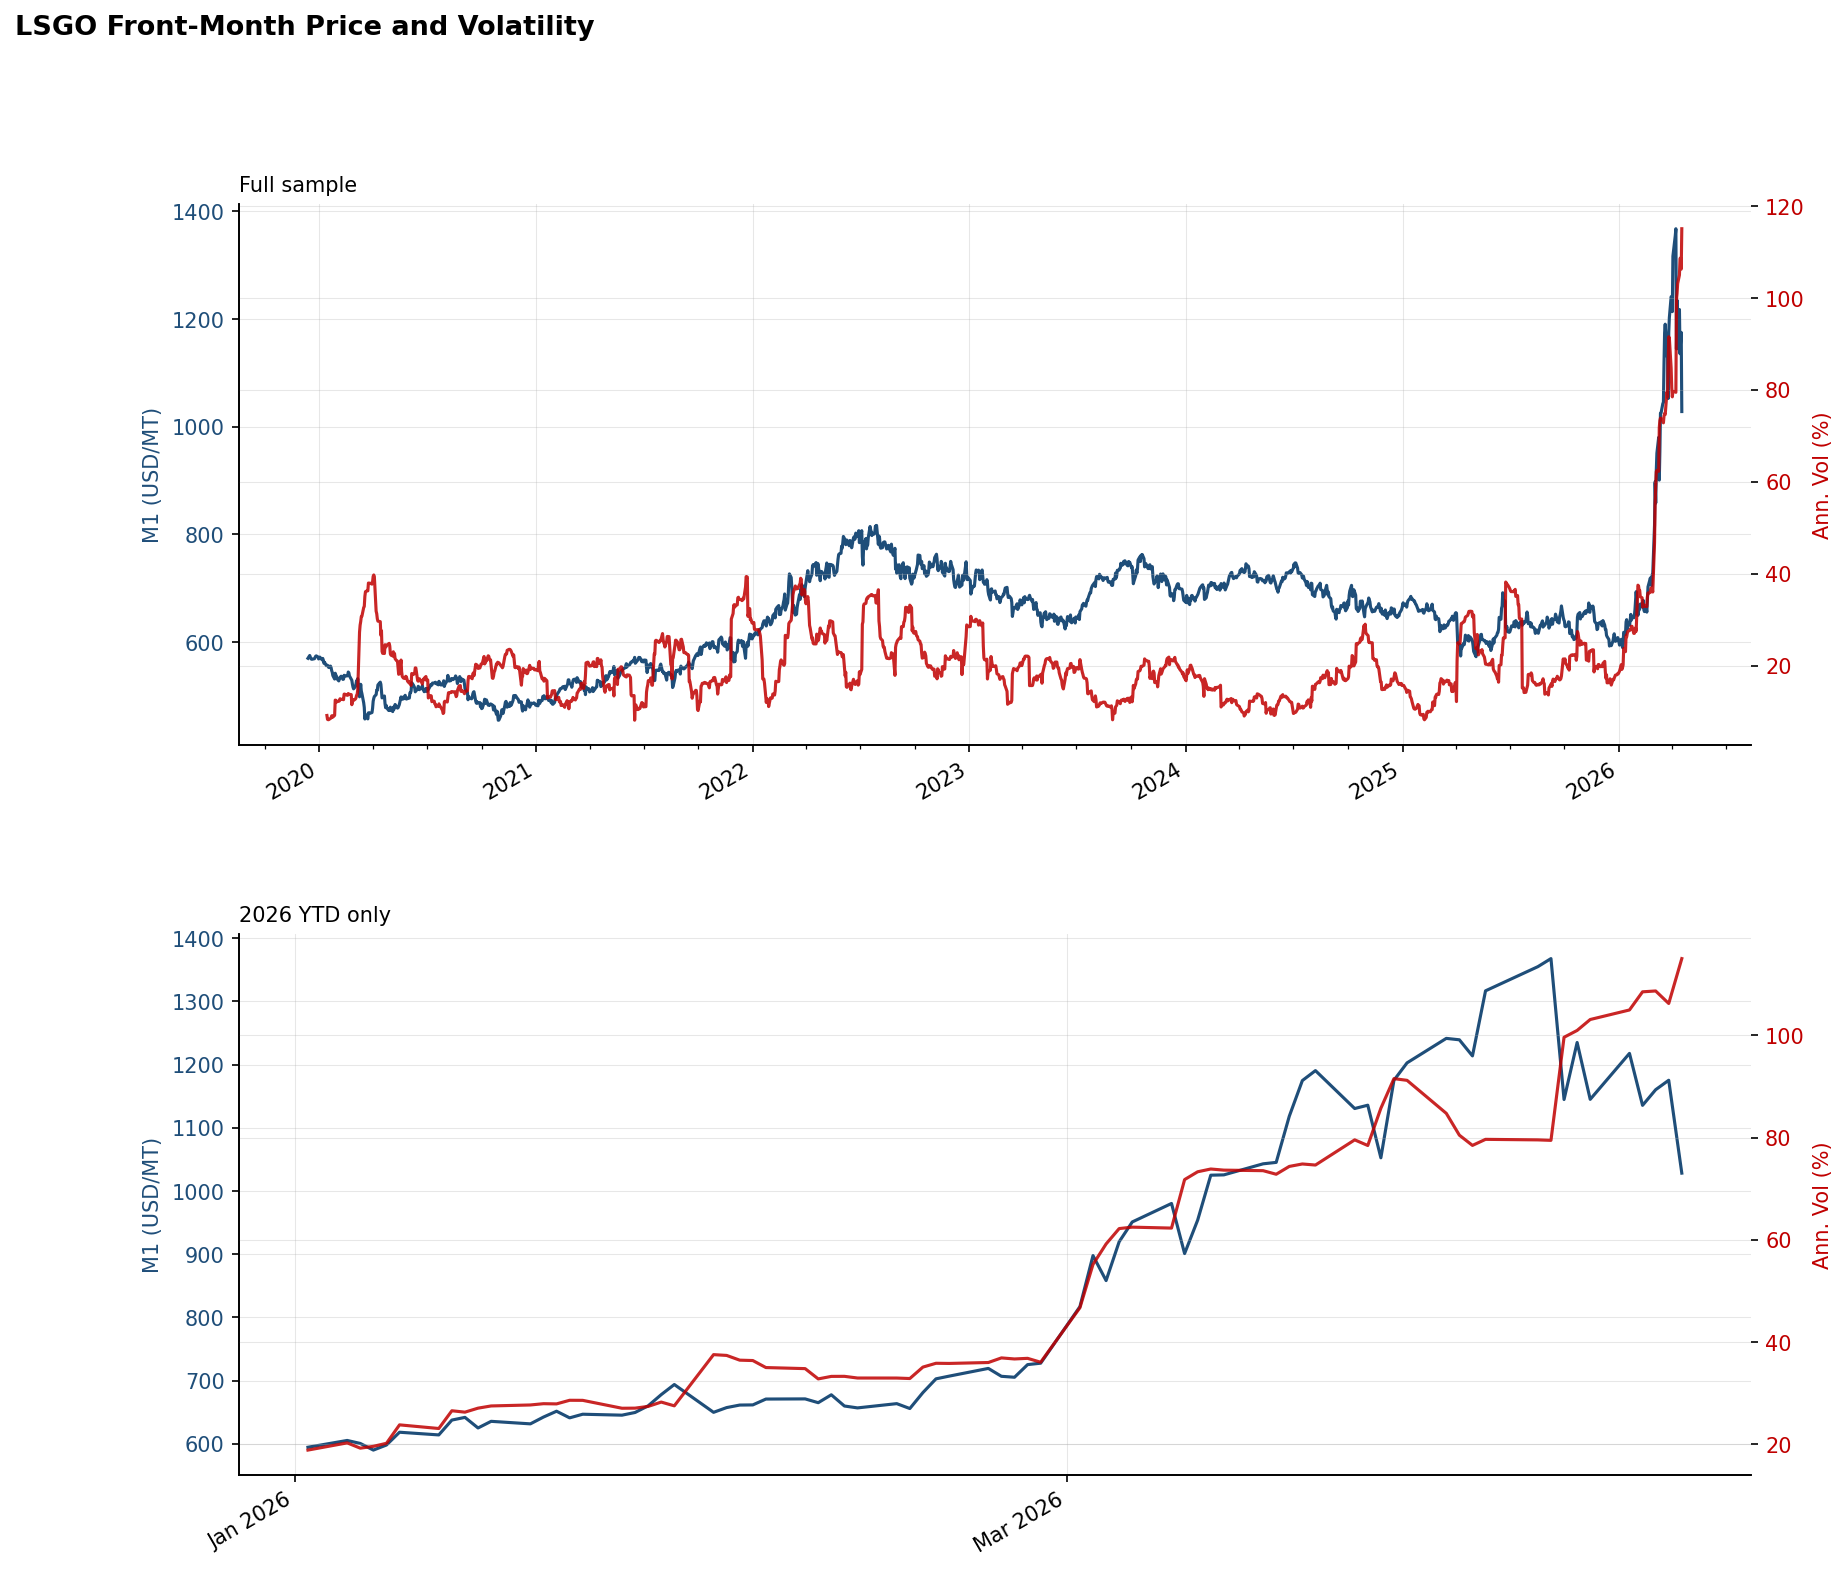
\includegraphics[width=\linewidth]{fig_03a_lsgo_price_vol.png}\\[0.2cm]
{\footnotesize\textit{\mbox{LSGO} price and 20-day annualised vol, full sample, event-overlay.}}
\end{center}

\vspace{0.3cm}

\begin{center}
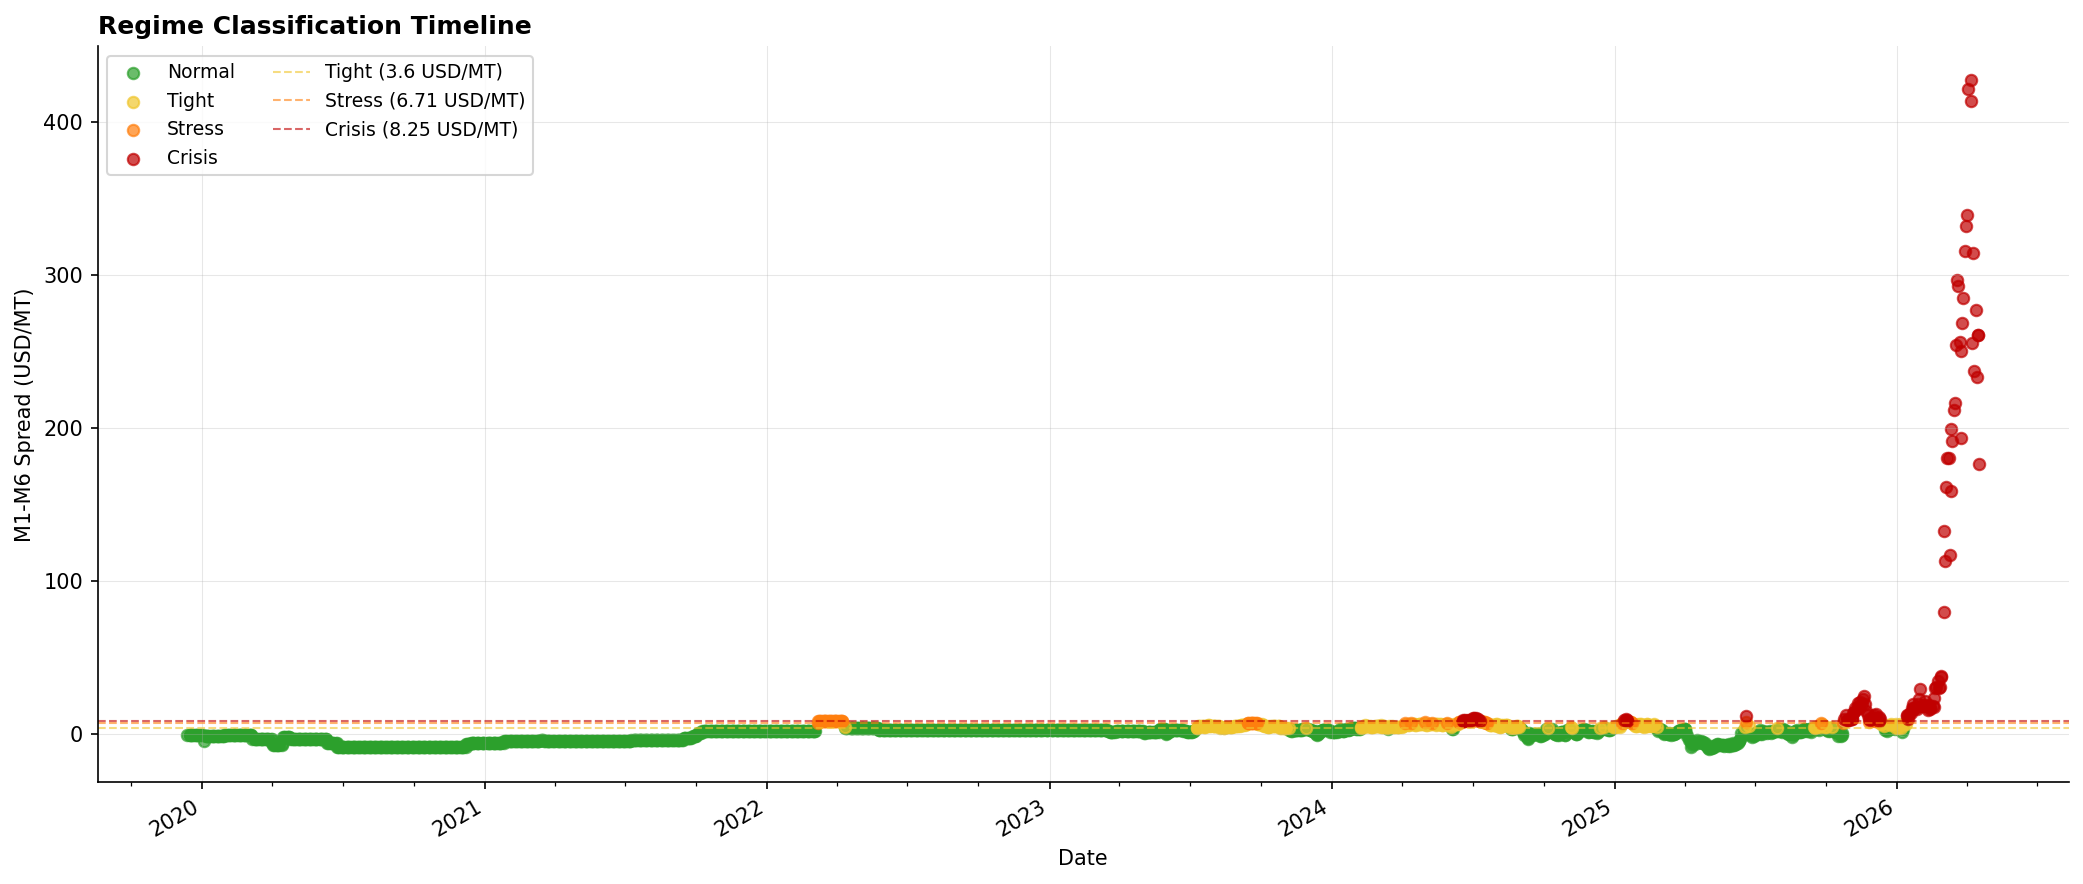
\includegraphics[width=\linewidth]{fig_03b_lsgo_regime.png}\\[0.2cm]
{\footnotesize\textit{CDF regime classification, IS-calibrated and OOS-evaluated.}}
\end{center}

\end{minipage}

\vspace{0.2cm}
\textbf{HMM cross-check (unsupervised regime detector).} A 2-state Gaussian HMM on the same M1-M6 spread series confirms the CDF regime break and \emph{flags Crisis $\sim$1 week before the CDF threshold breach}. BIC prefers K=2 over K=3 or 4 on this sample. The HMM is a sanity check, not an actionable early-warning trigger; full output and methodology are in the \S\ref{sec:15} appendix.

\vspace{0.2cm}

\newpage

% ============================================================================
% SECTION 4 — BRENT / WTI
% ============================================================================
\section{Brent and \mbox{WTI}: today against 36 years of context}\label{sec:4}

\textit{If \mbox{LSGO} tells the story of diesel specifically, Brent and \mbox{WTI} tell the story of the crude that feeds the refineries.}

\noindent\textcolor{obred}{\textbf{Desk decision.}} \emph{Brent prices geopolitical premium discontinuously --- paper-only risk models miss the jumps. The April Dated-vs-paper \$35/b dislocation is a basis-trade window, not textbook arbitrage.}

\vspace{0.2cm}

\noindent\begin{minipage}[t]{0.48\linewidth}\vspace{0pt}

Brent is backwardated 68.9\% of the full sample, similar to \mbox{LSGO}. The OOS distribution is bimodal: Normal on 82\% of days, Crisis on 17\%, Tight and Stress together fewer than 2\%. That shape tells you Brent prices geopolitical premium \emph{discontinuously}. One day it's normal, next day it's jumped to Crisis levels, and it skips the intermediate states. Paper-only risk models miss that jump because they assume smooth transitions.

The Dated-vs-paper dislocation in April is the cleanest physical-paper event in the sample. Dated printed \textbf{144.42 USD/bbl} on 7 April while the Jun-26 futures contract settled at 109.27, a 35-dollar cash-over-paper gap. The Dated file covers 69 days only (2 Jan to 14 Apr), so this is an event study, not a basis distribution. The setup, for a desk with physical Brent capability: long the physical cargo, short Brent paper, hold through the basis convergence. Not arbitrage in the textbook sense (cargo capacity, vetting, and credit gate execution); a basis-dislocation trade on the cleanest reference window of the cycle.

\mbox{WTI} is the tempered crude. Crisis regime frequency is around 13\% OOS, compared to 17\% for Brent and 31\% for \mbox{LSGO}. The mechanism is US-inland insulation: disrupted AG barrels price Brent first because they flow into the waterborne pool, and only show up in \mbox{WTI} once arb economics force US exports to Europe.

OPEC ASB Table 74 gives monthly Brent and \mbox{WTI} front-month settlements back to 1990. It's the long-history sanity check. Today's Brent level is top-quartile on a 36-year distribution but not unprecedented: 2008 hit \$134 peak, and 2011-2014 sustained above \$100.

\end{minipage}\hfill
\begin{minipage}[t]{0.48\linewidth}\vspace{0pt}

\begin{center}
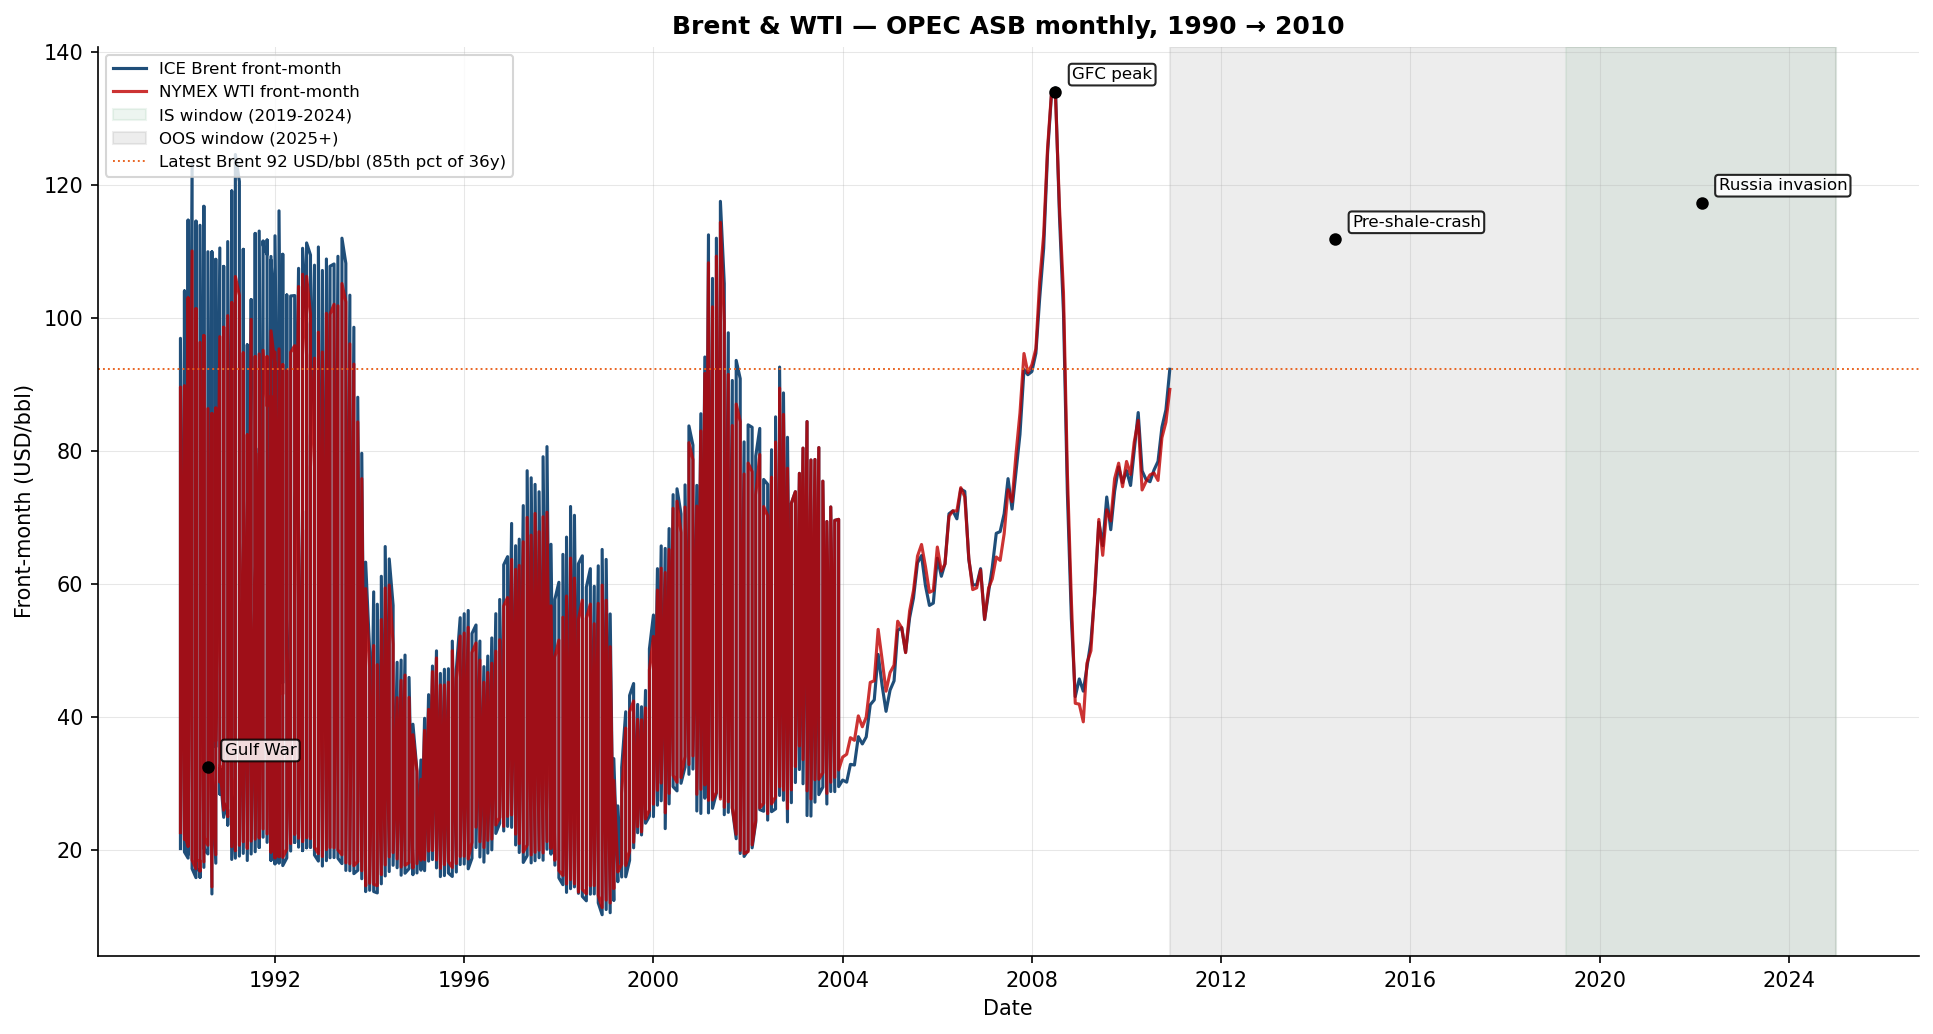
\includegraphics[width=\linewidth]{fig_04a_brent_longhistory.png}\\[0.2cm]
{\footnotesize\textit{Brent and \mbox{WTI} monthly front-month, 1990+, from OPEC ASB T74. IS/OOS shading matches the 2024-12-31 calibration cutoff.}}
\end{center}

\end{minipage}

\vspace{0.3cm}
\begin{center}
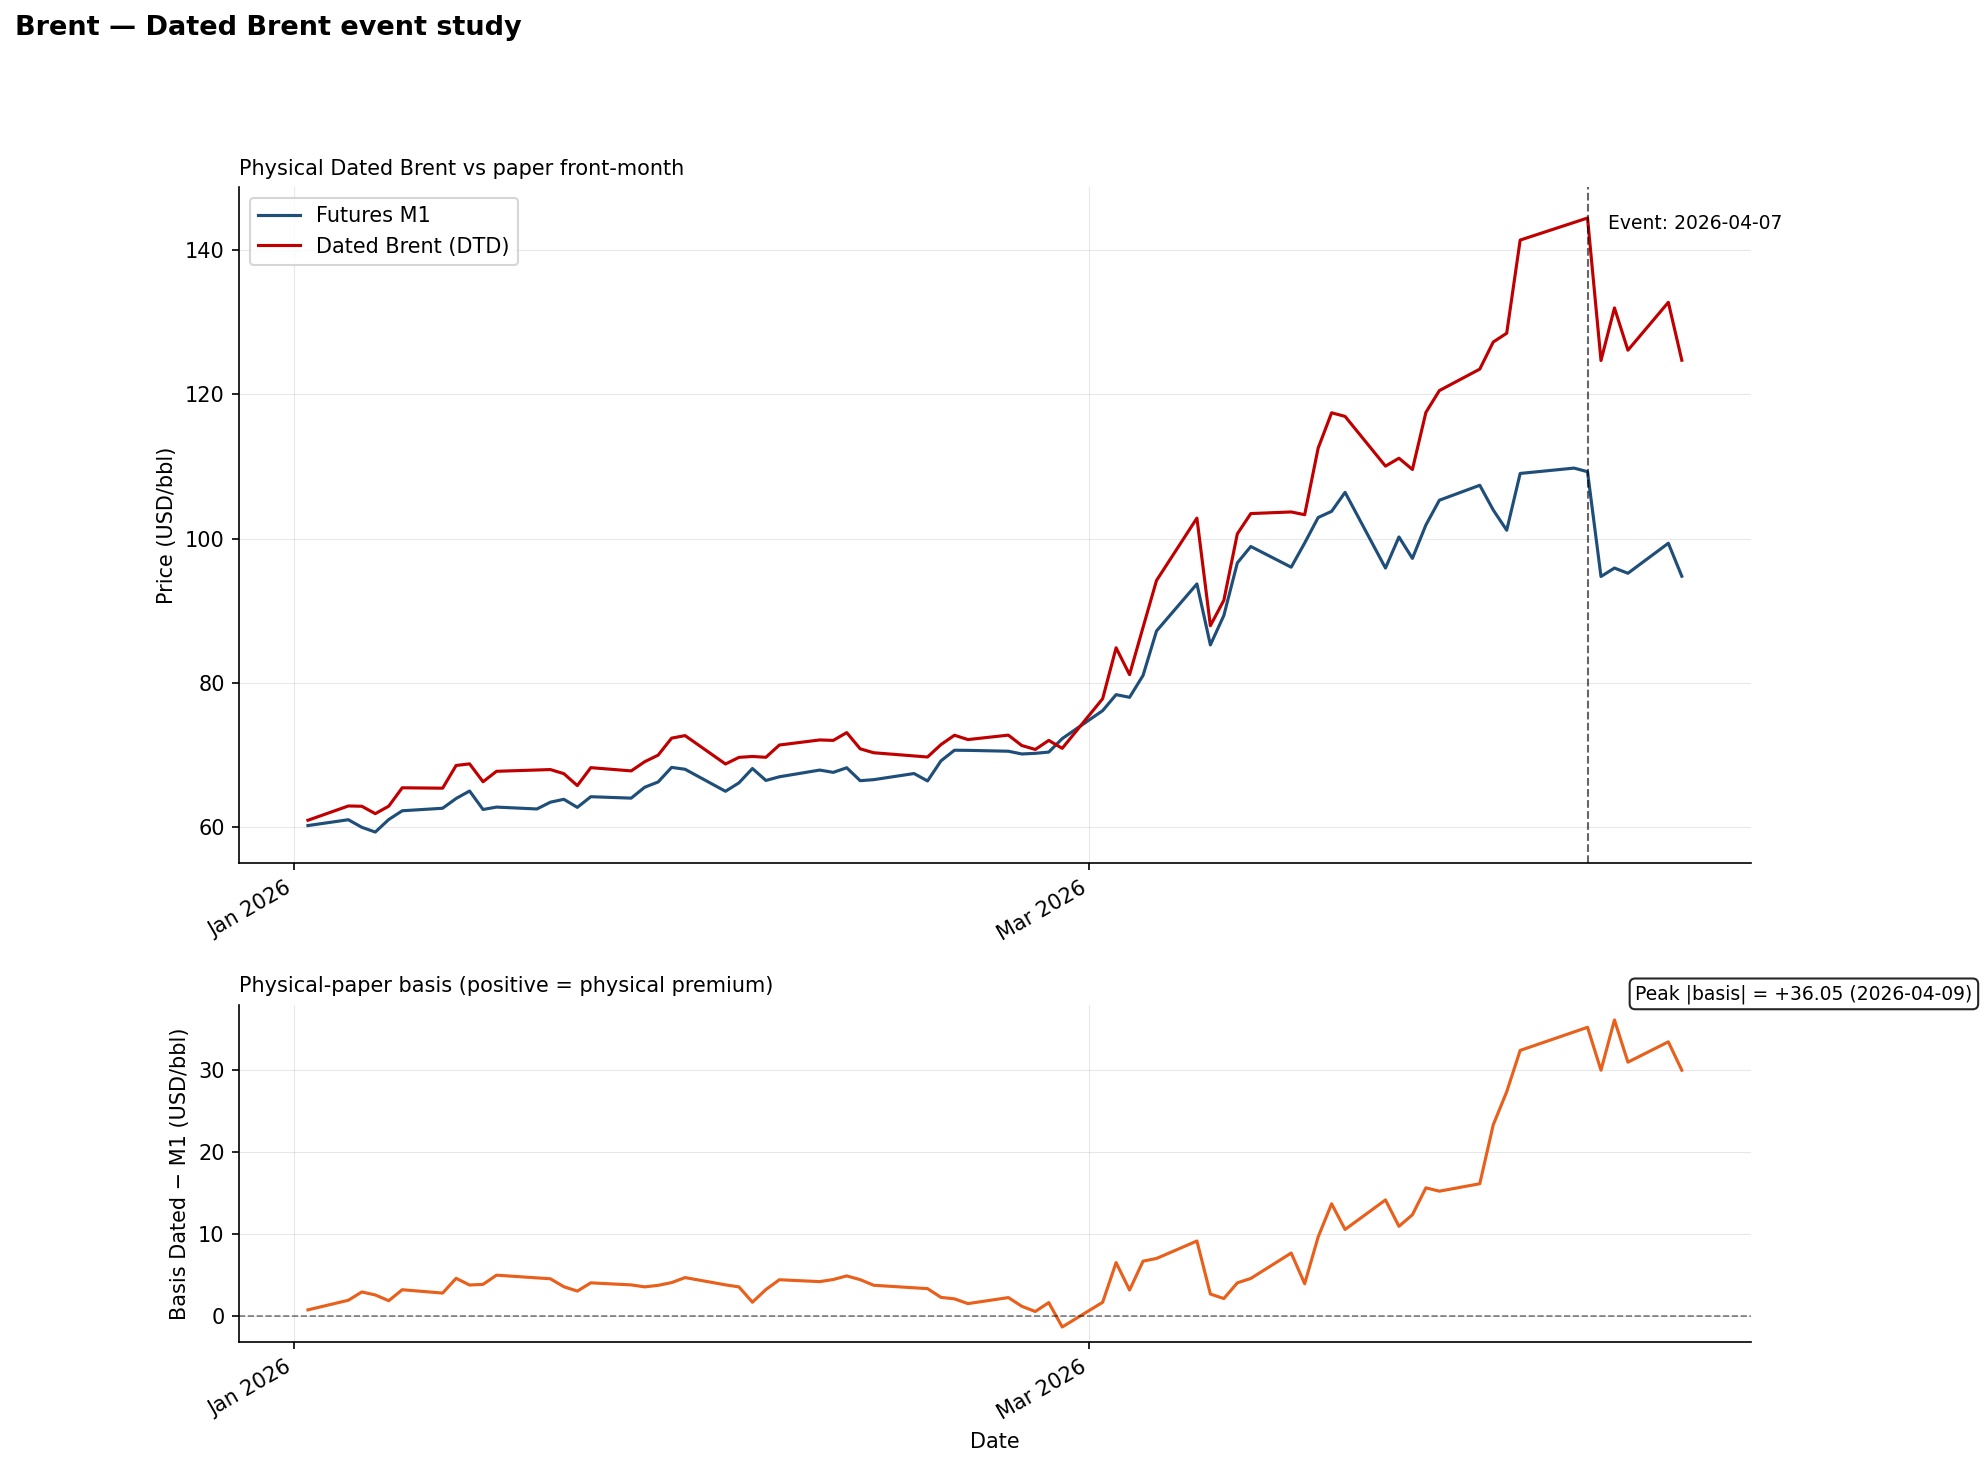
\includegraphics[width=0.62\linewidth]{fig_04b_dated_event_study.png}\\[0.1cm]
{\footnotesize\textit{Dated Brent against paper M1 during the April 2026 dislocation window.}}
\end{center}

\vspace{0.2cm}
%% [trailing bridge removed for pagination]

\newpage

% ============================================================================
% SECTION 5 — CROSS-MARKET
% ----------------------------------------------------------------------------
% Layout: page 7 = hero finding (full-width β callout + 2 charts side-by-side)
%         page 8 = supporting context (text + basin spread chart + methodology)
% ============================================================================
\needspace{20\baselineskip}
\section{Cross-market coupling: why static hedges break in a crisis}\label{sec:5}

\textit{The cleanest cross-project finding: the \mbox{NWE} crack hedge ratio is regime-dependent, not constant.}

\noindent\textcolor{obred}{\textbf{Desk decision.}} \emph{Hedge the live ULSD-Brent crack with $\beta = 0.92$ (production matched-M2$\times$M1, latest 30-day mean) $\rightarrow$ 46 short Brent lots per 50 kbbl crack-equivalent. Static $\beta = 0.4$ under-sizes by 50\%+.}

\vspace{0.15cm}

The \mbox{LSGO}-Brent $\Delta$M1-M3 correlation is 0.39 in \mbox{LSGO}'s Normal regime and 0.81 in Crisis --- a 2.1$\times$ ratio. A static hedge ratio calibrated on the pooled sample systematically under-sizes in Crisis windows. Annual coupling has trended up 2020--2026 (chart bottom-right), but the regime-conditional breakdown below shows the rise is driven by more time in Crisis, not a permanent re-coupling of the two curves. Normal regime: $\beta \approx -0.18$ (economically near-zero), confirming that in non-stressed markets ULSD cracks are not driven by crude but by refining margins and product balances.

\vspace{0.1cm}

\begin{callout}[Returns-based $\beta$ --- production-grade, regime-conditional]
\footnotesize
\textbf{Pipeline:} \texttt{cross\_market.py::matched\_rolling\_hedge\_ratio()}, calendar pairing wired via \texttt{futures\_calendar.py}; 60-day rolling-OLS on $\Delta$ log Crack vs $\Delta$ log Brent M1; conditioned per date on the LSGO M1-M6 regime flag. \emph{Output captured 2026-04-26 from} \texttt{outputs/reports/matched\_beta\_by\_regime.csv}.
\smallskip

\begin{center}
\begin{tabular}{@{}lrrrr@{}}
                                & \textbf{Normal} & \textbf{Crisis 2022} & \textbf{Crisis 2026} & \textbf{Latest 30d} \\
                                & \textbf{(full hist.)} & \textbf{invasion} & \textbf{Hormuz} & \textbf{(rolling)} \\
\midrule
Naïve M1$\times$M1 $\beta$       & $-$0.21         & $+$0.31              & $+$0.44              & $+$0.67 \\
Matched M2$\times$M1 $\beta$     & $-$0.18         & $+$0.31              & \textbf{$+$0.61}     & \textbf{$+$0.92} \\
Sample $n$                       & 1{,}147         & 26                   & 73                   & 30 \\
\end{tabular}
\end{center}
\smallskip

\textbf{Reading.} In \emph{Normal}, $\beta \approx 0$ — the matched ULSD-Brent crack floats nearly independent of Brent moves. In \emph{Crisis-2026 (active regime)}, matched $\beta = +0.61$ on average, but the relationship has accelerated: the latest 30-day window prints $+0.92$ and the Apr-17 single-day estimate is $+1.17$. The 2022 invasion was much milder ($\beta \approx +0.31$), so this is regime-of-its-kind — diesel-specific Hormuz pass-through, not a generic crisis pattern. \textbf{A static $\beta \approx 0.4$ pooled across regimes therefore under-sizes Brent risk on a Crisis-window crack position by roughly 50\% on the Crisis-2026 mean and by 2$\times$+ at the latest print.}

\textbf{Hedge translation (latest 30d, $\beta=0.92$).} For a 50,000-bbl long ULSD-crack-equivalent: \textbf{46 short Brent lots} (1 ICE Brent = 1,000 bbl). At regime-mean $\beta=0.61$: 31 lots. At static pooled $\beta=0.40$: 20 lots. Trade block sizes on the latest 30-day mean (live exposure); recalibrate weekly.

\textbf{Wiring complete.} The calendar pairing is in production (\S\ref{sec:14}); these numbers are computed end-to-end, not indicative. The 2022/2026 split is the single most desk-actionable finding in the deck --- each Crisis episode is unique, and the 2026 Hormuz dynamic is materially stronger than 2022.
\end{callout}

\vspace{0.15cm}

\noindent\begin{minipage}[t]{0.48\linewidth}\vspace{0pt}
\centerline{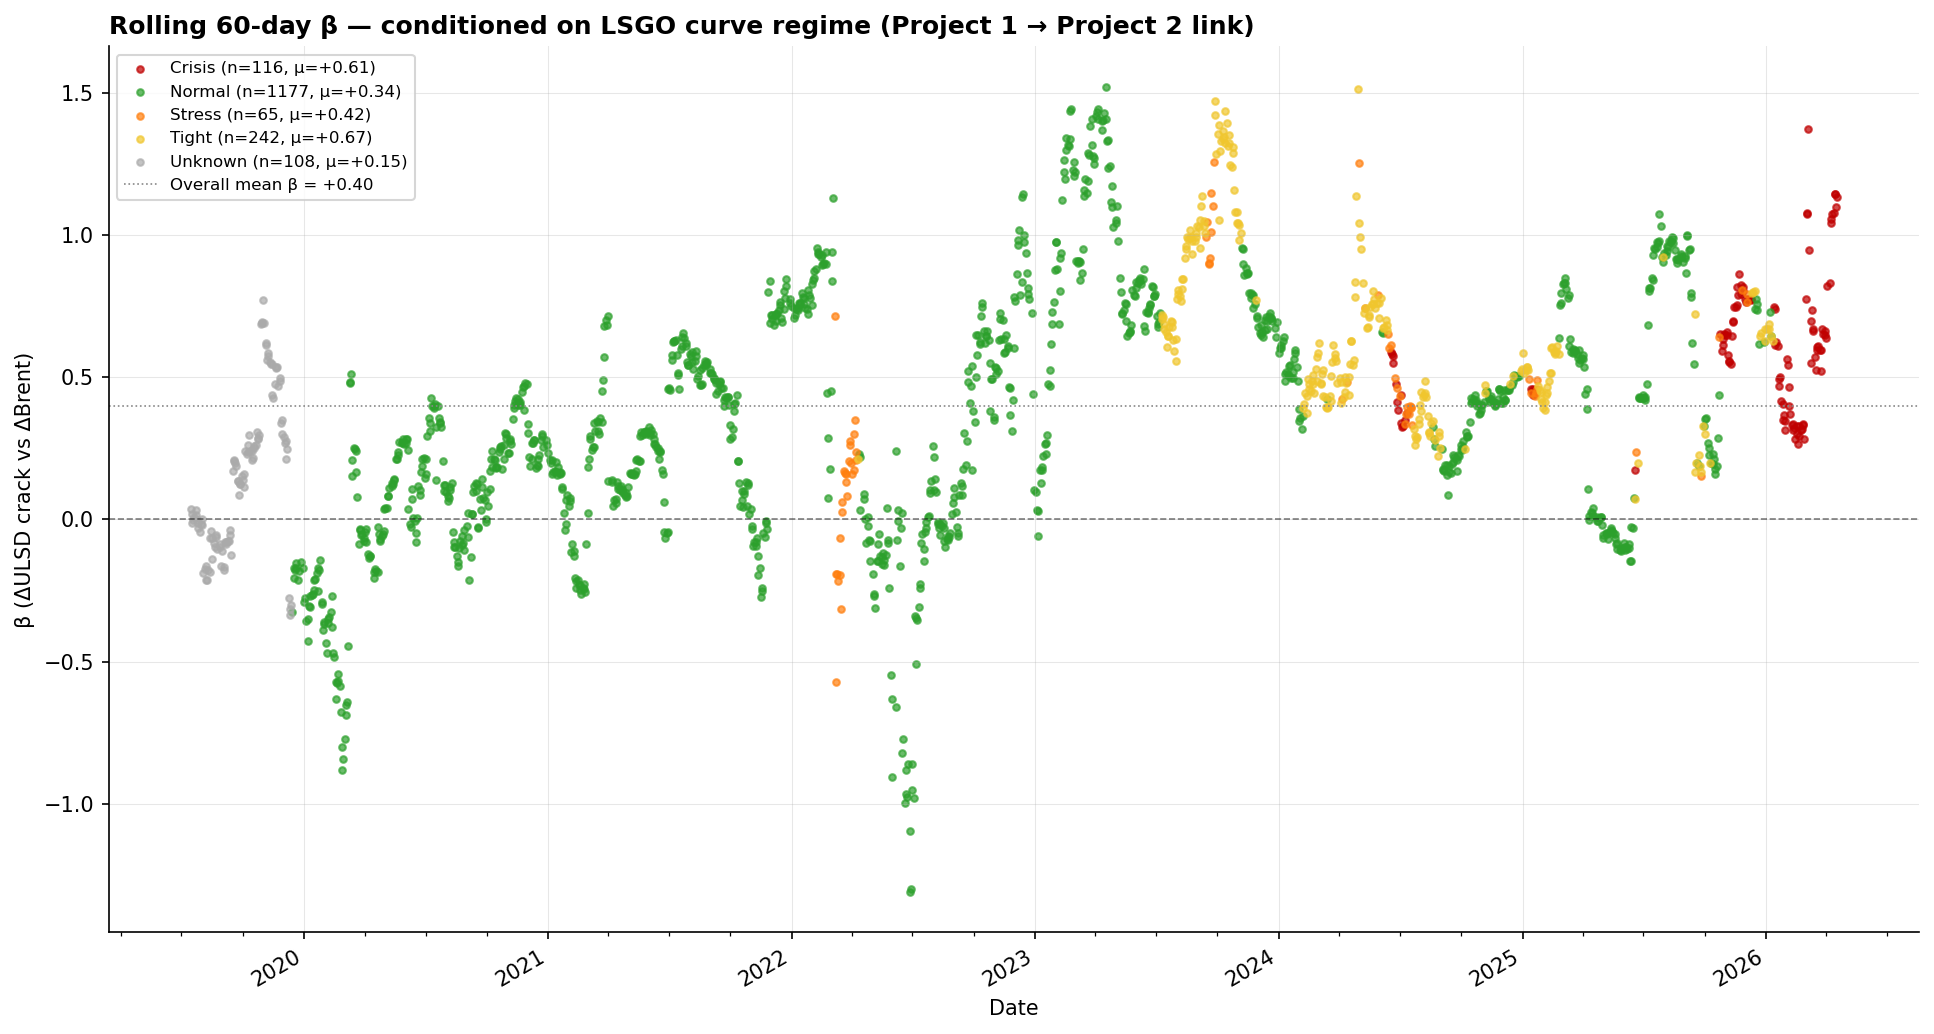
\includegraphics[width=\linewidth]{fig_05c_beta_by_regime.png}}
{\footnotesize\textit{Rolling-60d $\beta$ coloured by \mbox{LSGO} regime. Chart legend keeps v9 estimates; headline values in the callout above are production output.}}
\end{minipage}\hfill
\begin{minipage}[t]{0.48\linewidth}\vspace{0pt}
\centerline{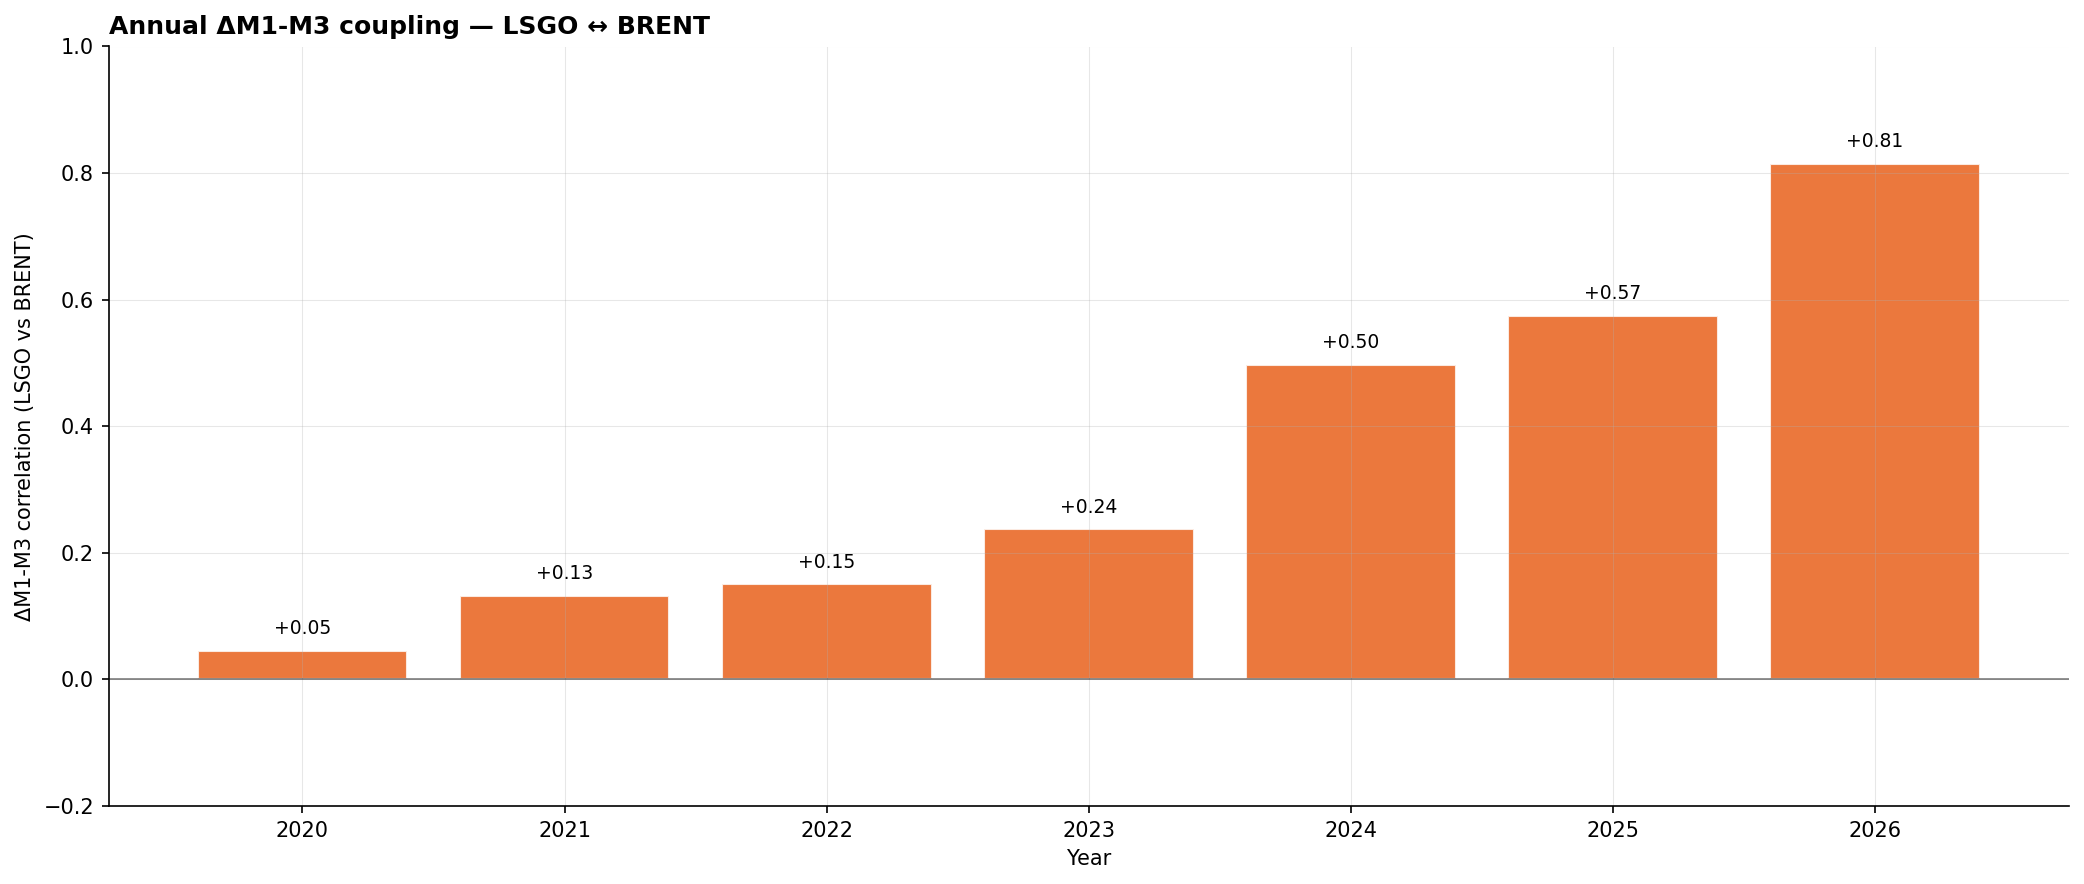
\includegraphics[width=\linewidth]{fig_05a_annual_coupling.png}}
{\footnotesize\textit{Annual \mbox{LSGO}-Brent $\Delta$M1-M3 correlation. Rising, but regime-driven.}}
\end{minipage}

\newpage

% ----------------------------------------------------------------------------
% PAGE 8 — supporting context: two specific moves + classifier methodology
% ----------------------------------------------------------------------------

\subsection*{Context: two specific moves in the rolling-$\beta$ series}

\noindent\begin{minipage}[t]{0.56\linewidth}\vspace{0pt}

\textbf{End-2020 correlation jump} ($\approx$0.3 $\rightarrow$ $\approx$0.6 inside a four-week window). OPEC+ rebalanced production on 3 December 2020, and the two commodities re-priced on shared macro signals from that point. I considered the vaccine-rollout story as a second contributor but the specific December timing matches OPEC+ more cleanly. \mbox{LSGO} and Brent had traded on different demand-side stories in early 2020 and converged when OPEC+ rebalanced supply.

\vspace{0.25cm}

\textbf{Brent--\mbox{WTI} basin widening (Hormuz pass-through).} Spread widened through March--April; \textbf{Apr 24 close $+$\$10.93/bbl} (Brent Jun \$105.33, \mbox{WTI} Jun \$94.40 --- both ICE settles), wider than the cycle peak quoted in earlier editions. Roughly 18 mb/d of pre-war AG loadings transit Hormuz and flow into the Brent-pricing waterborne pool. When those barrels were hit, Brent took the shock directly; \mbox{WTI} sat behind US export logistics and absorbs it only via arb-economics, hence the asymmetric move and the wider-than-cycle-peak basis on the day.

\end{minipage}\hfill
\begin{minipage}[t]{0.41\linewidth}\vspace{0pt}
\centerline{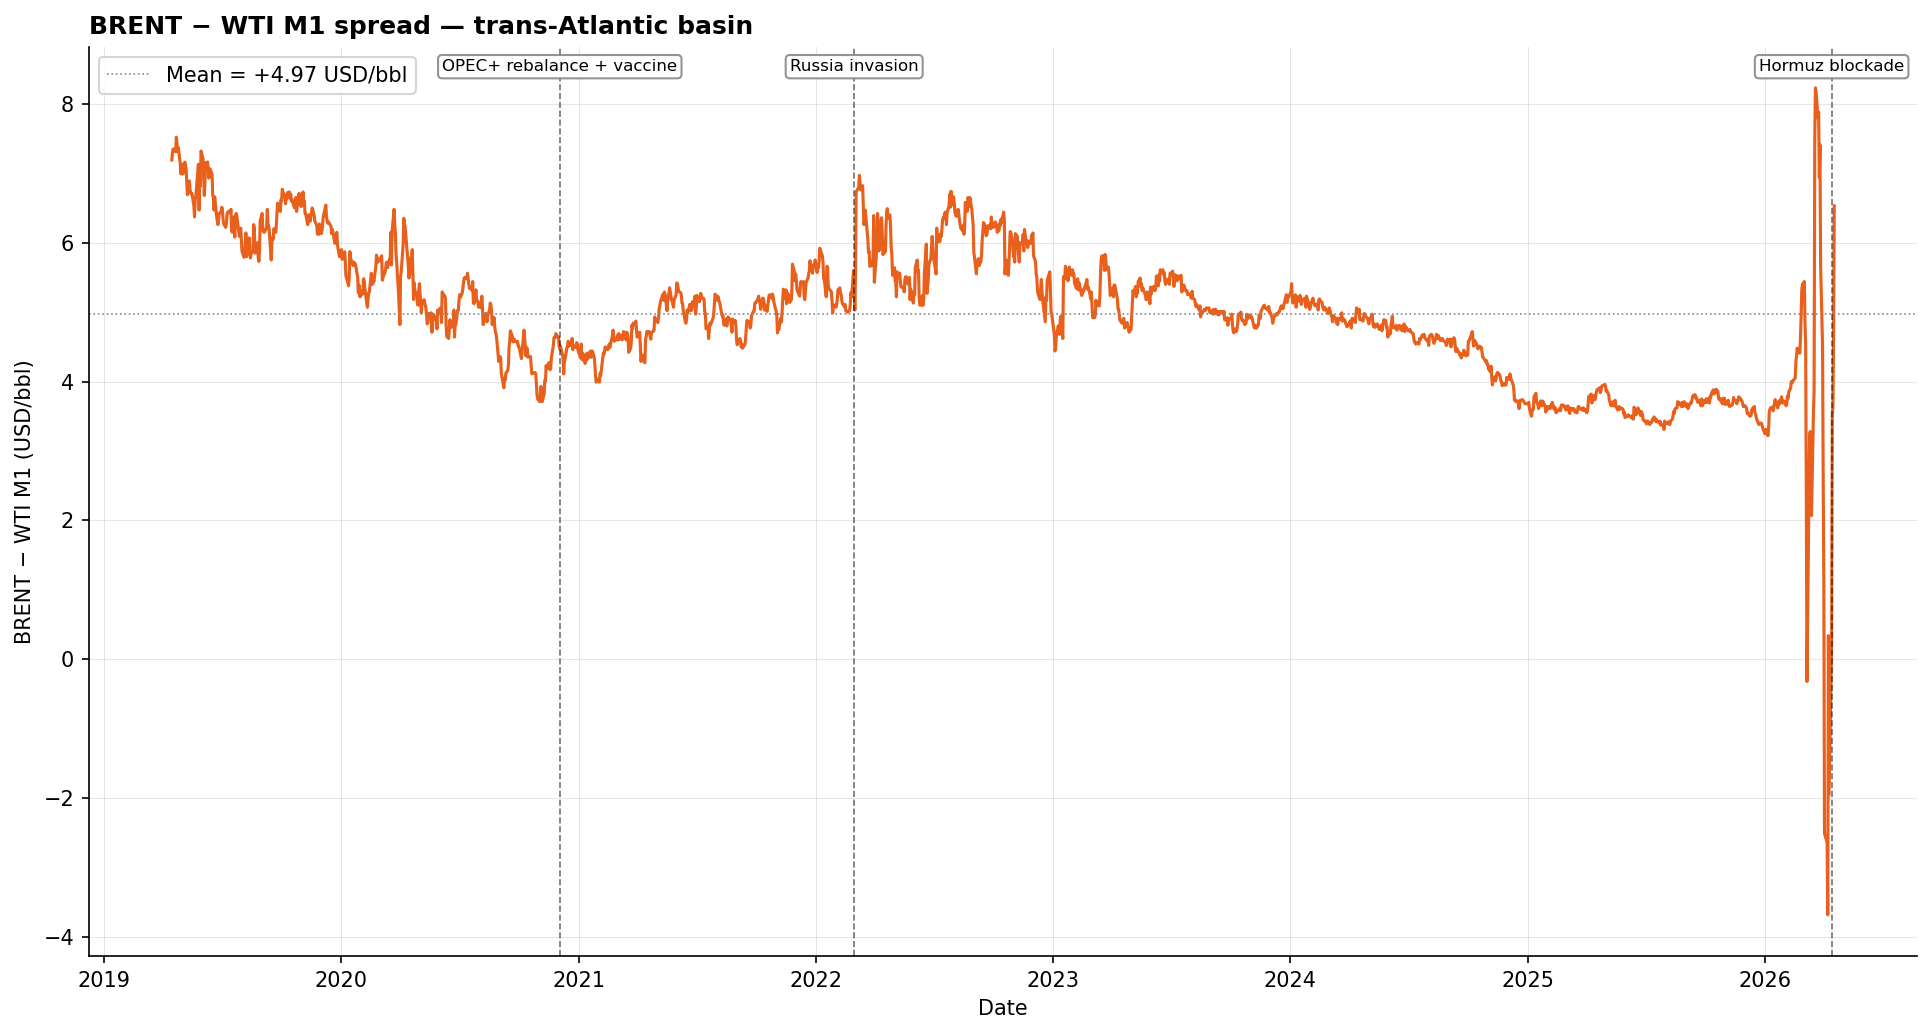
\includegraphics[width=\linewidth]{fig_05b_basin_spread.png}}
{\footnotesize\textit{Brent $-$ \mbox{WTI} M1 spread with event markers. Apr-24 close $+$\$10.93/bbl is the widest cycle print to date.}}
\end{minipage}

\vspace{0.4cm}

\begin{callout}[Methodology --- regime classifier and the 2-state collapse]
\footnotesize
Regime thresholds come from the pre-2025 CDF of \mbox{LSGO} M1-M6: Tight = 80th pct (3.60 USD/MT), Stress = 95th pct (6.71 USD/MT), Crisis = 99th pct (8.25 USD/MT). Same classifier used throughout the \texttt{ForwardCurveAnalysis} engine, reused without recalibration in the cross-regime $\beta$ statistic.

\smallskip
\textbf{Why two-state, not four:} the cross-regime $\beta$ here \emph{collapses} \{Tight, Stress, Crisis\} into a single \textit{Crisis} bucket and reports against \textit{Normal} only. Reason: Tight days ($n\approx48$ pre-2025) and Stress days ($n\approx12$) are too few to compute a stable per-bucket $\beta$ (var($\hat\beta$) blows up below $\sim$50 obs). Crisis days as 99th-pct are the rarest pre-2025 ($n\approx5$), so OOS Crisis ($n\approx120$) is what gives statistical power. Reporting four-bucket $\beta$ on this sample produces non-monotone noise; the 2-bucket Normal/Crisis split is the only one that supports a tradable hedge ratio.
\end{callout}

\newpage

% ============================================================================
% SECTION 6 — CRACKS
% ============================================================================
\section{\mbox{NWE} and Med cracks: the diesel signature}\label{sec:6}

\textit{Pick the right slate and the 2026 diesel-specific shock stops hiding inside the composite.}

\noindent\textcolor{obred}{\textbf{Desk decision.}} \emph{Trade ULSD-only crack, not 3-2-1 --- gasoline dilutes the diesel signal. The 2026 Crisis cluster only becomes visible once you remove gasoline from the slate.}

\vspace{0.2cm}

\noindent\begin{minipage}[t]{0.50\linewidth}\vspace{0pt}

\mbox{NWE} 3-2-1 peaked at 105.07 USD/bbl on 6 June 2022 in the post-invasion refining squeeze. The 2026 peak on the composite looks smaller, but that's a slate artefact: 3-2-1 weights gasoline twice as heavily as distillate, so a cross-product squeeze (2022, both legs widening) dwarfs a diesel-specific shock (2026, ULSD widens, EBOB stays tame).

Switching to the ULSD-only slate removes the dilution and makes the 2026 Crisis cluster visible in the regime chart. The default display hides the signal; you only see it once you pick the right slate for the shock you're actually looking at.

\textbf{External anchor.} OPEC ASB Table 76 publishes annual crack spreads back to 1983, including Rotterdam gasoil 10 ppm vs Brent. Directional agreement on the 4 overlap years; level offset ≈\$2/bbl consistent with 10 ppm Rotterdam barge vs under-10 ppm \mbox{NWE} CIF spec. Trend matches on sign and magnitude. Series are calendar-year means on both sides: the OPEC series is a calendar-year annual average, and the Platts-derived series is the annual mean of daily assessments, so the vertical offset is methodological (spec + regional assessment), not an alignment error.

\vspace{0.2cm}
\begin{callout}[Gross refining margin --- today]
\footnotesize
100 kbpd European refinery, current 3-2-1 crack at \textbf{$\sim$\$37/bbl} (Apr 24):
\smallskip

\textbf{Normal regime (90\% util)}: $\sim$\$1.22 B/year gross margin.
\smallskip

\textbf{Current regime (70\% util)}: $\sim$\$945 M/year gross margin.
\smallskip

Gross crack $\times$ throughput $\times$ utilisation, \emph{not} P\&L: no opex, no feedstock differential, no financing. Utilisation assumption 70\% blends IEA OMR April EU run-rate (\textit{as of 2026-04, $\approx$80\%}) with the partial Med derate flagged in the Apr-24 Platts European Marketscan refining commentary (Saras $\approx$ 65\%, Grandpuits $\approx$ 75\% on prior reporting). War-crisis logistics take roughly 22\% of nameplate off the table.
\end{callout}

\end{minipage}\hfill
\begin{minipage}[t]{0.48\linewidth}\vspace{0pt}

\begin{center}
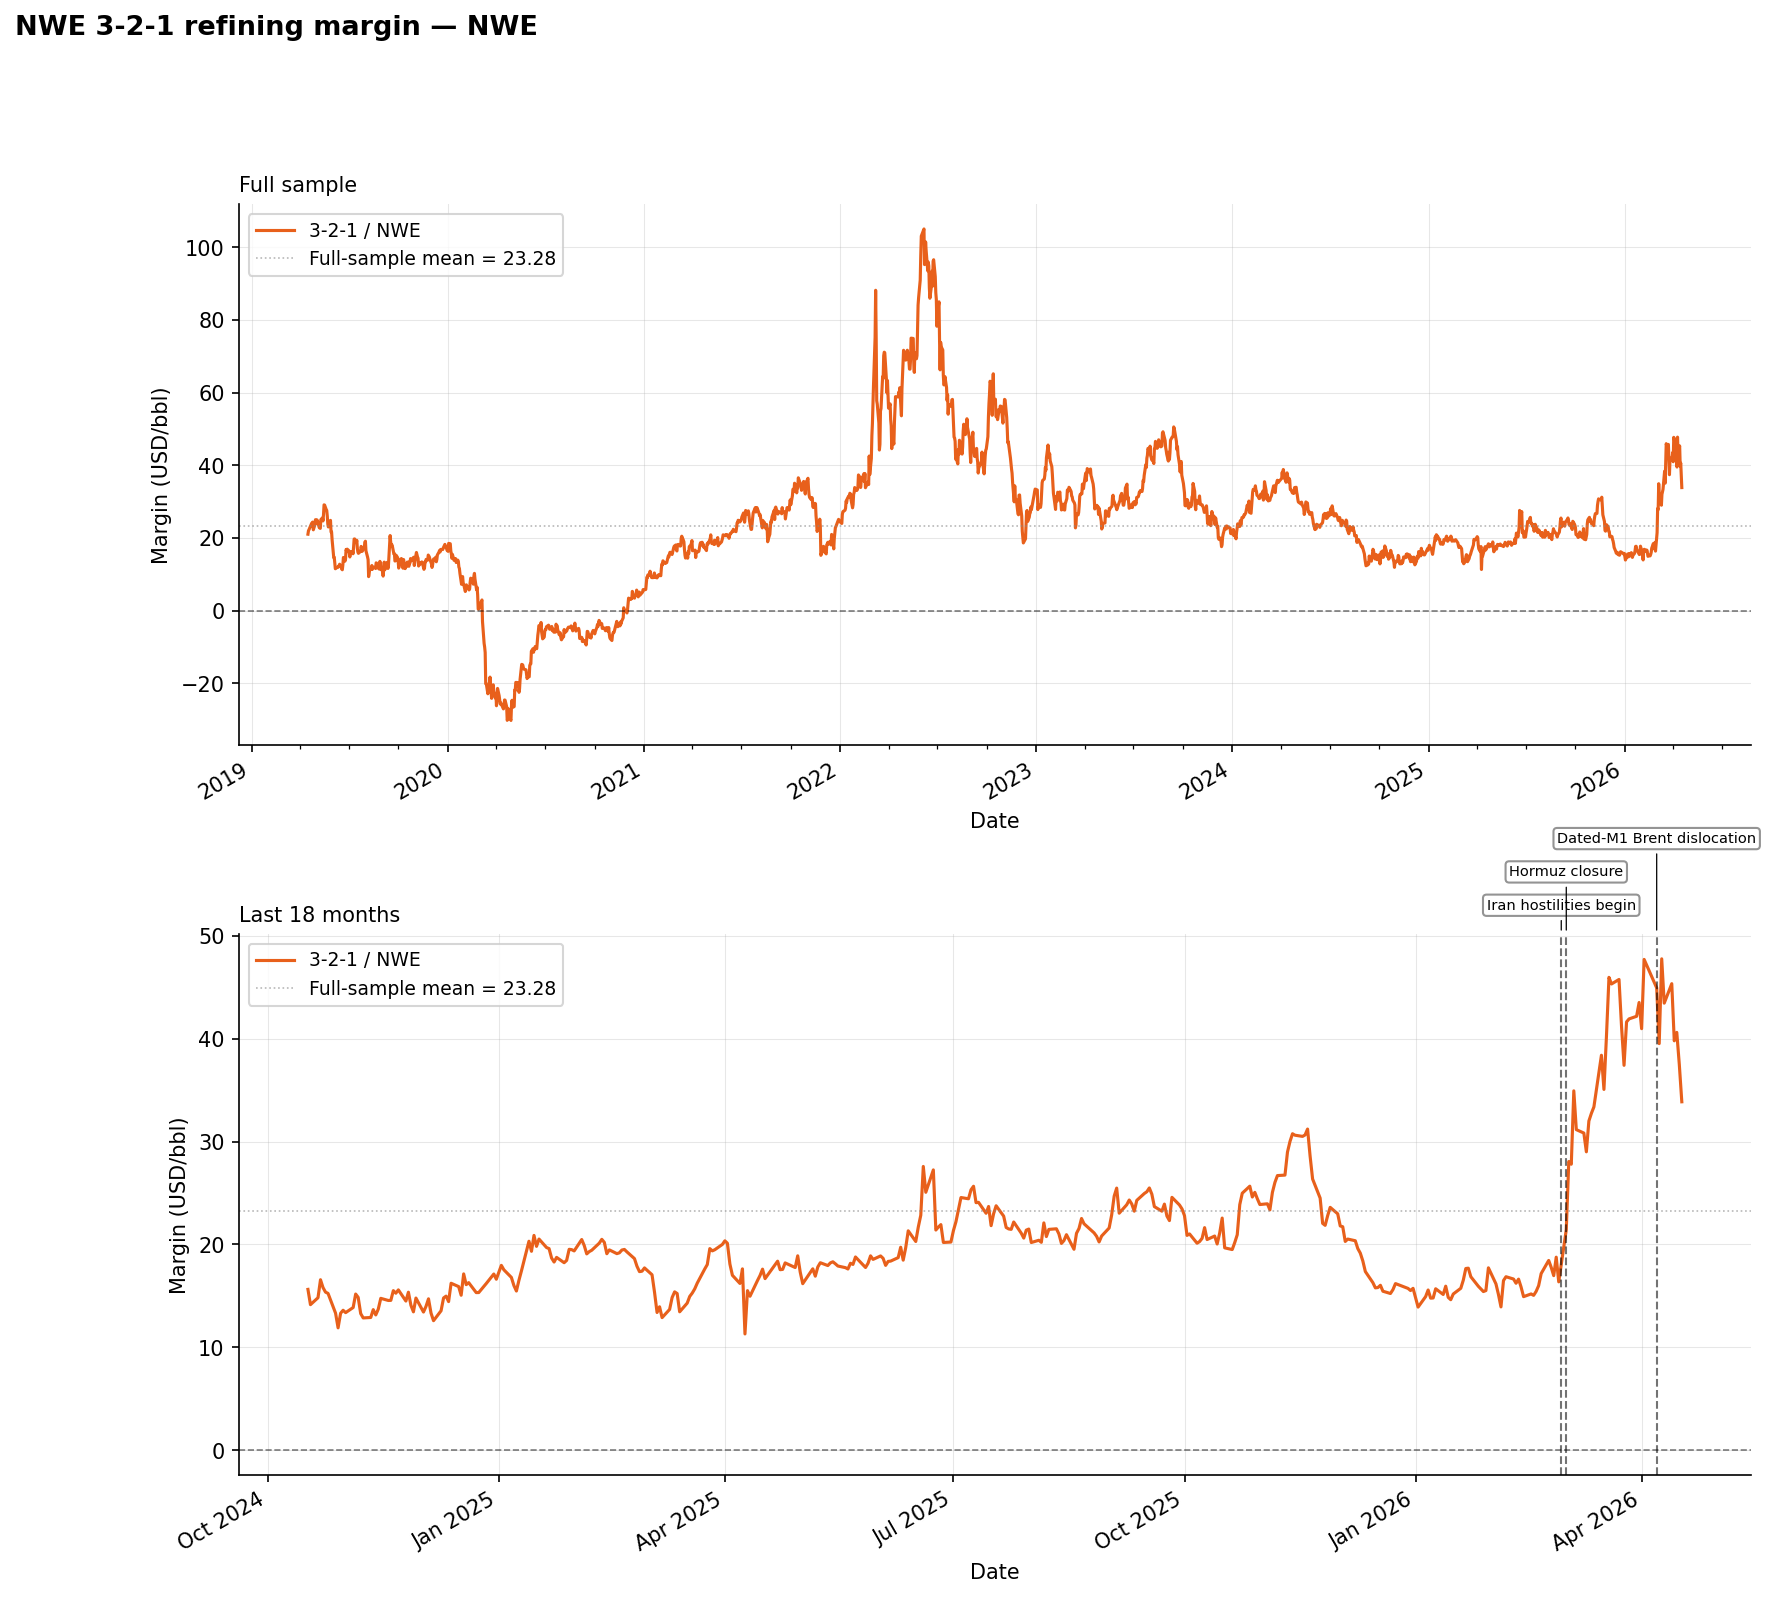
\includegraphics[width=\linewidth]{fig_06a_crack_timeseries.png}\\[0.2cm]
{\footnotesize\textit{3-2-1 \mbox{NWE} crack, full sample.}}
\end{center}

\vspace{0.2cm}

\begin{center}
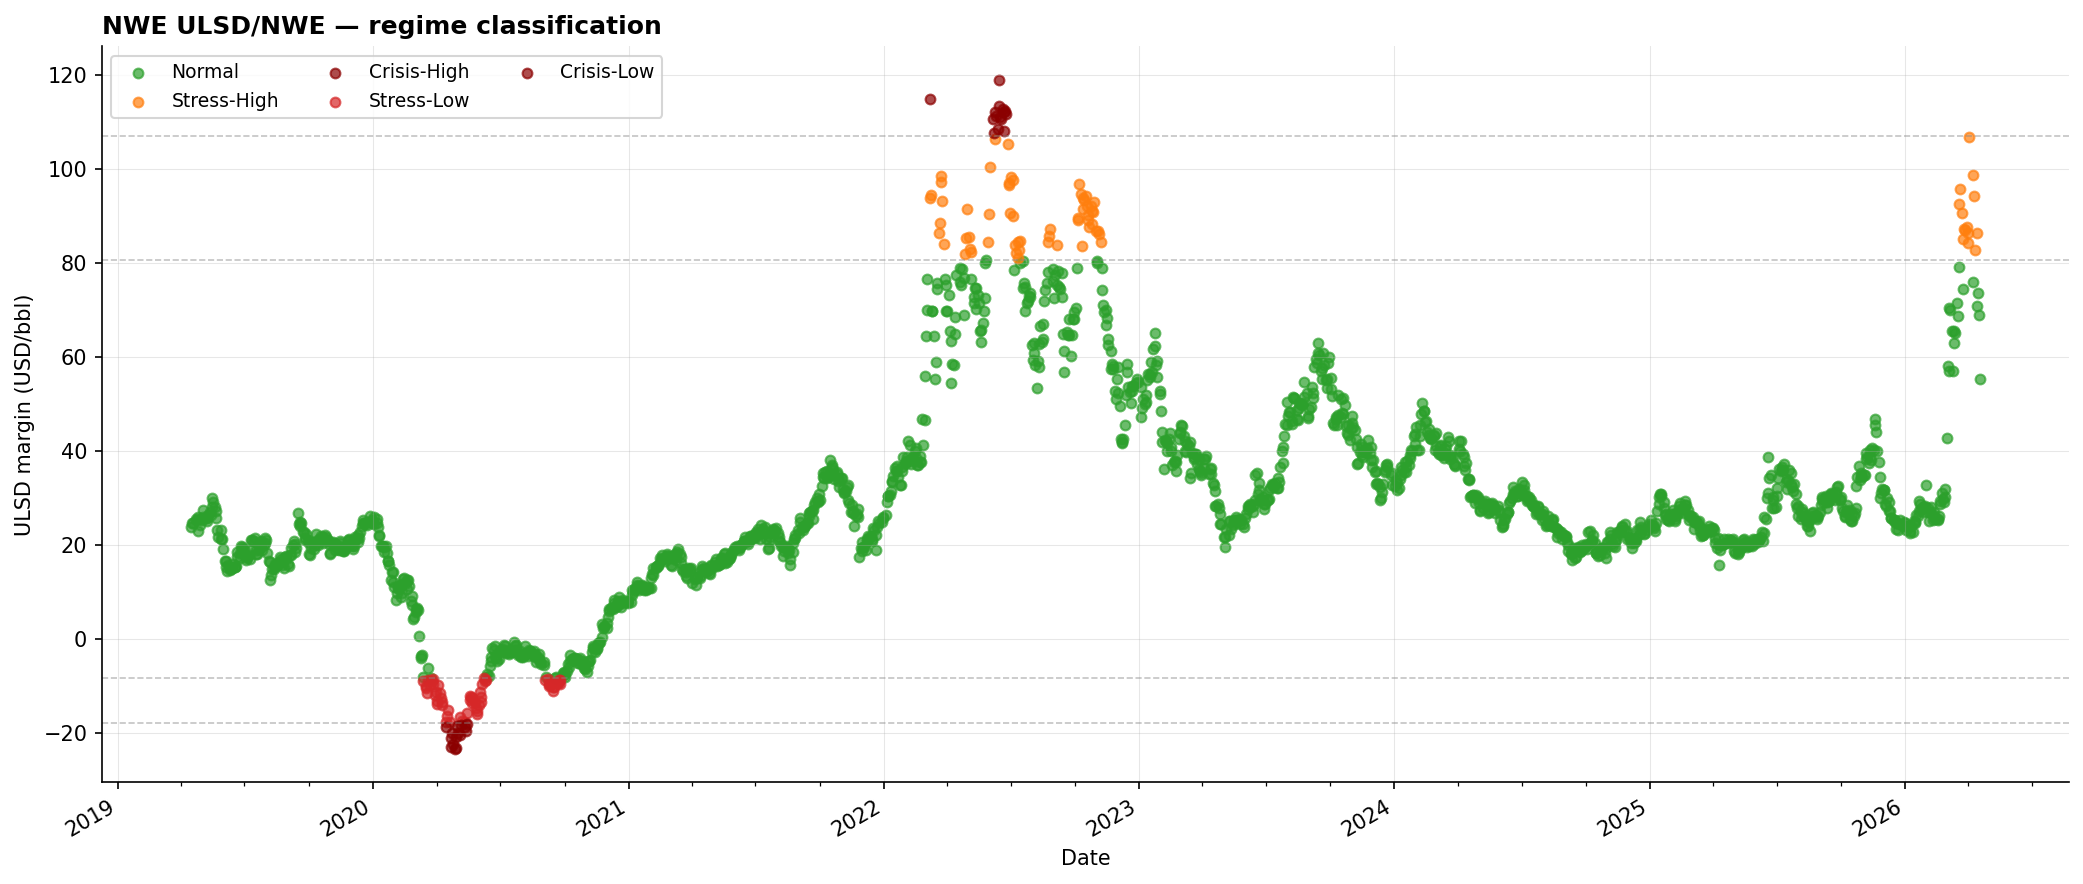
\includegraphics[width=\linewidth]{fig_06b_crack_regime.png}\\[0.2cm]
{\footnotesize\textit{ULSD slate, 2026 Crisis cluster visible once dilution is out of the way.}}
\end{center}

\end{minipage}

\vspace{0.2cm}
\begin{center}
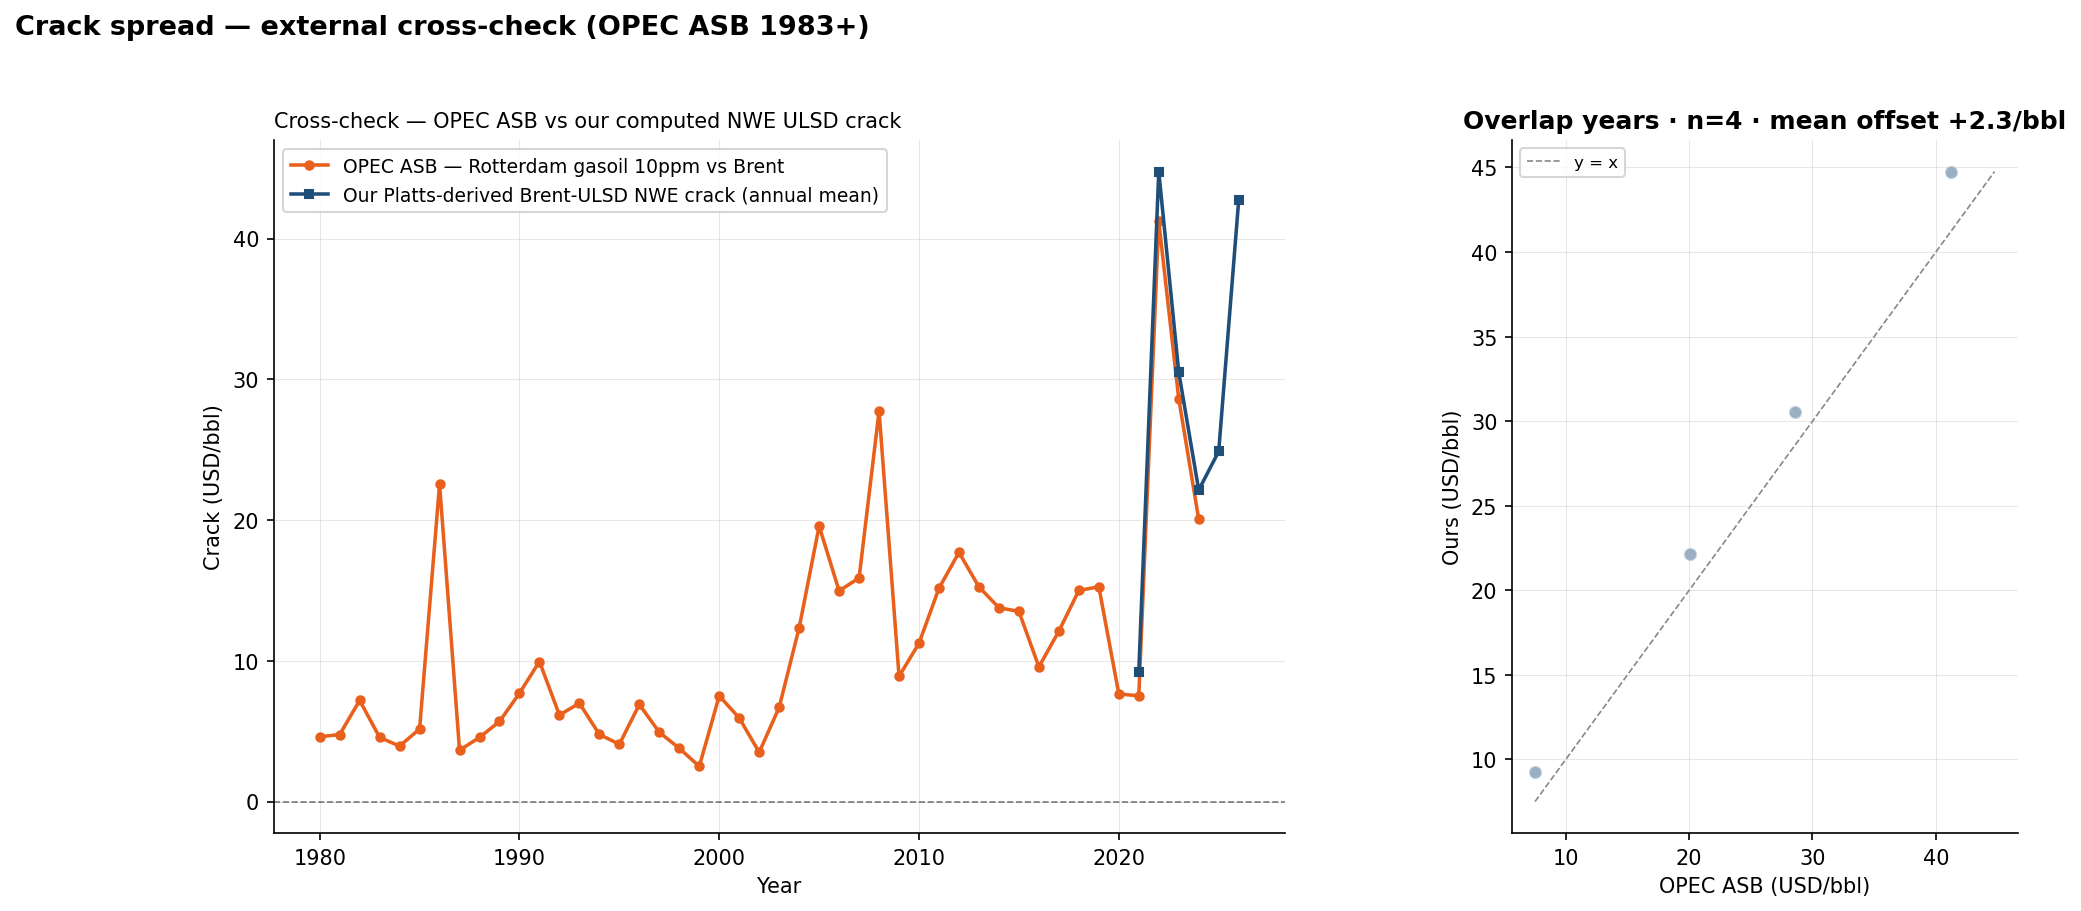
\includegraphics[width=0.78\linewidth]{fig_06c_opec_crosscheck.png}\\[0.1cm]
{\footnotesize\textit{Our \mbox{NWE} ULSD crack against OPEC ASB Rotterdam gasoil, calendar-year means on both sides; vertical offset is spec + assessment methodology.}}
\end{center}

\vspace{0.15cm}

\noindent\begin{minipage}[t]{0.55\linewidth}\vspace{0pt}
\textbf{Three Brent prices, not one.} The crack uses Brent M1 futures as the crude leg by default, but Brent has at least three distinct quoted prices: ICE M1 futures settlement, Platts spot (assessed close), and Dated Brent (16:30 London physical). They diverge by tens of dollars under stress; the April 2026 Dated-vs-M1 basis peaked around \$35/bbl, the largest physical-paper dislocation in the sample. Date windows are \emph{not aligned}: M1 from 2019, spot from 2021, Dated from 2-Jan-2026 only (69 trading days). Clean apples-to-apples basis is M1-vs-spot 2021$\rightarrow$, Dated-vs-M1 2026 only.
\end{minipage}\hfill%
\begin{minipage}[t]{0.42\linewidth}\vspace{0pt}
\begin{center}
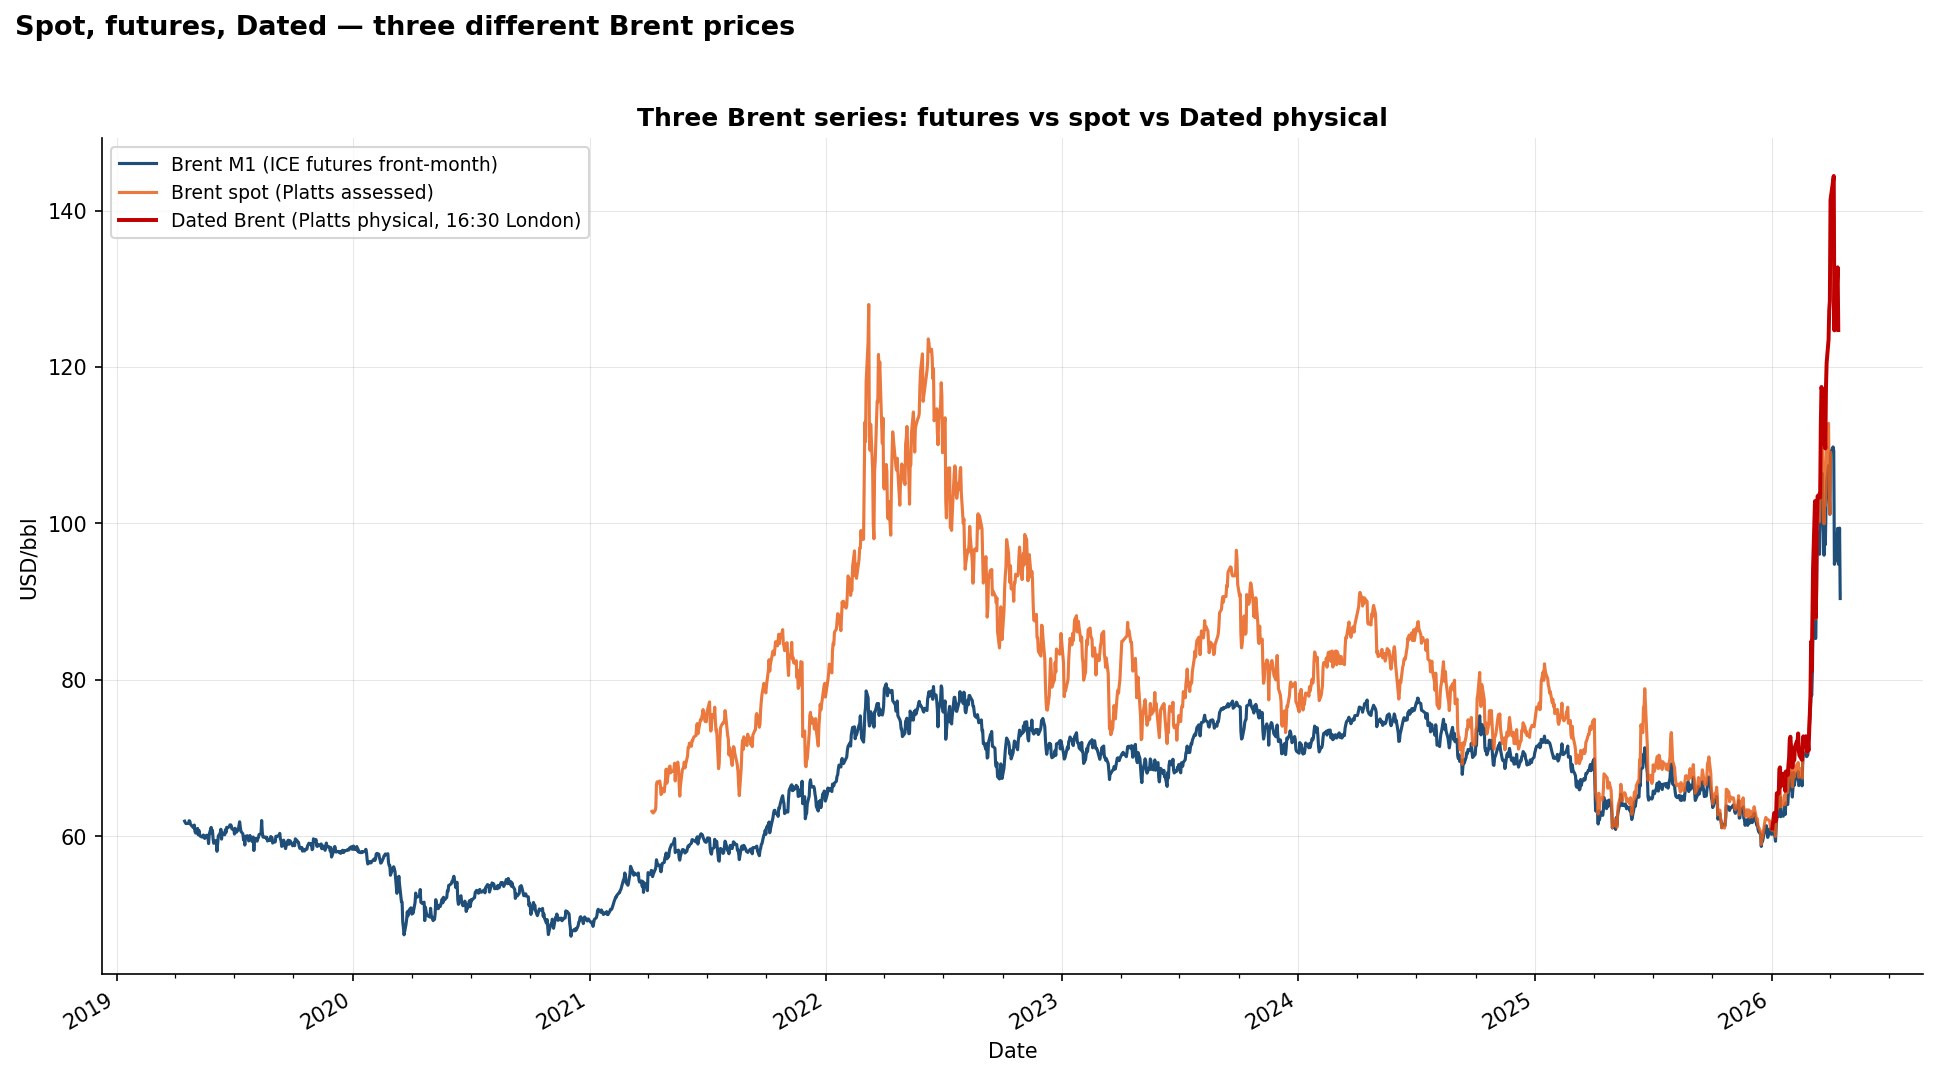
\includegraphics[width=\linewidth]{fig_06d_brent_three_tracks.png}\\[0.1cm]
{\footnotesize\textit{Brent M1 ICE futures (blue), Platts spot (orange), Dated Brent (red).}}
\end{center}
\end{minipage}

\vspace{0.1cm}

\newpage

% ============================================================================
% SECTION 7 — FUNDAMENTALS I
% ============================================================================
\section{Stocks and the 43-year picture of US refinery runs}\label{sec:7}

\textit{Today's utilisation looks extreme on a 5-year view, mid-range on a 43-year one.}

\noindent\textcolor{obred}{\textbf{Desk decision.}} \emph{US distillate stocks at the 50th percentile = no cushion against a supply shock --- the diesel leg responds harder than gasoline (84th pct, long). Refiner utilisation at 89.1\% is mid-range on the 1982+ series, not extreme.}

\vspace{0.2cm}

\noindent\begin{minipage}[t]{0.48\linewidth}\vspace{0pt}

US stocks right now aren't symmetric across products, and the asymmetry matters. As of the latest EIA Weekly Petroleum Status Report (week ending 2026-04-17), gasoline sits at the 84th percentile of its 2021-2026 weekly range (long), distillate at the 50th (no cushion), crude incl.\ SPR at the 72nd. Percentiles computed on PADD-aggregated stocks against a rolling 5-year weekly window. Structurally that means the diesel leg responds harder to a supply shock than the gasoline leg, which is what the 2026 OOS data has shown.

The long-history US refinery utilisation chart is probably the most contrarian single finding in this section. The latest EIA print is \textbf{89.1\%} (week to 17-Apr-2026), still top third on a 5-year view but only the 44th percentile of the full 1982+ weekly series. That reframes the "refineries are tight" narrative as tight vs recent memory, not vs 43-year history.

SPR stays on the chart as a reminder. Hormuz dominates the 2026 tape, but a 45\% peak-to-trough drawdown (291 Mbbl net release) has to reverse eventually, and the refill itself is a multi-year sour-crude demand story the market hasn't begun to price.

\end{minipage}\hfill
\begin{minipage}[t]{0.48\linewidth}\vspace{0pt}

\begin{center}
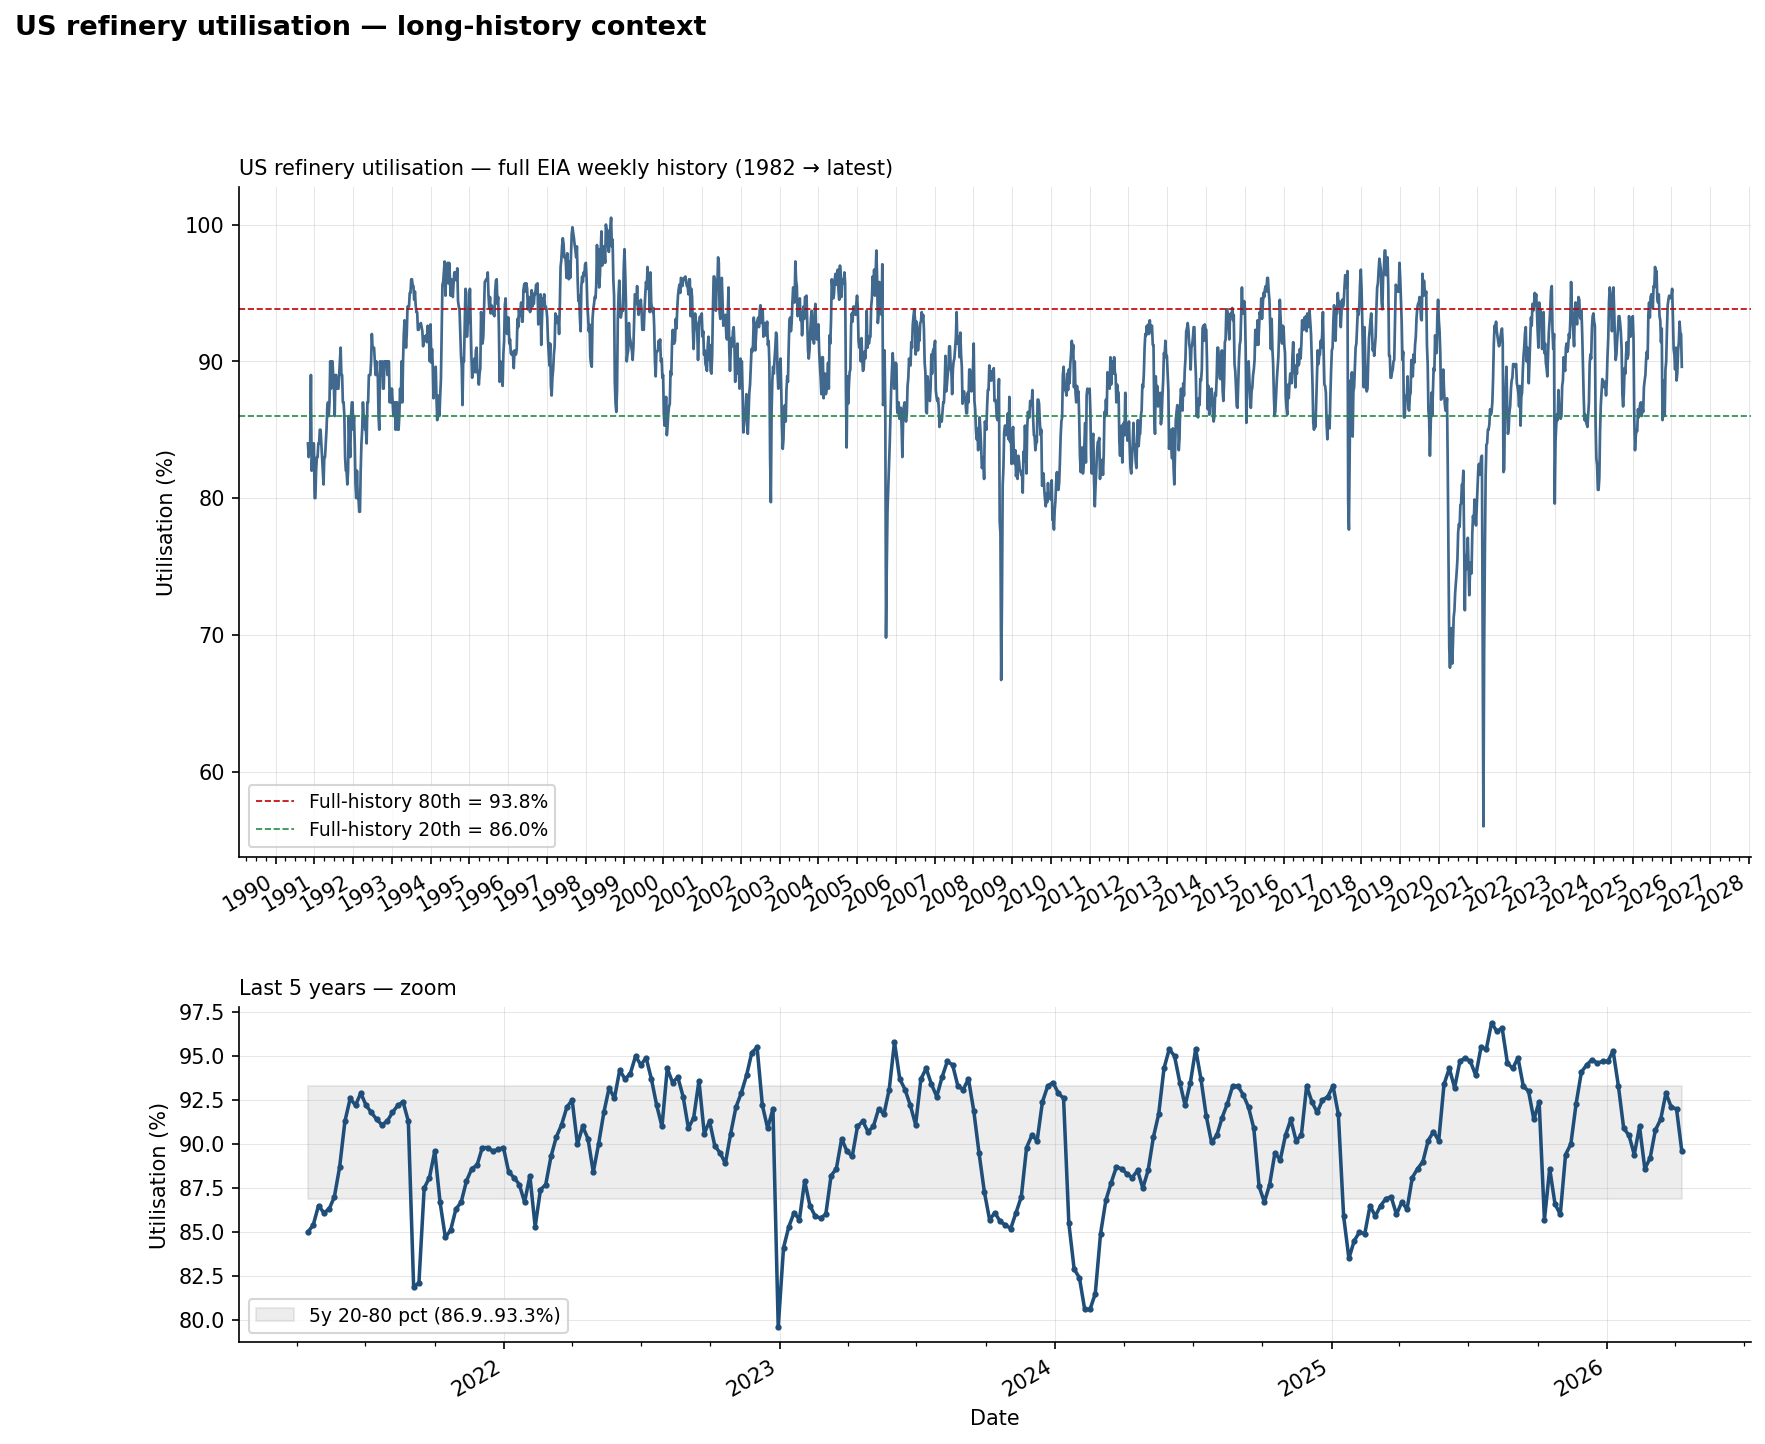
\includegraphics[width=\linewidth]{fig_07a_us_util_long.png}\\[0.2cm]
{\footnotesize\textit{US refinery utilisation, full EIA 1982+ weekly.}}
\end{center}

\vspace{0.2cm}

\begin{center}
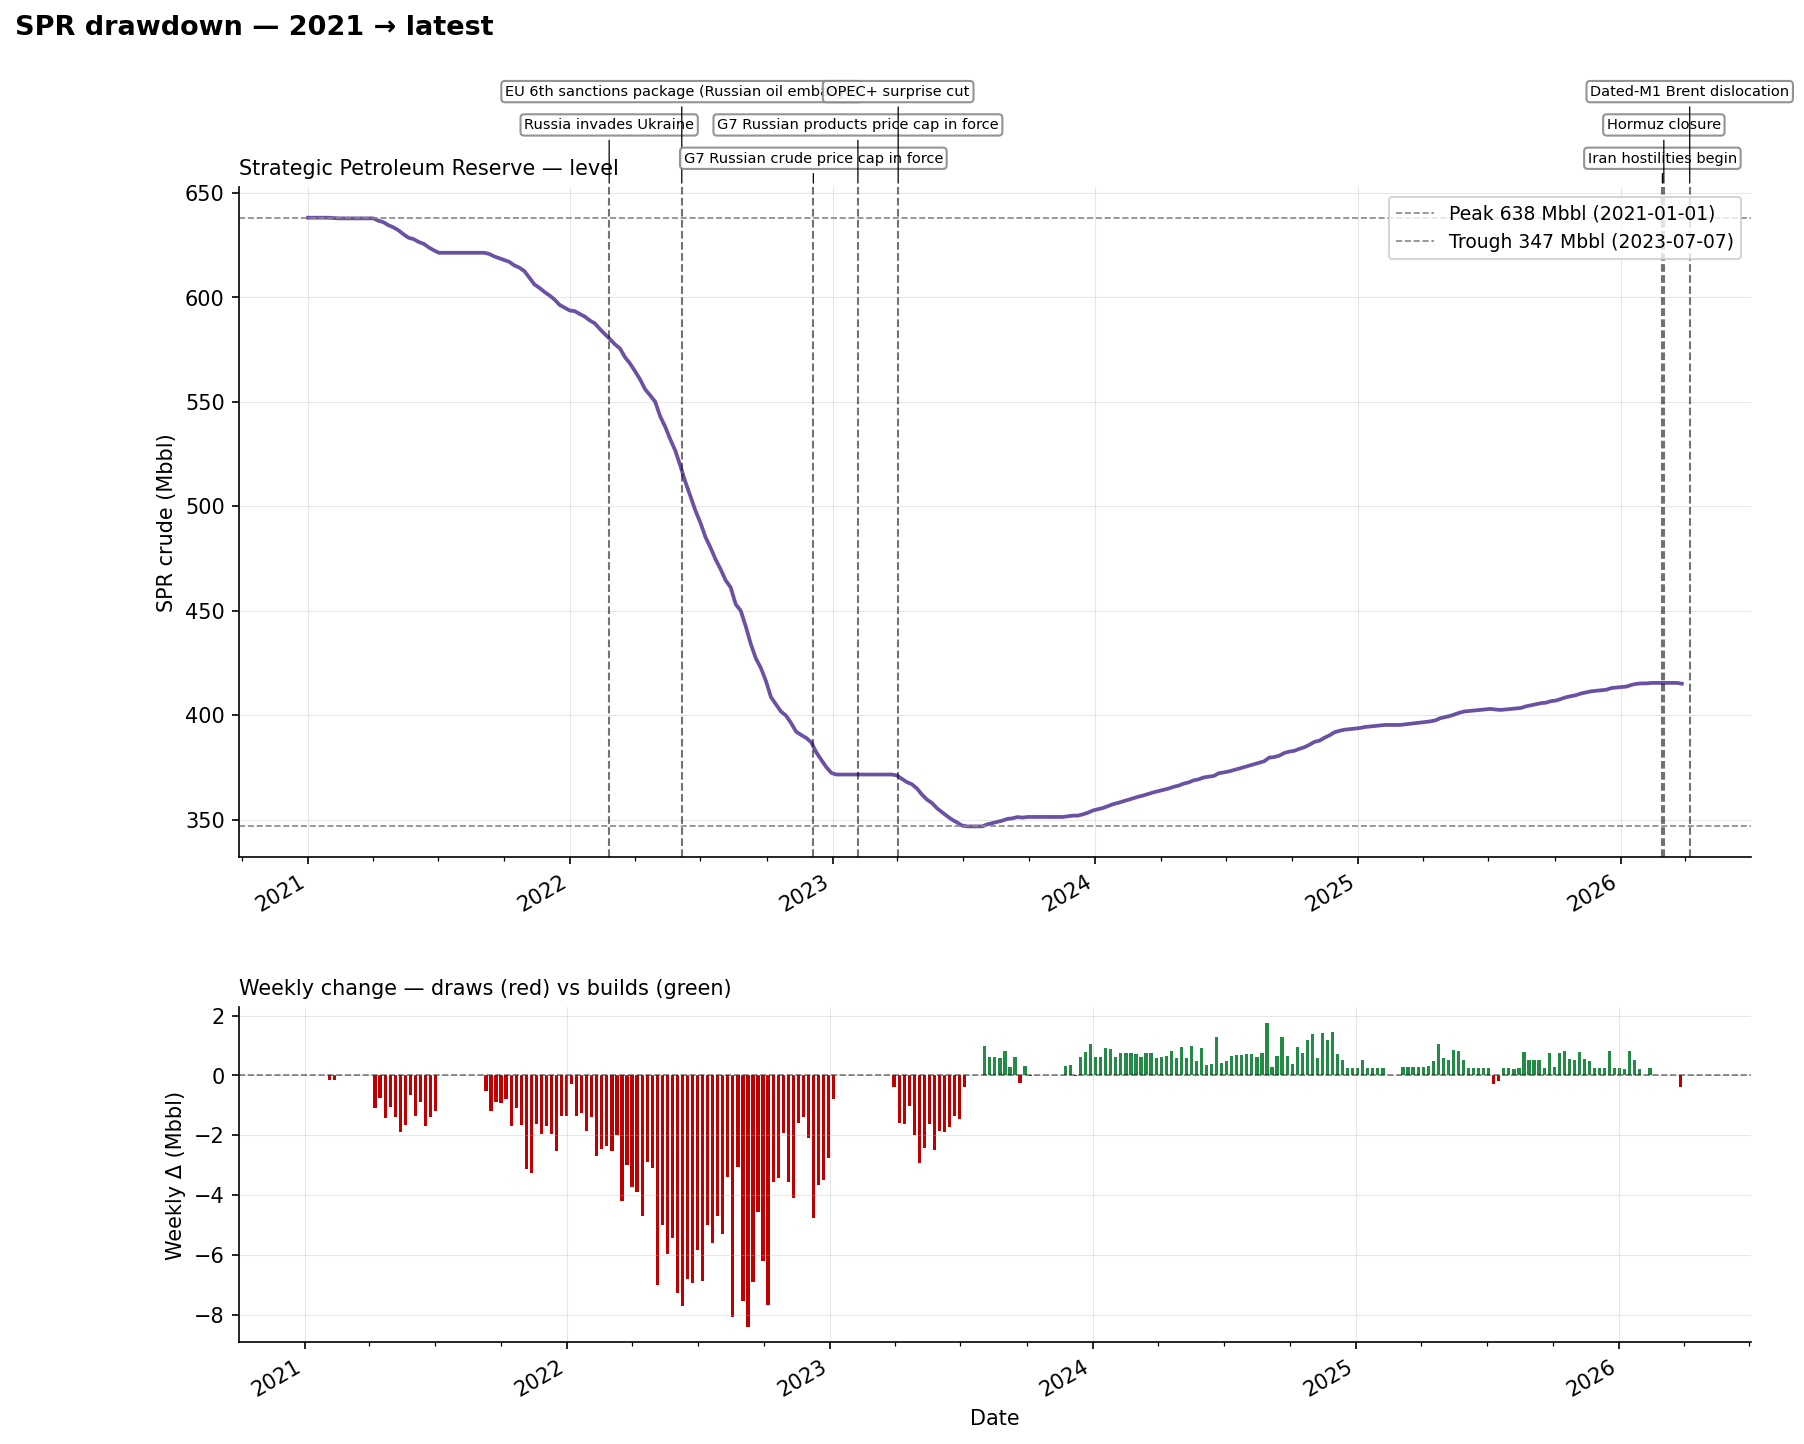
\includegraphics[width=\linewidth]{fig_07b_spr.png}\\[0.2cm]
{\footnotesize\textit{SPR drawdown since 2021.}}
\end{center}

\end{minipage}

\vspace{0.3cm}
%% [trailing bridge removed for pagination]

\newpage

% ============================================================================
% SECTION 8 — FUNDAMENTALS II
% ============================================================================
\section{US yields and EU refinery runs: the response that didn't come}\label{sec:8}

\textit{The textbook slate swing never happened, so the diesel crack has to clear through price or imports.}

\noindent\textcolor{obred}{\textbf{Desk decision.}} \emph{No yield-mix swing means the diesel crack won't compress on supply response. It clears through price (long ULSD crack) or imports (USG / India / AG flow geometry).}

\vspace{0.2cm}

\noindent\begin{minipage}[t]{0.48\linewidth}\vspace{0pt}

When a refinery sees the diesel crack widen and the gasoline crack stay flat, the textbook response is to swing the slate, re-tune hydrocrackers, shift cut points, put more of each barrel into the more valuable product. In the data, that swing would show up as a rising distillate tilt, the gap between distillate yield and gasoline yield.

US yields have been flat. The distillate tilt has sat near \textbf{$-17$ pp} all the way through 2025 and into 2026, which is no different from the pre-crisis average. Refiners haven't structurally moved toward diesel despite the margin signal. Two possible reads: either the squeeze is seen as short-lived (and hydrocracker retuning isn't worth the operational cost for a few weeks of premium), or the system is already at its max-distillate cutpoint given its crude diet. Either way, the supply response from yield mix isn't coming, and the crack has to clear through price or through imports.

EU refinery intake holds up decently. Germany, Netherlands, Italy, France and Spain carry the line, with total runs around 50-55 Mt/month and the usual 12-month seasonal cycle. The recent months print below the 12-month MA, which fits the story of margin-driven run cuts plus crude-supply disruption in the Med.

One operational note: trailing months with fewer than 10 reporting countries are dropped from the chart. Eurostat publishes with a 2-3 month lag, and the most recent couple of months usually have only 1-2 early filers.

\end{minipage}\hfill
\begin{minipage}[t]{0.48\linewidth}\vspace{0pt}

\begin{center}
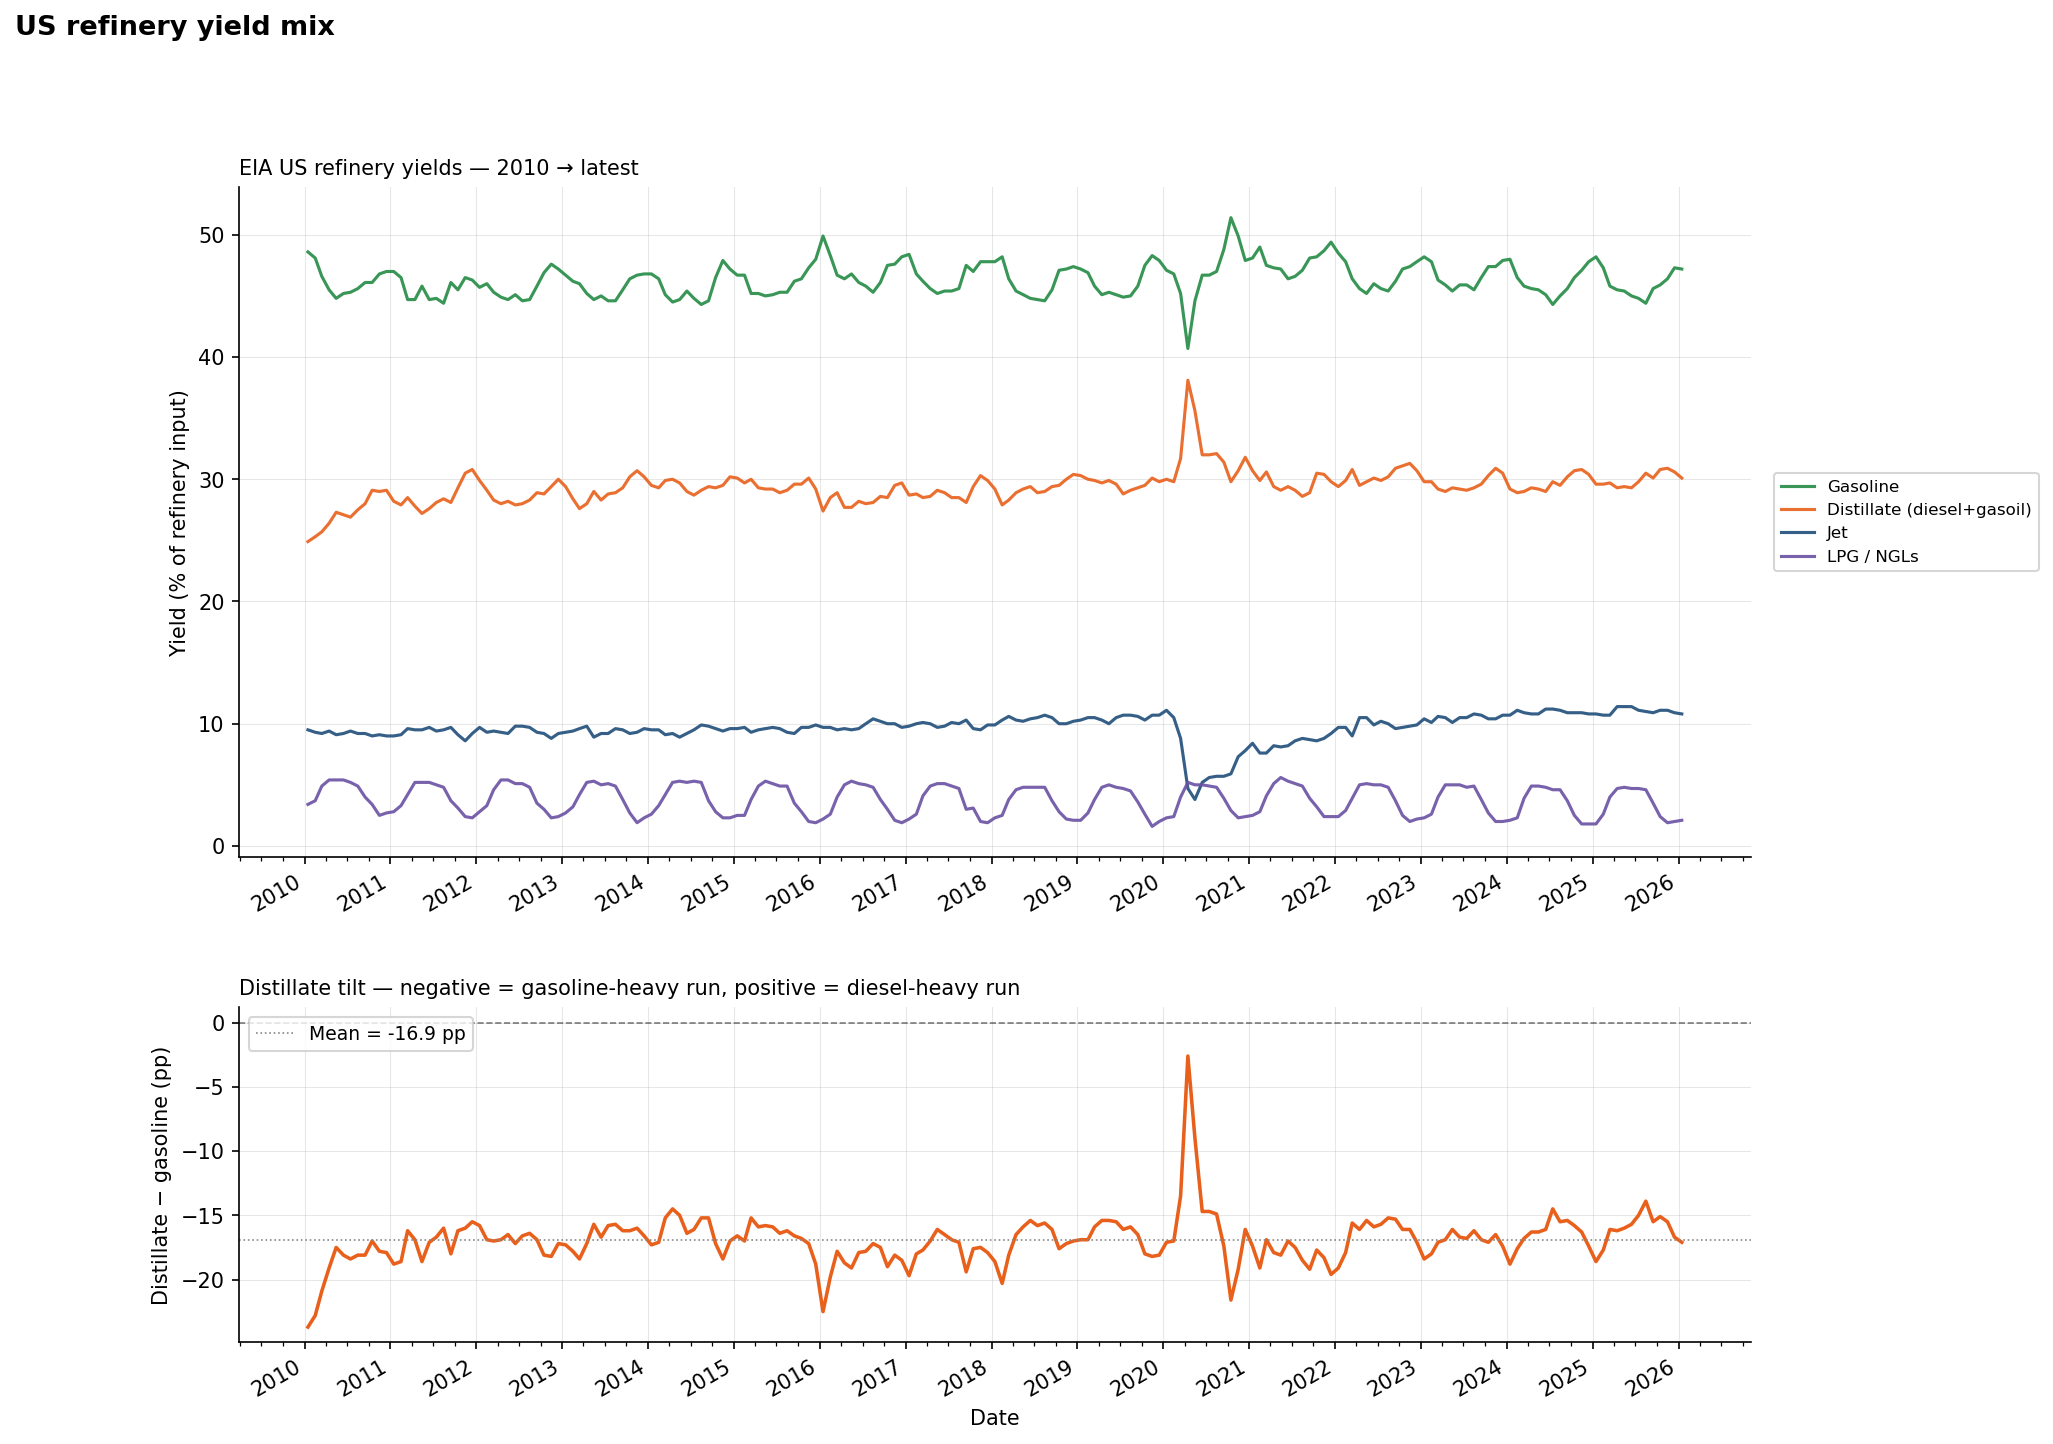
\includegraphics[width=\linewidth]{fig_08a_us_yields.png}\\[0.2cm]
{\footnotesize\textit{US refinery yields, 2010+. Distillate tilt hasn't moved.}}
\end{center}

\vspace{0.2cm}

\begin{center}
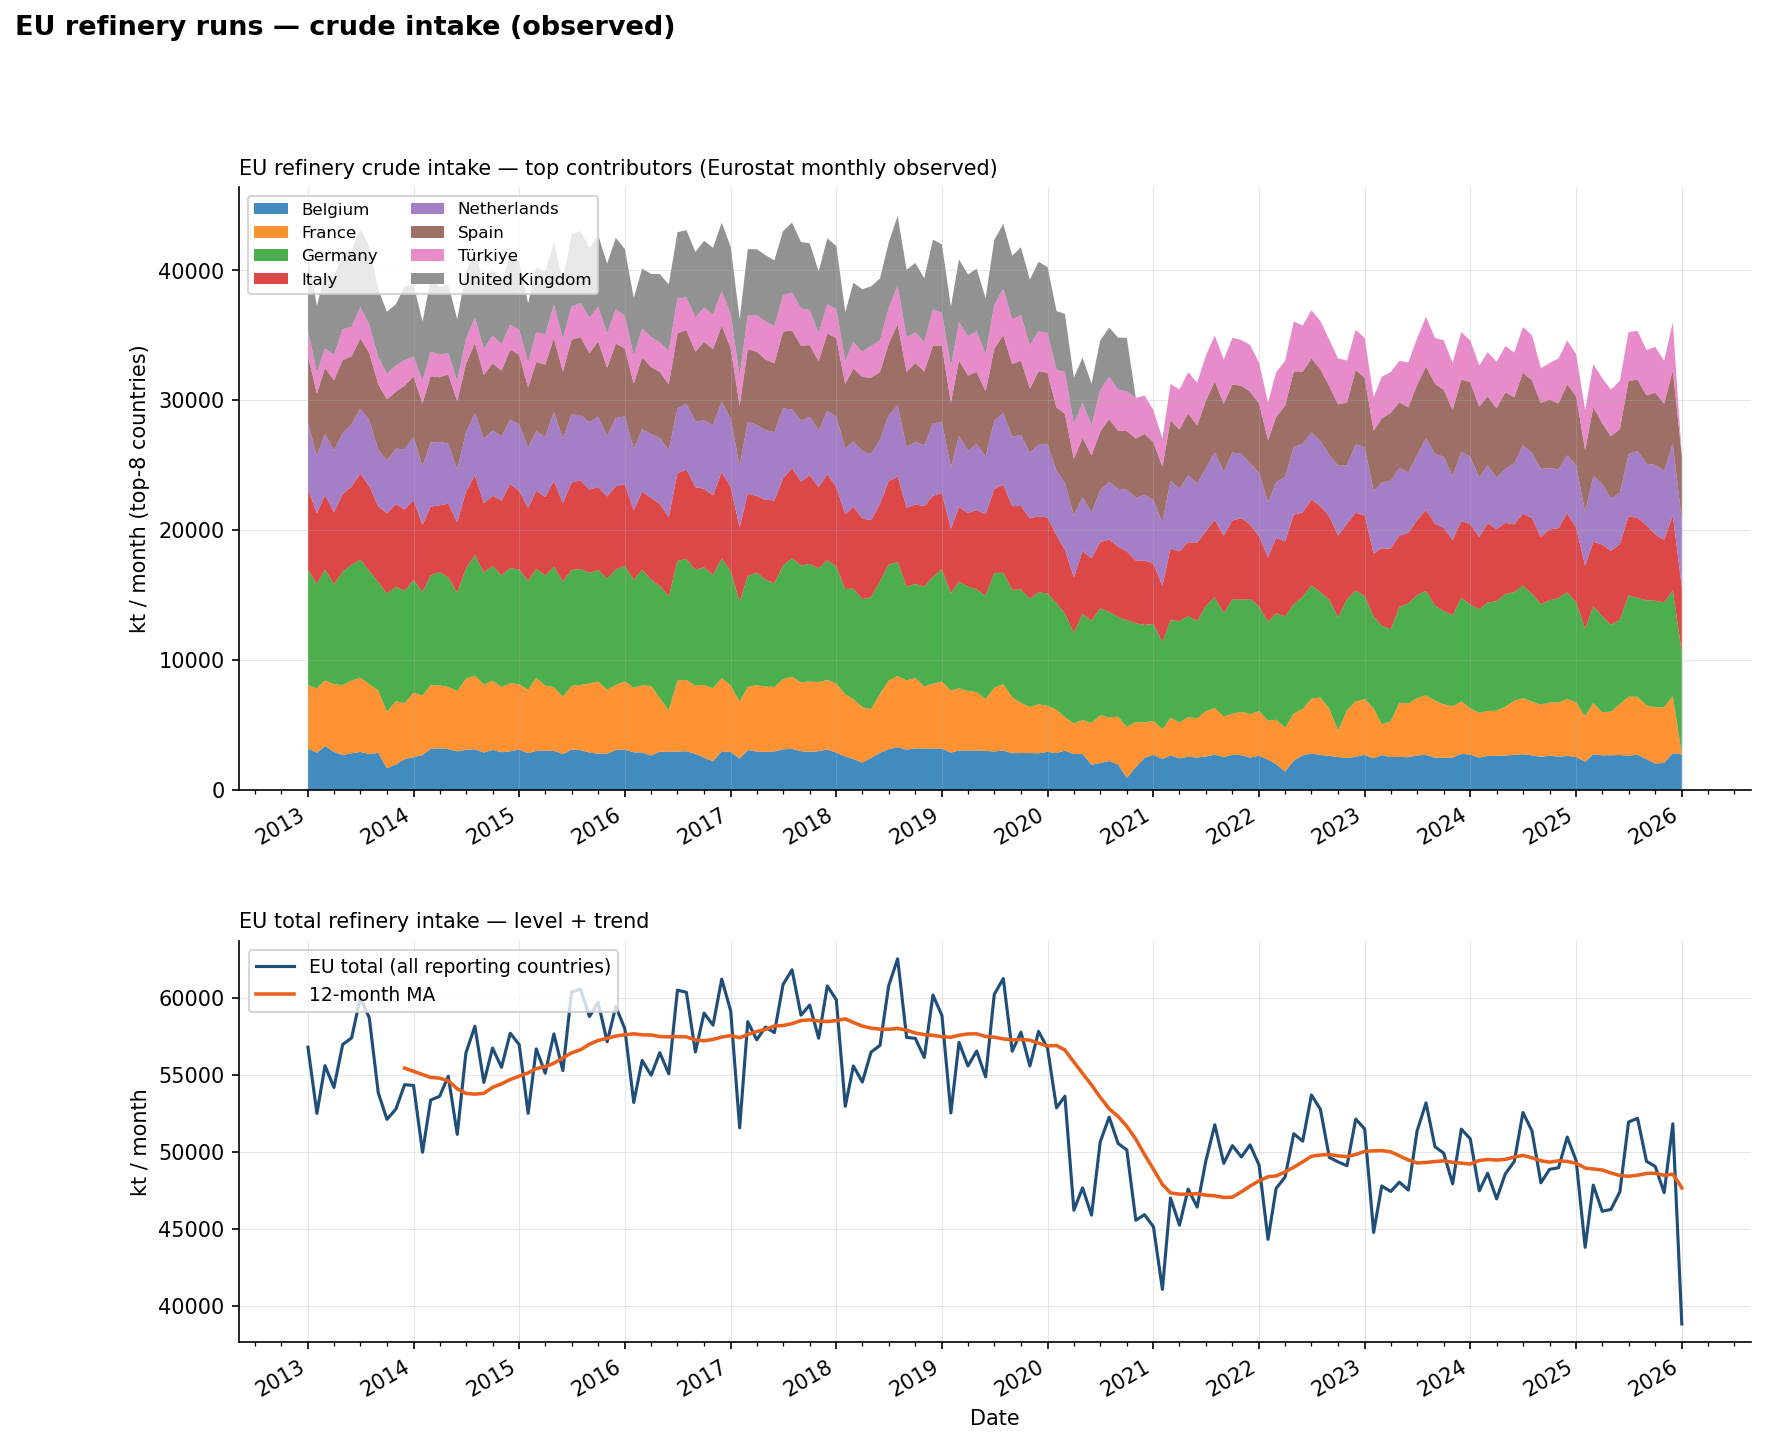
\includegraphics[width=\linewidth]{fig_08b_eu_intake.png}\\[0.2cm]
{\footnotesize\textit{EU refinery crude intake, top-8 countries stacked, 12-month MA on the total.}}
\end{center}

\end{minipage}

\vspace{0.3cm}
%% [trailing bridge removed for pagination]

\newpage

% ============================================================================
% SECTION 9 — FUNDAMENTALS III
% ============================================================================
\section{The EU diesel deficit, annualised}\label{sec:9}

\textit{One structural number sets the whole price level for \mbox{NWE} ULSD.}

\noindent\textcolor{obred}{\textbf{Desk decision.}} \emph{EU27 is structurally short $\sim$29 Mt/y diesel; imports set the marginal price. NWE ULSD crack \emph{is} the EU-deficit clearing price --- this is why it decouples from WTI-anchored paper cracks under stress.}

\vspace{0.2cm}

\noindent\begin{minipage}[t]{0.45\linewidth}\vspace{0pt}

The single structural number that explains most of what happens in the \mbox{NWE} ULSD crack.

\begin{center}
\bignum{$\approx$ 29 Mt/year}{EU27 diesel import dependence (Eurostat \texttt{nrg\_cb\_oilm}, post-2020 perimeter), pooled 2018--2026 average. \emph{+UK adds $\approx$ 8--10 Mt/y on pre-2021 figures; UK leaves Eurostat after Dec-2020 (Brexit perimeter), so this is a 2018--2020 average projected forward, not live.}}
\end{center}

\vspace{0.2cm}

Consumption (Eurostat gross inland deliveries) minus EU refinery output averages roughly +2,400 kt/month of deficit. Europe imports that gap via USGC, India, Arab Gulf, and the Russia shadow fleet post-sanctions. Because that imported barrel is what clears the balance, it's also what sets \mbox{NWE} ULSD pricing. This is why \mbox{NWE} can decouple from \mbox{WTI}-anchored paper cracks in stress windows, and why the Med $\rightarrow$ \mbox{NWE} arb inversion showing in the Apr-24 Platts European Marketscan ($\Delta$Med-NWE +\$15.50/mt, AAWYZ00 vs AAVBG00) is a real signal rather than a data quirk.

The post-2022 annual number is higher than the pooled 29 Mt, because the price-cap regime cut some legacy Russian supply channels without fully closing them. Looking at the annual chart on the right, the deficit widened materially in 2022-2024 and stayed wide through 2025-2026.

The mechanism is simple: structural EU demand for diesel meets a refinery system that doesn't produce enough, and the gap has historically been cleared by replacement barrels from USGC, India, AG and Russia. Since 2022, the price cap removed Russia as a routine source for G7-linked buyers; since February 2026, Hormuz disruption put 3.8 mb/d of AG loadings into question. The chronic import need is now meeting a narrower set of actual suppliers, and the clearing mechanism is price.

\end{minipage}\hfill
\begin{minipage}[t]{0.53\linewidth}\vspace{0pt}

\begin{center}
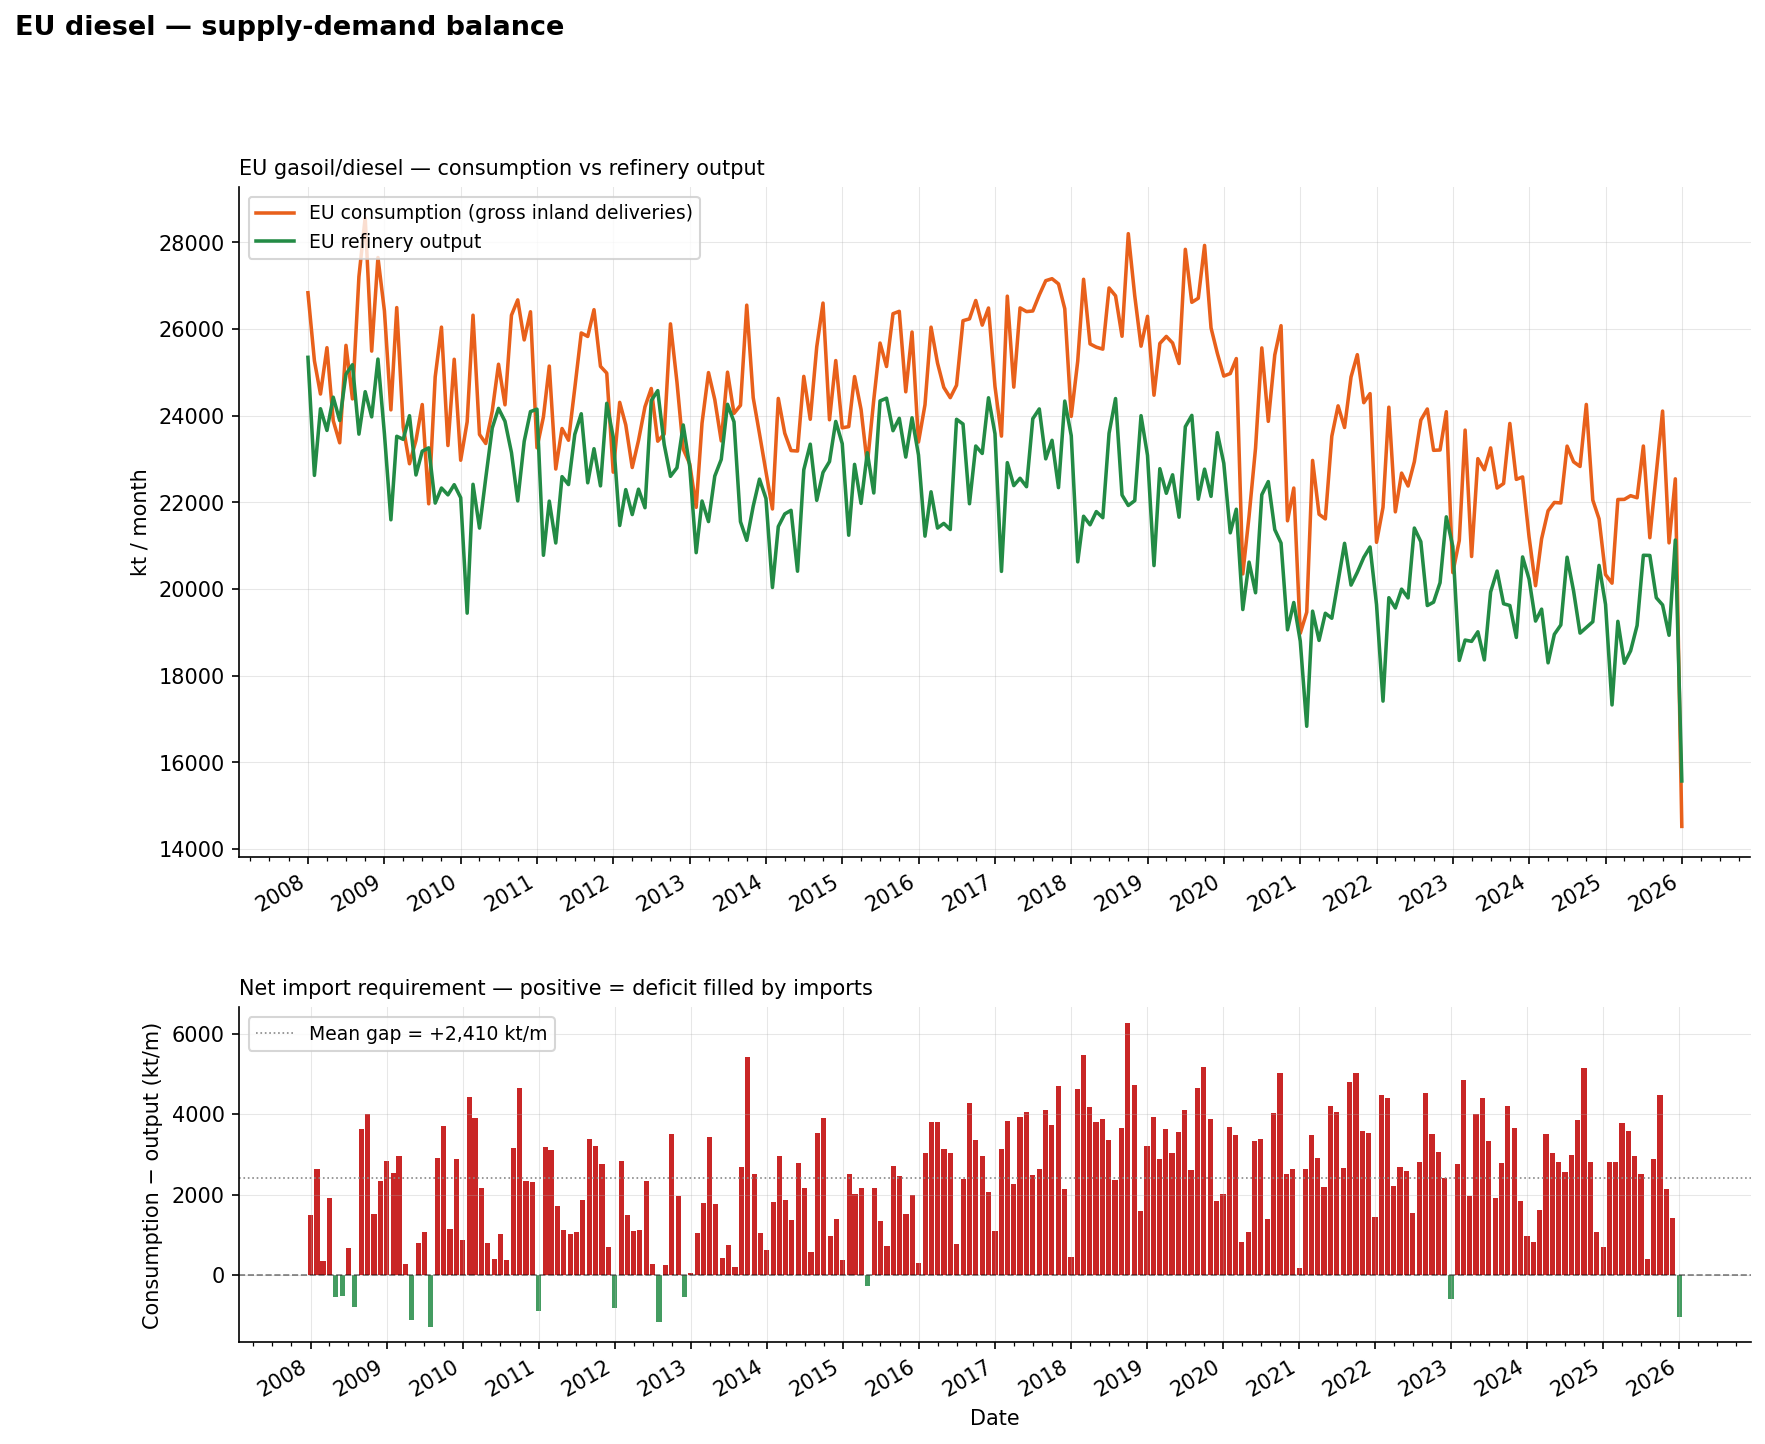
\includegraphics[width=\linewidth]{fig_09a_eu_consumption.png}\\[0.2cm]
{\footnotesize\textit{EU diesel --- consumption in orange, refinery output in green, deficit (consumption minus output) in the lower panel.}}
\end{center}

\vspace{0.2cm}

\begin{center}
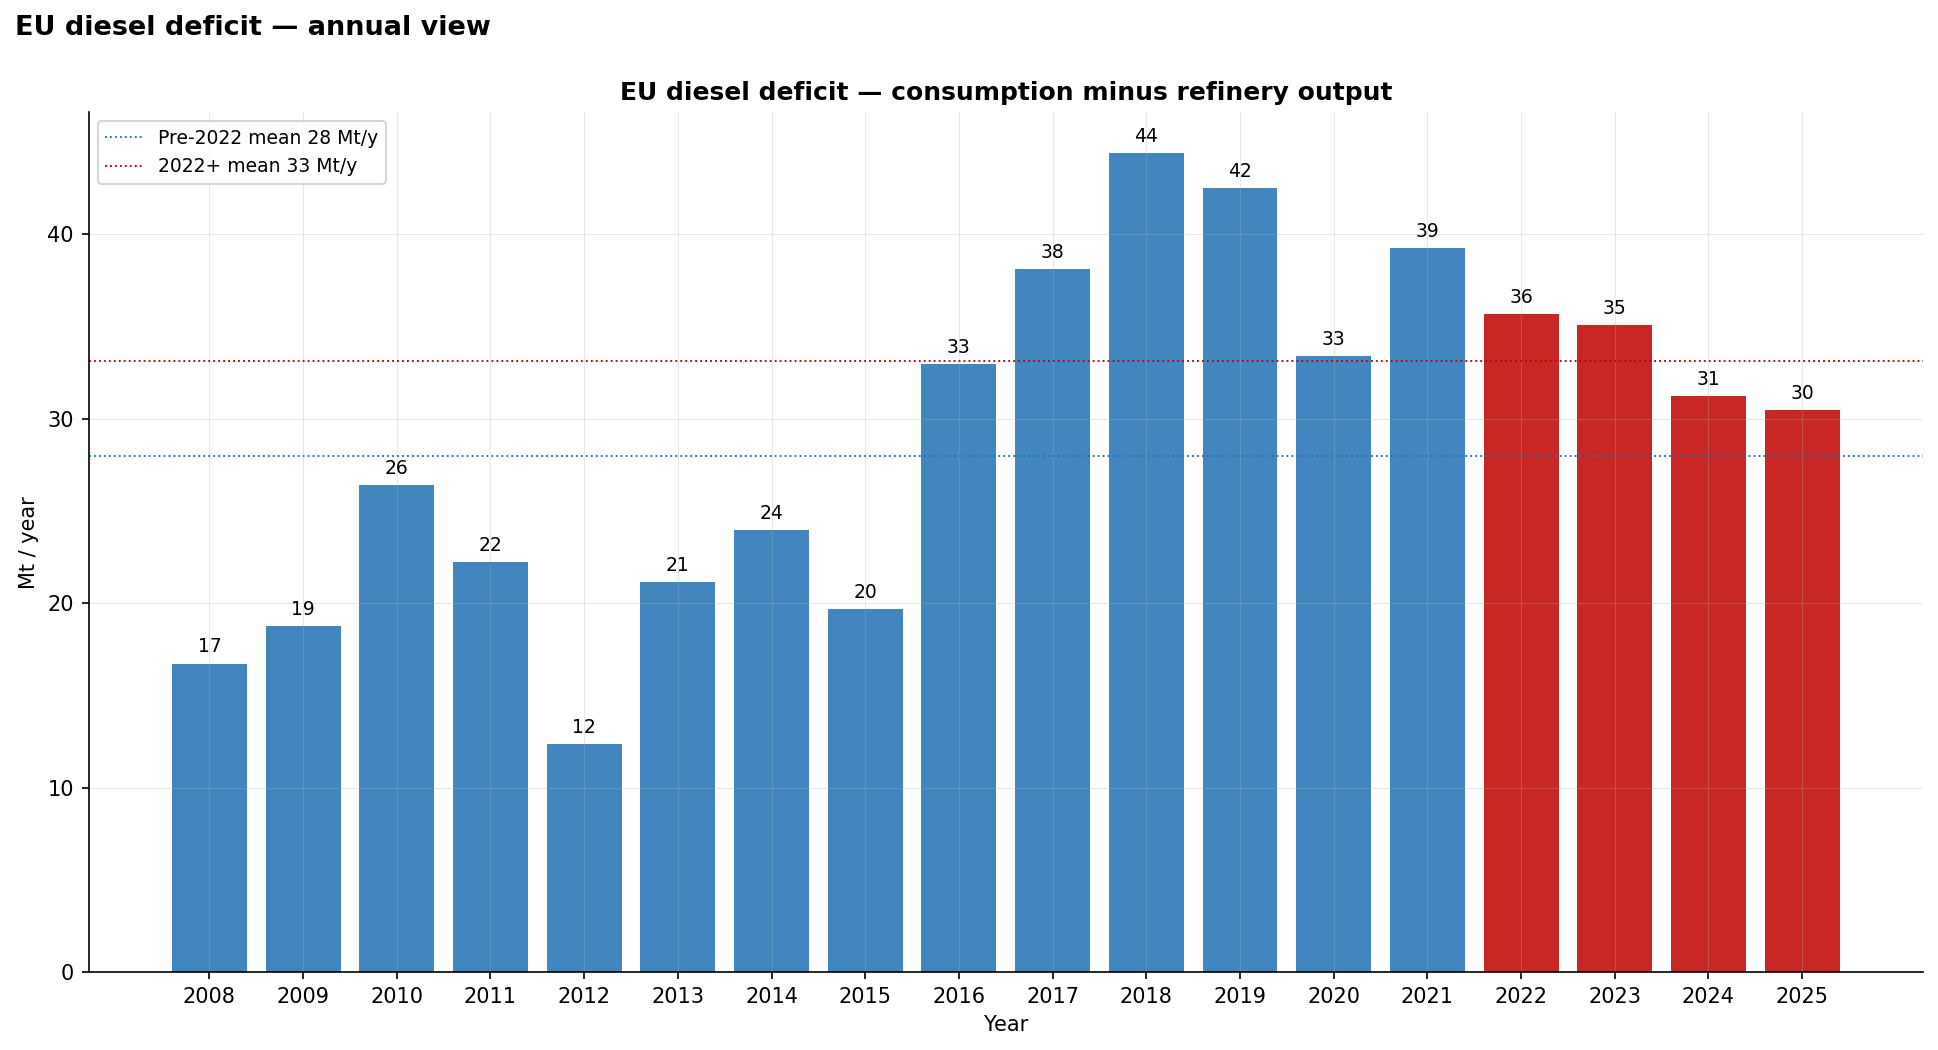
\includegraphics[width=\linewidth]{fig_09c_eu_deficit_annual.png}\\[0.2cm]
{\footnotesize\textit{Annual EU deficit, blue bars pre-2022, red 2022+. The post-2022 mean step-changes clearly above the pooled 29 Mt figure.}}
\end{center}

\end{minipage}

\vspace{0.3cm}
%% [trailing bridge removed for pagination]

\newpage

% ============================================================================
% SECTION 10 — FLOWS
% ============================================================================


\section{Flows: where Russian barrels ended up, where OPEC exports live}\label{sec:10}

\textit{The physical map of which countries fill Europe's diesel gap, and at what freight cost.}

\noindent\textcolor{obred}{\textbf{Desk decision.}} \emph{Replacement supply (USGC + India + AG + WAF) is what clears Europe; direct Russia-to-Europe is no longer the input. A single CIF NWE print resets the global product balance with a 2-week voyage-time lag.}

\vspace{0.2cm}

\noindent\begin{minipage}[t]{0.50\linewidth}\vspace{0pt}

Russian diesel post-price-cap: the flow didn't die, it rerouted. Turkey, Brazil, and the Middle East dominate destinations. Russian barrels are still in the global pool, they're just not reaching Europe. For a desk trading the \mbox{NWE} crack, that means the replacement supply, USGC, India, AG, WAF, is what clears the Europe balance and sets \mbox{NWE} price. Direct Russia-to-Europe flows aren't the input anymore.

\vspace{0.15cm}

EU diesel imports are diversified. No single origin dominates post-2022. That's a source of resilience (if one origin drops out, others can absorb) but it also means every shift in arb economics rebalances the mix. USGC had a big share when the Atlantic basin arb was open, India and AG took share when that arb closed, WAF's share moves with Dangote's Nigerian refinery ramp.

\end{minipage}\hfill
\begin{minipage}[t]{0.48\linewidth}\vspace{0pt}
\centerline{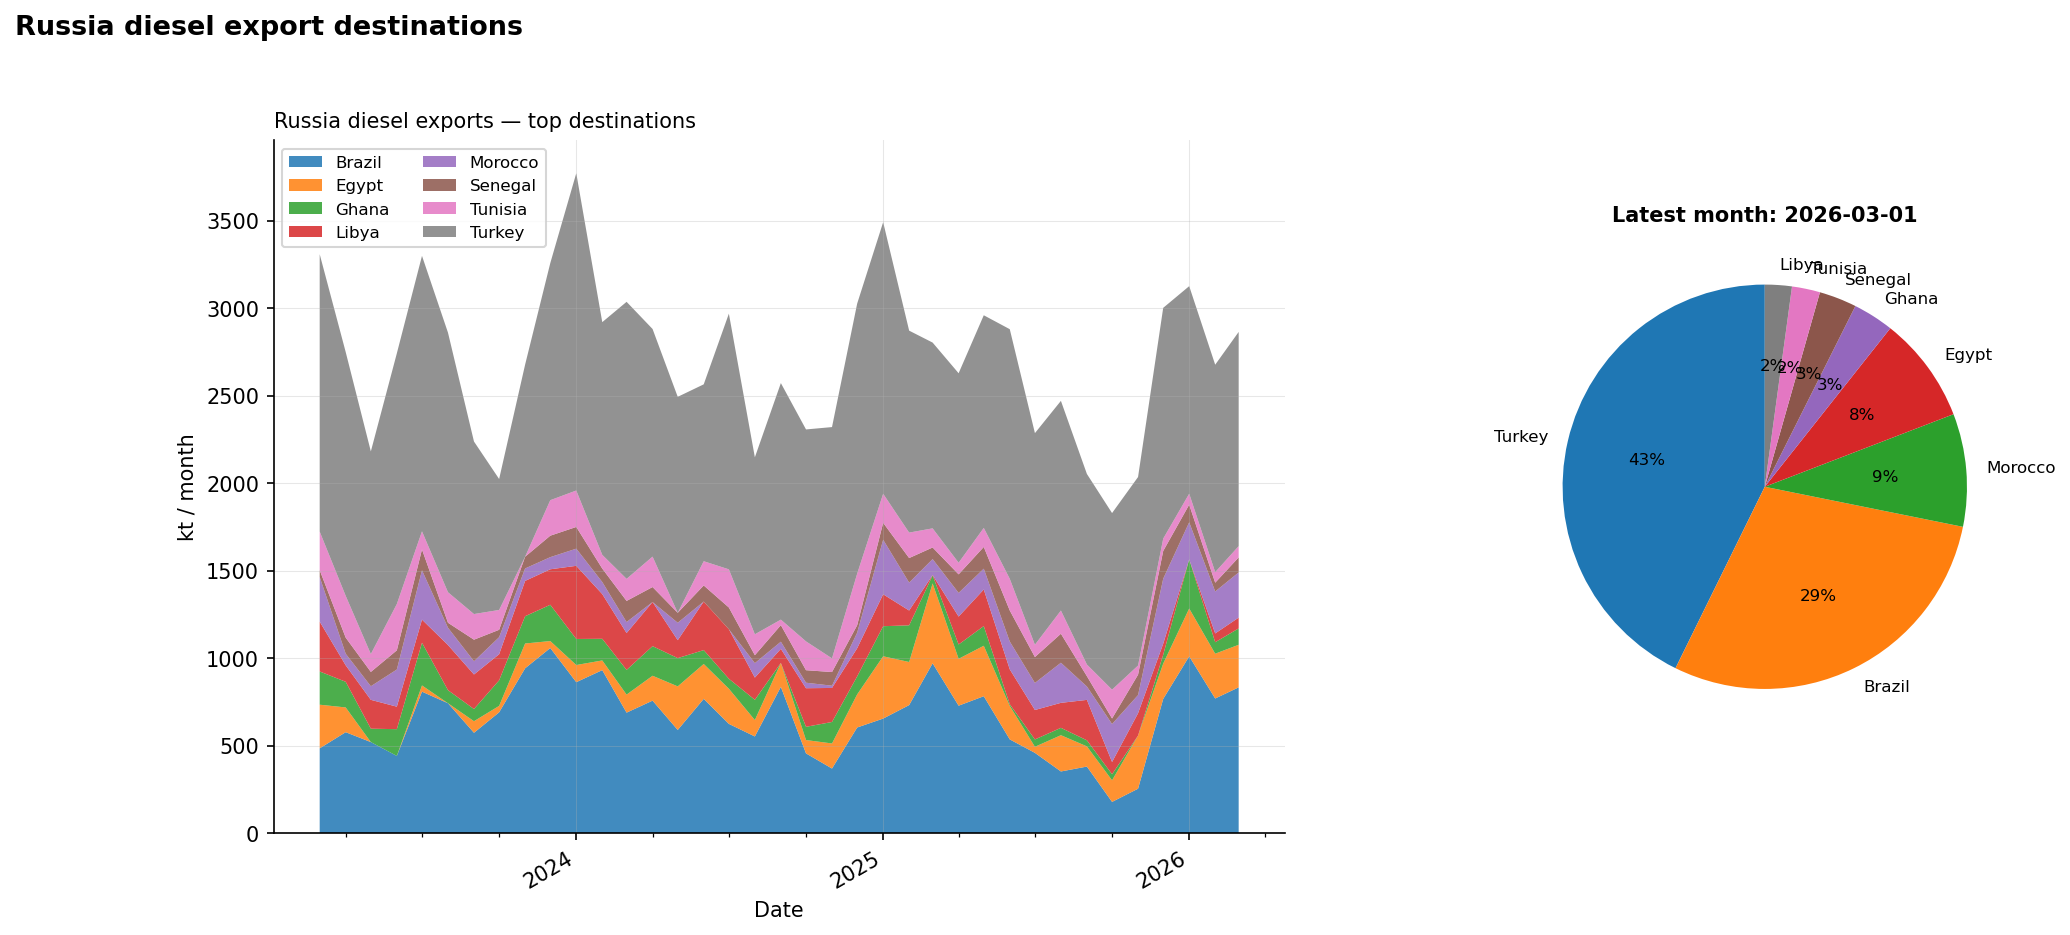
\includegraphics[width=\linewidth]{fig_10a_russia_export.png}}
{\footnotesize\textit{Russia diesel exports by destination, latest Feb-2026 observation.}}
\end{minipage}

\vspace{0.3cm}

\begin{callout}[Cross-market linkages --- US/EU/Asia, why one CIF Med print moves three balances]
\footnotesize
\textbf{US} \emph{[LIVE]:} USGC ULSD export (AAXRV00 \$150.47/b) clears trans-Atlantic when CIF \mbox{NWE} (AAVBG00 \$173.49/b) covers freight. Ladder: USGC supply $\rightarrow$ Atlantic MR $\rightarrow$ \mbox{NWE} crack $\rightarrow$ Med inversion $\rightarrow$ AG freight $\rightarrow$ Brent. US is the \emph{flex barrel} on the global product balance.\\[2pt]
\textbf{EU} \emph{[STRUCTURAL]:} 29 Mt/y diesel deficit; lost Russian flows reshored to USGC + India + AG. Compliance gating cuts the addressable origin set, and freight at w400+ closes Med-NWE which forces \mbox{NWE} cracks higher to ration demand. \mbox{NWE} ULSD crack \emph{is} the EU-deficit clearing price.\\[2pt]
\textbf{Asia} \emph{[LIVE+STRUCTURAL]:} India (Reliance/Nayara) is the swing exporter; price-taker on AG crude, price-setter on Singapore product. China \emph{[LIVE]} just got Hengli sanctioned (Apr 24 OFAC) which trims its Iranian-crude appetite at the margin. Singapore 10ppm ULSD vs Tampa creates a freight-arb diamond: closes around w300 MR, opens above w500 (current freight).\\[2pt]
\textbf{Why this matters today.} A single AAVBG00 print resets: (i) US ULSD export pull, (ii) EU rationing requirement, (iii) Asian arb lane orientation. The cross-market loop is what prevents Med crack from collapsing on a Hormuz de-escalation alone --- US/Asia substitution kicks in only with a $\sim$2-week lag because of voyage time.
\end{callout}

\newpage



\noindent\begin{minipage}[t]{0.50\linewidth}\vspace{0pt}

OPEC ASB gives the structural background: US, Saudi and Russia dominate crude exports, and US product exports went from a footnote pre-2015-export-ban-repeal to the world's largest flow in under a decade. The country rankings haven't shifted dramatically in the last 10 years, but the US product-export share has grown materially.

\vspace{0.15cm}

Freight is the enabler. In the OPEC ASB annual series the 2022 invasion and 2024 Red Sea spikes are visible (\textit{data through 2024 only}; the 2026 Hormuz spike is \emph{not} in this dataset and is added on the chart only as a vertical event marker for context). The mechanism is ton-mile expansion: when Russian crude goes to Asia instead of Europe, or East-West cargoes Cape around instead of transiting Suez, average voyage distance rises and freight rates follow. For 2026 specifically, see Apr 24 Platts Tankerwire fixtures cited in \S\ref{sec:2}.

\end{minipage}\hfill
\begin{minipage}[t]{0.48\linewidth}\vspace{0pt}
\centerline{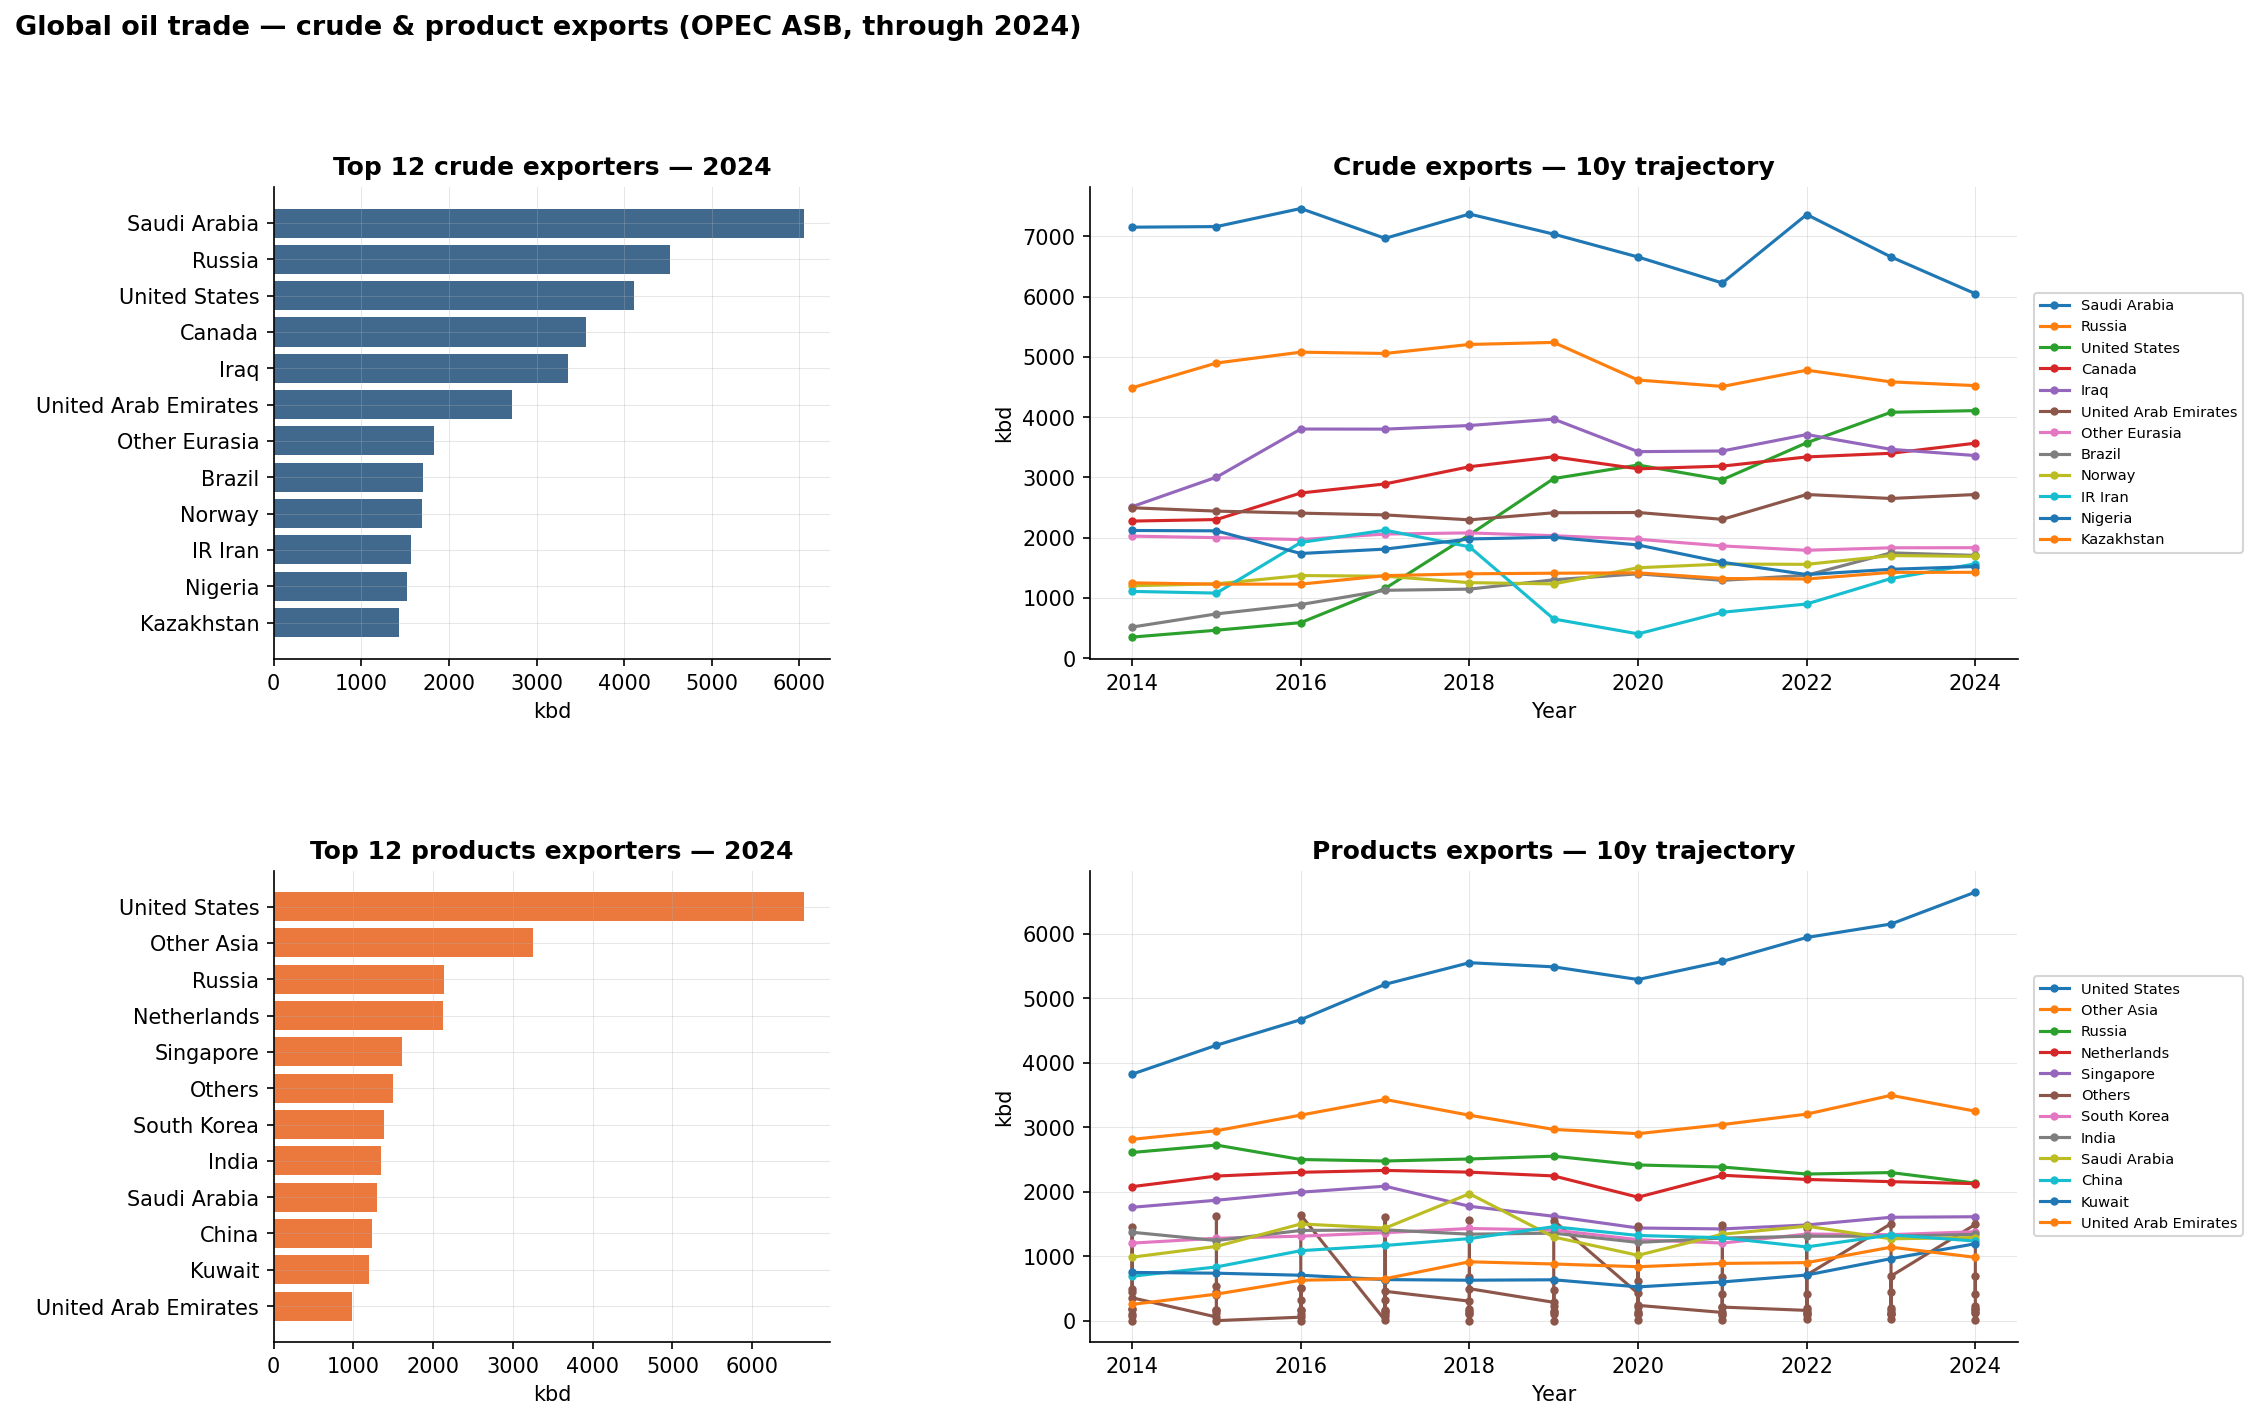
\includegraphics[width=\linewidth]{fig_10b_opec_trade.png}}
{\footnotesize\textit{OPEC ASB global crude and product exports, top-12 country trajectory, flows through 2024.}}
\end{minipage}

\vspace{0.4cm}

\begin{center}
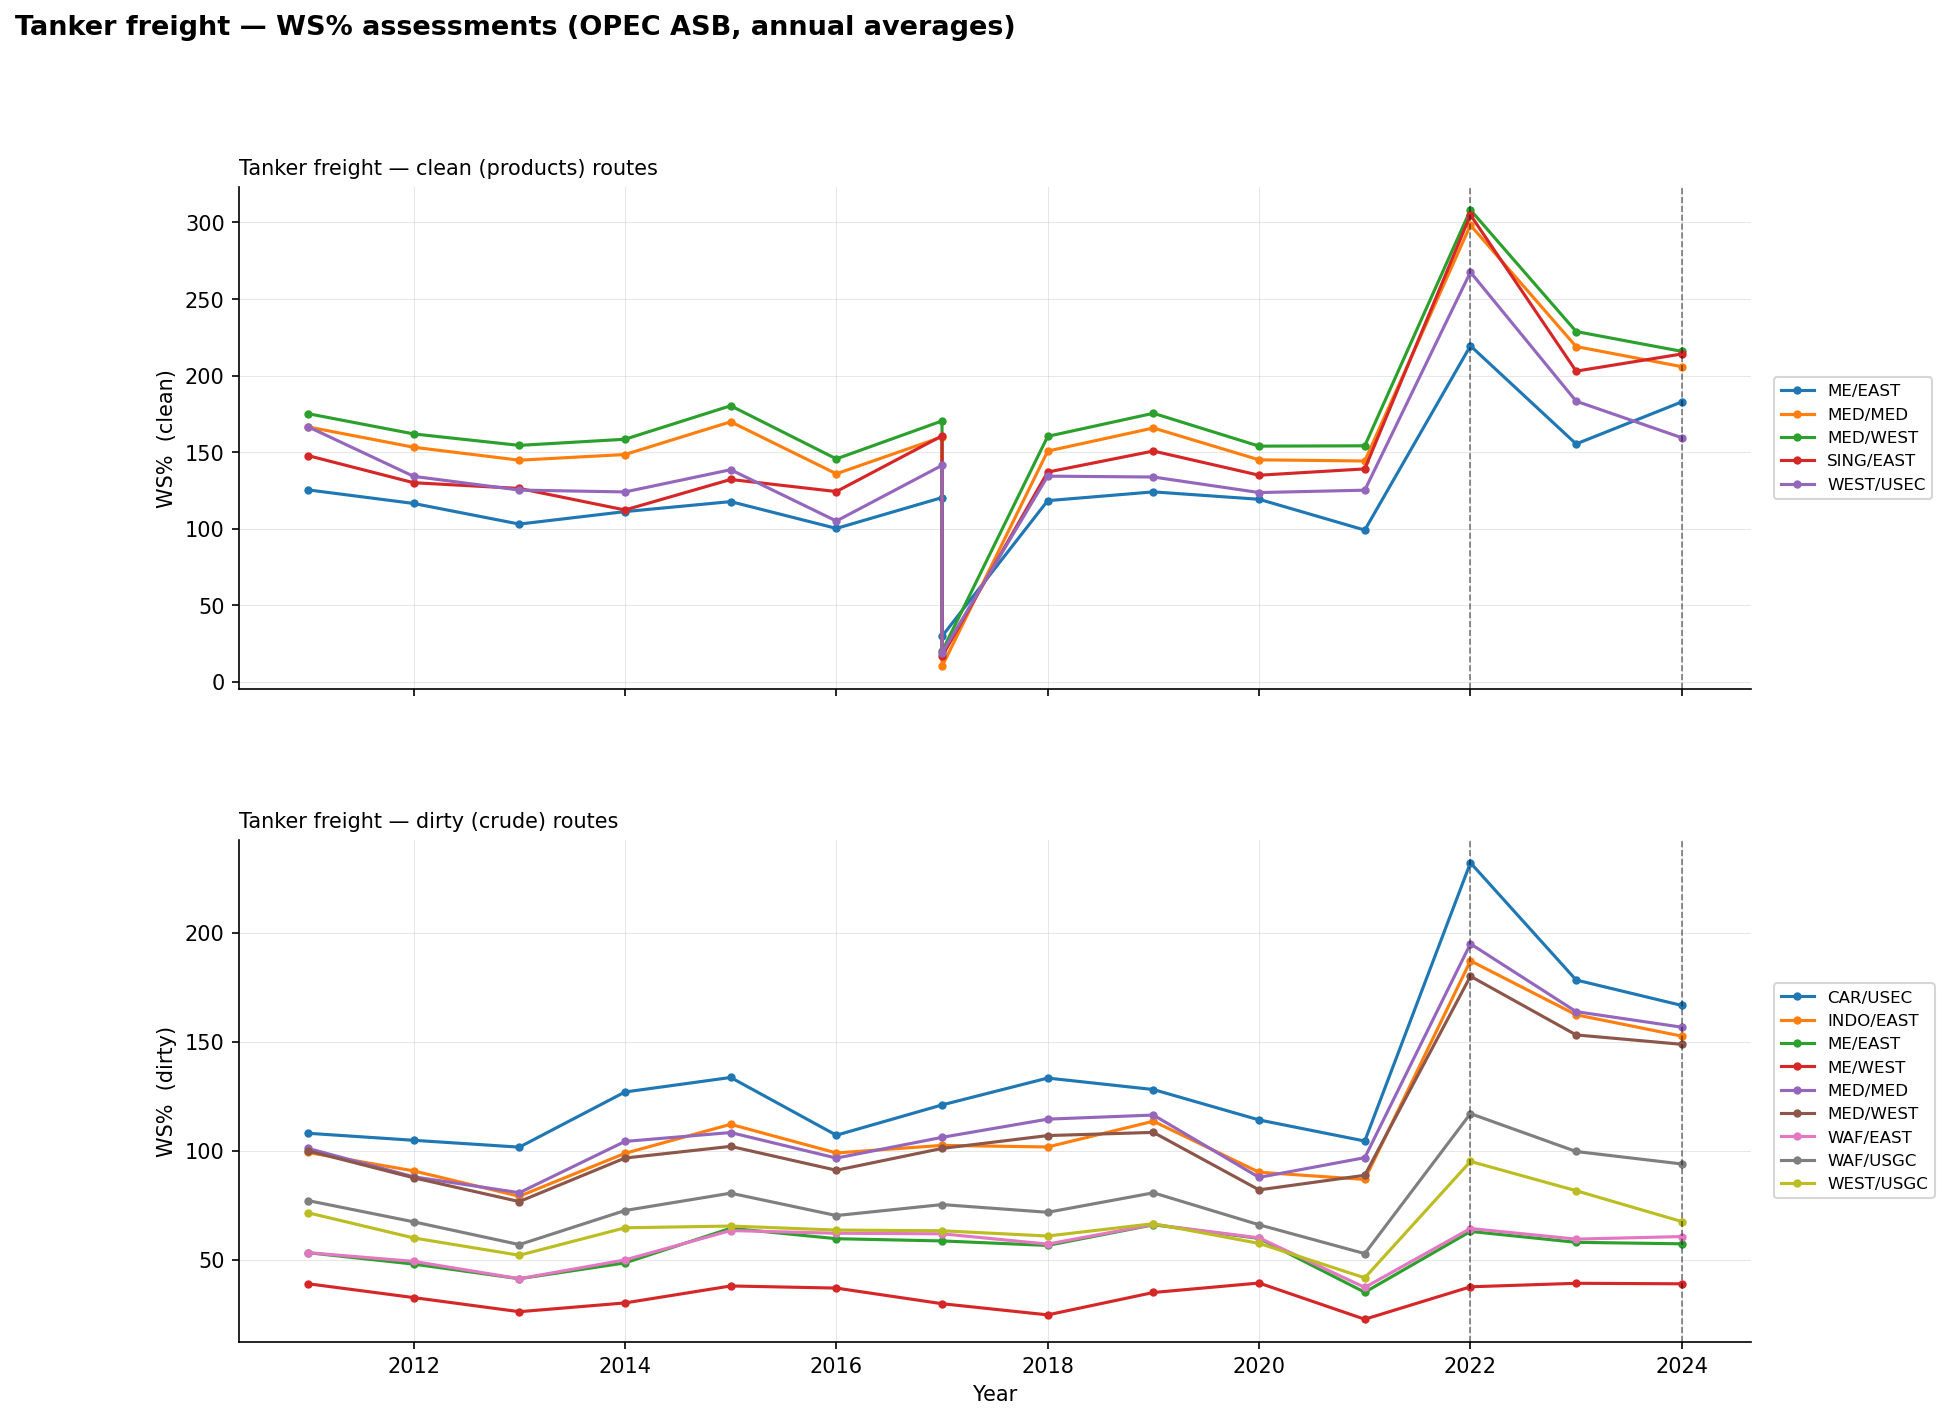
\includegraphics[width=0.88\linewidth]{fig_10c_opec_freight.png}\\[0.25cm]
\begin{minipage}{0.88\linewidth}
{\footnotesize\textit{OPEC ASB tanker freight, WS\% annual averages 2011--2024 (\textbf{data ends 2024}). 2022 invasion and 2024 Red Sea visible as data spikes; 2026 Hormuz shown as event-marker only --- live 2026 freight prints in \S\ref{sec:2} (Champion Arctic w405, Apr 24).}}
\end{minipage}
\end{center}

\newpage
\newpage

% ============================================================================
% SECTION 11 — ARB ENGINE
% ============================================================================
\section{Physical arbitrage engine: how the waterfall works}\label{sec:11}

\textit{A 9-item P\&L waterfall that turns any cargo decision into an executable net number.}

\noindent\textcolor{obred}{\textbf{Desk decision.}} \emph{Apr-24 USG$\rightarrow$NWE clears \textbf{+\$7.07/b arithmetically} at w405 freight, but is \textbf{operationally closed} for a generic G7 desk: needs \$10--12/b cushion + FFA + confirmed MR tonnage. Watchlist sub-200 reopener.}

\vspace{0.2cm}

\noindent\begin{minipage}[t]{0.46\linewidth}\vspace{0pt}

\texttt{CargoArb} takes any cargo decision and turns it into a nine-item P\&L waterfall. Gross spread in at the top; freight, port costs, canal tolls, financing, insurance, demurrage, broker commission all subtract; net arb comes out at the bottom.

The user picks the inputs: origin and destination ports from a dictionary, vessel class (MR, LR1, LR2, Aframax, Suezmax or VLCC), grade, cargo tonnage or capacity utilisation (under 1 for part-loaded cargoes), Worldscale rate, the two forward prices, and regional premium or discount on each side. Canal tolls, port costs, financing, demurrage and broker commission all come from the config's static tables.

Freight follows the standard Worldscale formula: \emph{freight = WS $\times$ flat rate / 100}. The grade's density (barrels per metric tonne) converts between MT and bbl, and voyage days come from distance divided by laden speed per vessel class.

As a calibration check, the engine reproduces a 2026-Q2 TD6-class Suezmax fixture (WS 230.56, flat 11.09) to the dollar: freight 25.57 USD/MT, cargo freight \$3.45 M on a 135 kMT parcel. If the Worldscale math is right, the rest of the waterfall at least has the freight line correct.

\textbf{Default lane.} The new default is \textbf{USG $\rightarrow$ \mbox{NWE} ULSD} on an MR tanker. The BSea $\rightarrow$ Med Aframax preset is tagged COMPLIANCE-GATED and carries the updated -\$15 Urals discount (post-price-cap narrowed), not the historical -\$30.

\textbf{Live freight, Apr 24, USG $\rightarrow$ \mbox{NWE} MR:} BP fixed the \emph{Champion Arctic} for a USGC-Transatlantic ULSD voyage at \textbf{w405} (Platts Clean Tankerwire). At TC2\_USG\_Continent flat \$24.50/mt $\times$ 4.05 = \$99.23/mt freight, on a 35--38 kt MR cargo, that is \$3.5--3.8 M cargo freight or roughly \$140--170 k/day TCE before bunkers. \textbf{The arb engine clears at +\$7.07/b net at this WS} (full waterfall below); the lane is \emph{arithmetically open, operationally closed} for a generic G7-linked desk --- vetting / credit / no-FFA gate the executable spread, not the freight math. The full-width waterfall and break-even logic below give the line-by-line build.

\textbf{Clearing vs executable.} The "open arithmetically" reading on a high-WS cargo is a clearing level, not an executable margin. Ops, compliance, and counterparty-vetting gates typically close most of what the arithmetic shows open. The waterfall quantifies the upper bound; the desk decides what the achievable bound is.\strut%

\end{minipage}%
\hfill%
\begin{minipage}[t]{0.50\linewidth}\vspace{0pt}

\begin{center}
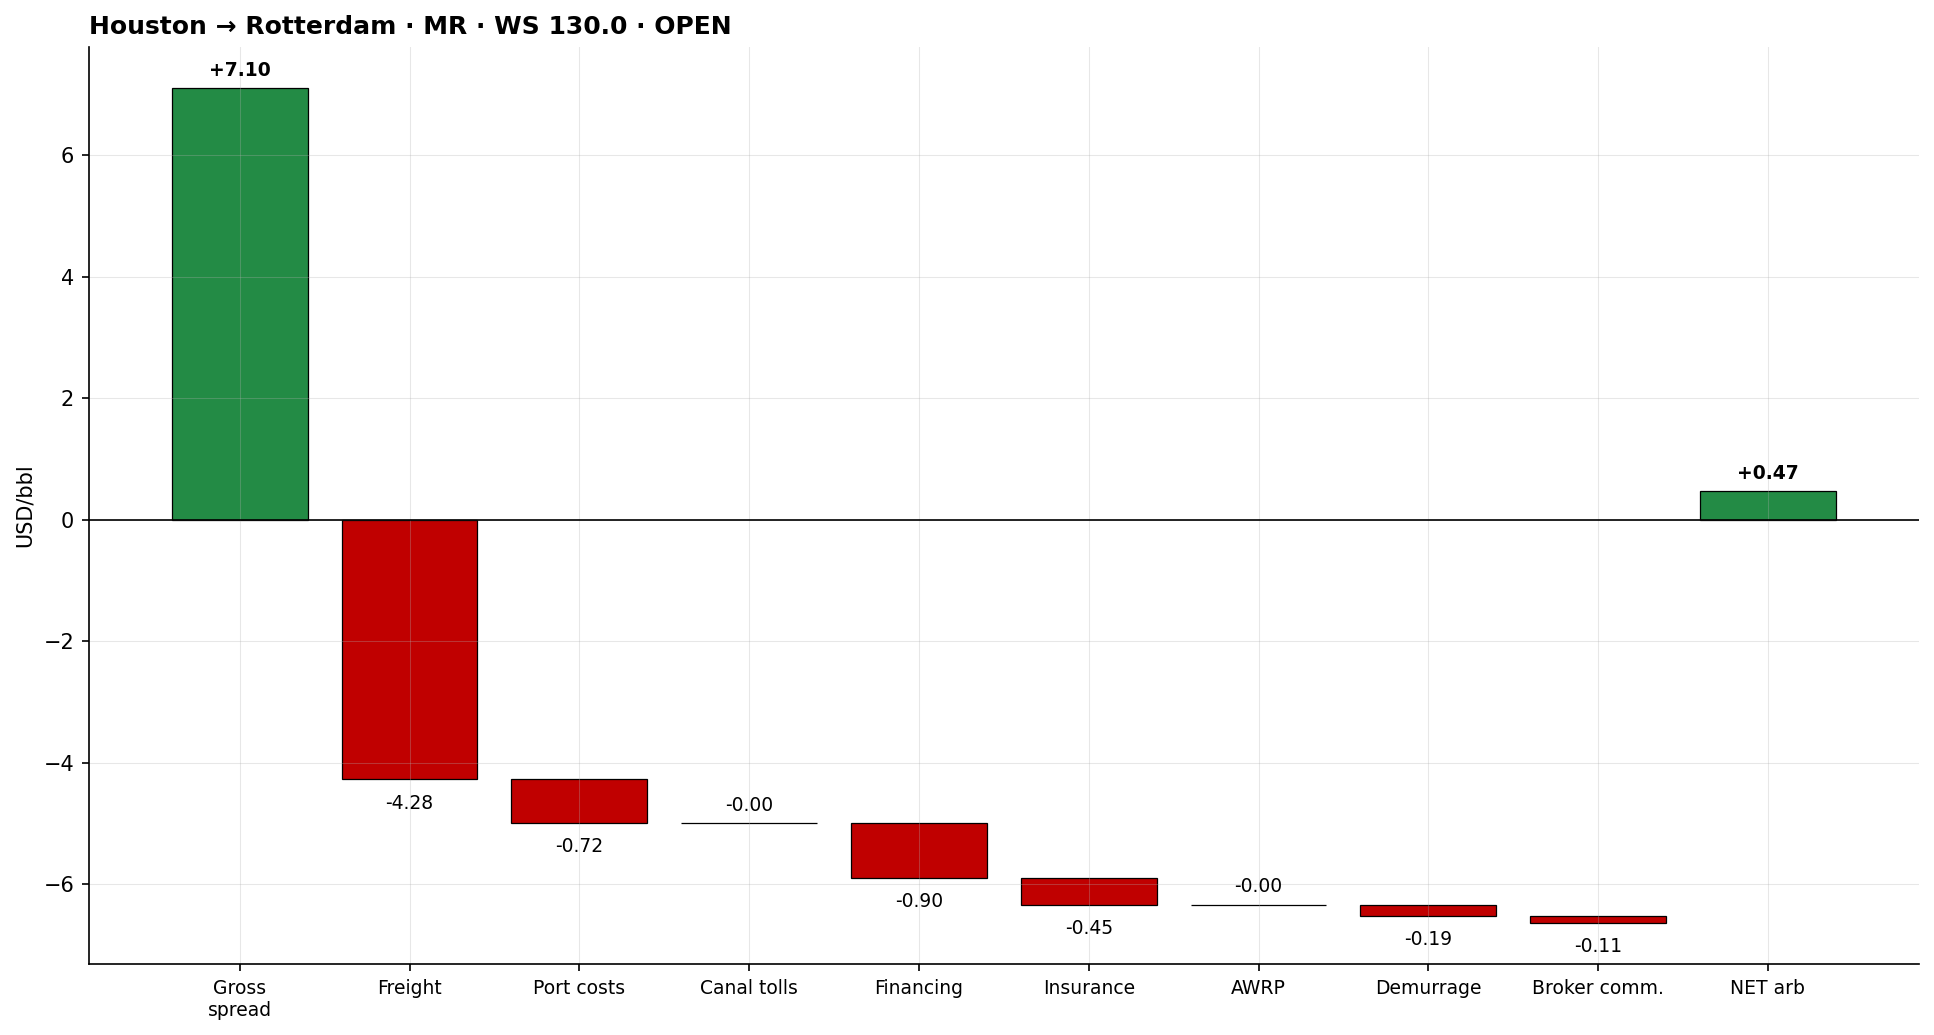
\includegraphics[width=\linewidth]{fig_11a_waterfall.png}\\[0.2cm]
{\footnotesize\textit{Default example: USG $\rightarrow$ \mbox{NWE} ULSD on an MR tanker. \textbf{Figure regenerated from a pre-Hormuz freight snapshot (WS $\sim$130).} At the Apr 24 fixture rate \textbf{w405} the live waterfall (below) clears \textbf{+\$7.07/b net} on a +\$23.02/b gross --- arithmetically open, but operationally closed for a generic G7 desk (vetting / credit / no-FFA). Visual kept to show waterfall structure; engine output for Apr 24 is in the body callout.}}
\end{center}

\vspace{0.2cm}

\begin{center}
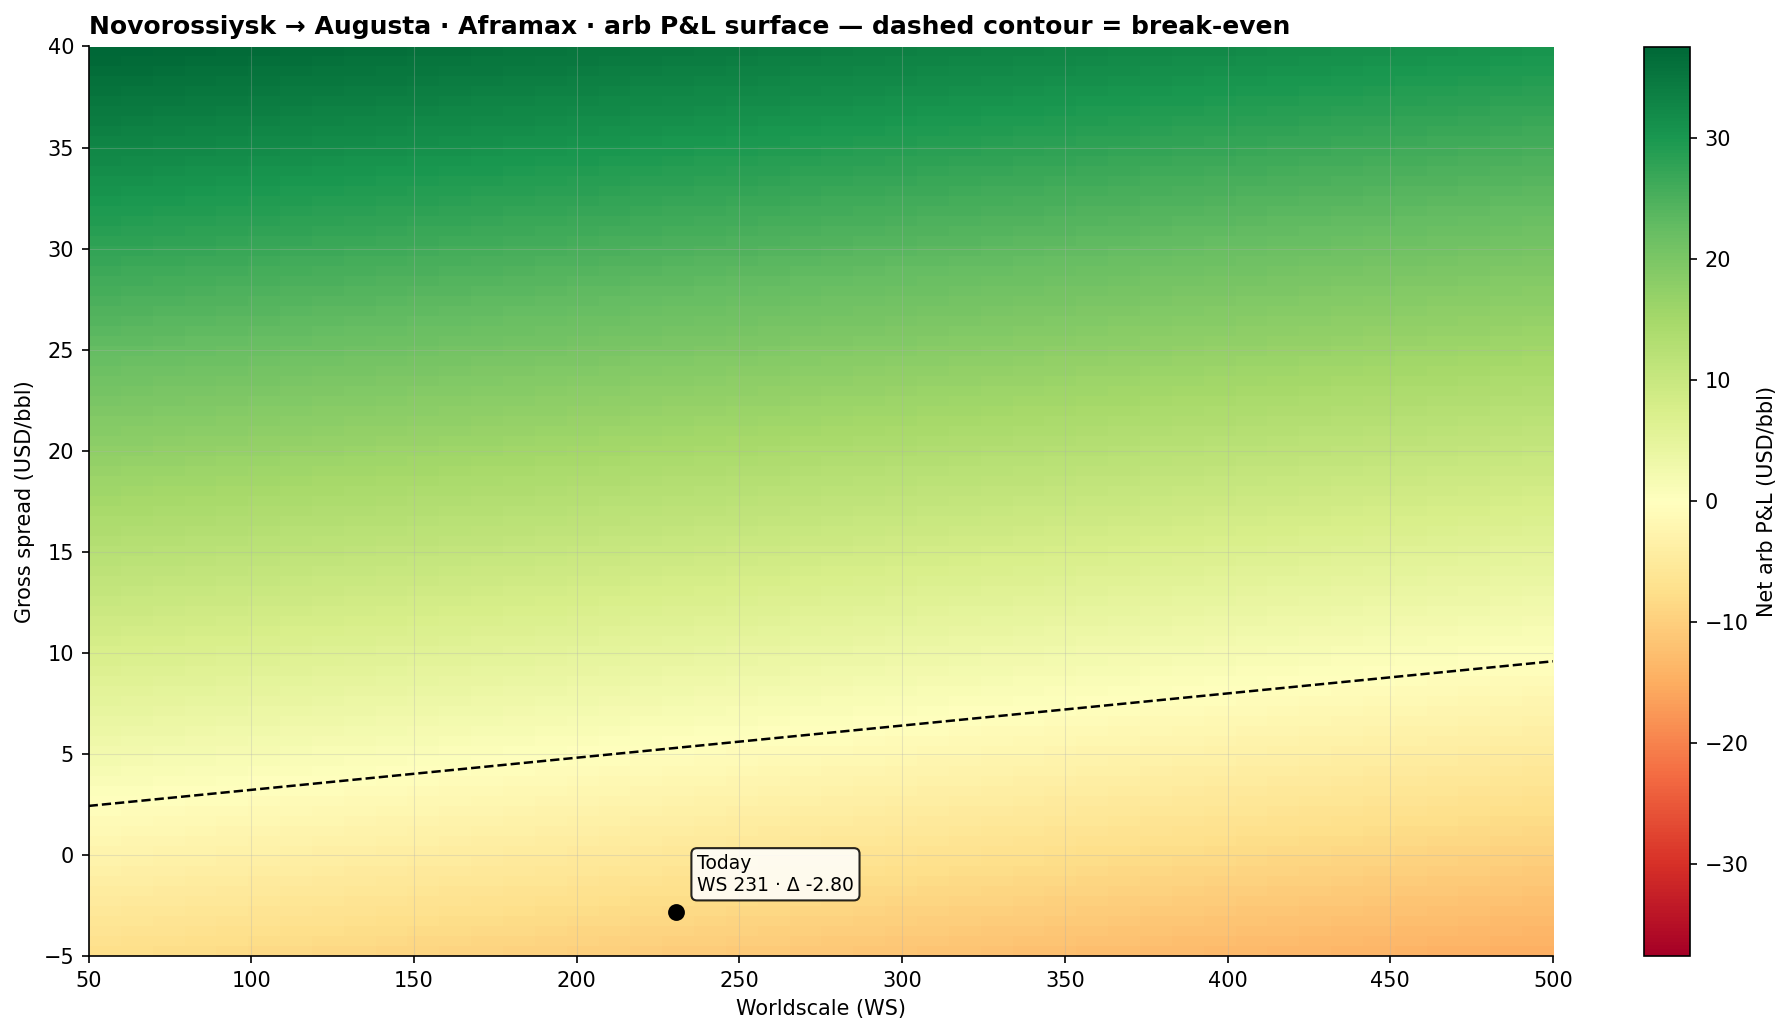
\includegraphics[width=\linewidth]{fig_11b_sensitivity_grid.png}\\[0.2cm]
{\footnotesize\textit{2-D P\&L surface on WS $\times$ gross spread (BSea $\rightarrow$ Med Aframax). Dashed contour is break-even; black dot marks the figure's snapshot operating point (WS 220, March/early-April regime, \emph{not} Apr 24). At Apr 24 the operating point would sit further right on the surface deep in negative-net territory.}}
\end{center}

\end{minipage}

\vspace{0.3cm}
\begin{callout}[Live Apr-24 waterfall, USG $\rightarrow$ \mbox{NWE} MR --- \emph{every line sourced}]
\footnotesize
\begin{tabular}{@{}lr@{\hspace{0.6em}}p{0.62\linewidth}@{}}
\textbf{Gross spread} & \textbf{+\$23.02/b} & \$173.49/b CIF \mbox{NWE} (AAVBG00, /7.45) $-$ \$150.47/b FOB USGC (AAXRV00, $\times$42) \\
Freight (WS$\times$flat) & $-$\$13.32/b & w405 $\times$ \$24.50/mt $\div$100 $\div$7.45 (MR Champion Arctic, BP, Apr 24) \\
Port costs           & $-$\$0.72/b   & USGC \$105k load + Rotterdam \$110k disch / 283k bbl \\
Canal tolls          & \$0.00         & no Suez/Panama on direct USG--ARA route \\
Financing            & $-$\$0.96/b   & SOFR 5.15\% + 300bps trader spread $\times$ \$170/b $\times$ 19/365 days \\
Insurance (P\&I+H\&M)& $-$\$0.45/b   & 25 bps of voyage value \\
\textbf{AWRP}        & \textbf{\$0.00} & USGC--NWE \emph{not} in war zone; AWRP is zero \emph{by route}, not by oversight. (BSea--Med lane: $-$\$0.80--\$1.50/b for context) \\
Demurrage            & $-$\$0.19/b   & 2 days $\times$ \$28k/day MR / 283k bbl \\
Broker commission    & $-$\$0.31/b   & 2.5\% of freight (industry standard) \\
\midrule
\textbf{Net arb}     & \textbf{+\$7.07/b}    & open arithmetically; physically constrained by ops/credit \\
\end{tabular}
\smallskip

\textbf{Reading.} On Apr 24 the gross USG--NWE ULSD spread (\$23/b) more than covers freight (\$13.3/b at w405) plus full cost stack. Net arithmetic: \textbf{+\$7/b}. The lane is therefore \emph{arithmetically open, operationally closed}: a BP-sized counterparty with FFA hedging can absorb the freight; a generic G7-linked desk paying spot freight at w405 with no FFA hedge and tighter vetting/credit gates cannot lift this margin. The waterfall is the upper bound; the trigger in \S\ref{sec:13} (sub-200 reopener) defines the \emph{executable} trade.

\smallskip
\textbf{Operational haircut --- quantified.} The +\$7.07/b clearing margin is not the executable margin. To turn arithmetic into execution, apply: (i) \textbf{30--50\% haircut} for vetting/credit/tonnage uncertainty $\rightarrow$ executable cushion needed of \$10--12/b before lifting; (ii) require \textbf{FFA hedge availability} on TC2 (currently illiquid above w400; sub-300 prints clear); (iii) require \textbf{confirmed MR tonnage} (Atlantic basin showing $<$10 prompt MR open, freight-finder data); (iv) min \textbf{\$50k absolute net} per cargo to clear desk-level minimum-size gates. Apr-24 \$7.07/b $\times$ 283 kbbl = \$2.0M absolute meets (iv), but fails (i)--(iii). \emph{Earlier editions ran the waterfall on a stale snapshot (WS 130, gross spread +\$7.39); the corrected Apr-24 numbers above replace that.}
\end{callout}

\vspace{0.2cm}
\begin{callout}[Break-even logic --- USG$\rightarrow$\mbox{NWE} MR, Apr 24]
\footnotesize
\textbf{Cost stack at Apr 24 inputs (everything except freight):} port \$0.72 + financing \$0.96 + insurance \$0.45 + AWRP \$0.00 + demurrage \$0.19 + broker \$0.31 = \textbf{\$2.63/b fixed.} \textbf{Freight elasticity:} freight per bbl = WS $\times$ \$24.50/mt $\div$ 100 $\div$ 7.45. WS 100 = \$3.29/b, WS 200 = \$6.58/b, WS 300 = \$9.87/b, WS 400 = \$13.16/b, WS 500 = \$16.44/b. \textbf{Break-even WS:} solve gross \$23.02/b $-$ \$2.63/b fixed $-$ freight = 0 $\rightarrow$ \$20.39/b freight cap $\rightarrow$ \textbf{WS $\approx$ 620.} \textbf{Net at WS sweep, Apr 24 gross:} w200 $\rightarrow$ +\$13.81/b, w300 $\rightarrow$ +\$10.52/b, w405 $\rightarrow$ \textbf{+\$7.07/b}, w500 $\rightarrow$ +\$3.95/b, w620 $\rightarrow$ \$0/b, w700 $\rightarrow$ $-$\$2.50/b. The \emph{executable} threshold is much tighter (sub-200 reopener in \S\ref{sec:13}) because it requires the gross to also rebuild post-de-escalation.
\end{callout}

\newpage

% ============================================================================
% SECTION 12 — ARB SCENARIOS
% ============================================================================
\section{Physical arbitrage: four historical scenarios}\label{sec:12}

\textit{The engine earns trust only if it reproduces what traders actually did under past conditions.}

\noindent\textcolor{obred}{\textbf{Desk decision.}} \emph{Each Crisis is regime-of-its-kind. 2022 was sanctions-gated (compliance binds), 2024-Red-Sea was freight-gated, 2026-Hormuz is operationally-gated. A desk model that treats them as one regime under-prices the binding gate.}

\vspace{0.2cm}

\begin{callout}[Hypotheses for every scenario]
\footnotesize
BSea $\rightarrow$ Med Aframax preset. Cargo: 80~kt Urals or alternate Russian-origin crude. Pricing: \emph{buy} at Novorossiysk = Brent M1 + premium/discount; \emph{sell} at Augusta = Brent M1 + Med basis. Voyage: $\sim$1{,}900 nm via Bosphorus, 6.6 days laden. Cost stack: SOFR+300bps financing, 25~bps insurance, broker 2.5\%, demurrage 2~days @\$40k. WS prints from Baltic / Howe Robinson; price prints from Platts \emph{Crude Oil Marketwire} of the date. \textbf{Spread shown below = realised commercial spread net of any prevailing Urals discount}, not paper Brent--Brent. AWRP for BSea--Med assumed +\$0.80--\$1.50/b throughout.
\end{callout}

\vspace{0.2cm}

\noindent\begin{minipage}[t]{0.48\linewidth}\vspace{0pt}

Four documented events plus the Apr-24 live regime, each replayed through the same calculator.

\vspace{0.15cm}
\textbf{2020-04 COVID} (WS 50, gross +\$3/b, engine net $\sim$+\$1/b). Real risk was flat-price volatility, not freight: paper Brent went briefly negative on the May-20 WTI roll, so a cargo carried \$20--30/b of intra-voyage P\&L variance.

\vspace{0.15cm}
\textbf{2022-03 Russia invasion} (WS 220, gross +\$35/b \emph{including} ${\sim}{-}\$30$ Urals discount). Widest print of the modern era; G7 price cap (Dec-2022) then closed Urals to compliant shipowners/insurers through 2023. \textbf{Cleanest demonstration of paper-basis vs executable-margin divergence under sanctions}.

\vspace{0.15cm}
\textbf{2024-01 Red Sea} (WS 145, gross +\$10/b, engine net negative once Cape routing adds 14--18 days). Nigerian crude flow to Asia dropped, rerouted West --- engine and market agree, closed.

\vspace{0.15cm}
\textbf{2026-04 Hormuz BSea$\rightarrow$Med} (WS 230, gross +\$28/b net of $-$\$15 Urals discount, engine net $\sim$+\$13/b). \emph{Compliance-gated} for G7 desks (Russian-origin crude, EU 20th package bans Tuapse) --- same pattern as 2022, reason the 2026 default lane is now USG$\rightarrow$\mbox{NWE} ULSD.

\vspace{0.15cm}
\textbf{2026-04 Apr-24 USG$\rightarrow$NWE ULSD} (WS 405, gross +\$23/b, engine net $\sim$+\$7/b clearing per \S\ref{sec:11}). \textbf{Live regime: \emph{arithmetically open, operationally closed}} for a generic G7 desk --- see trade idea \#3 in \S\ref{sec:13}.

\end{minipage}\hfill
\begin{minipage}[t]{0.50\linewidth}\vspace{0pt}

\begin{center}
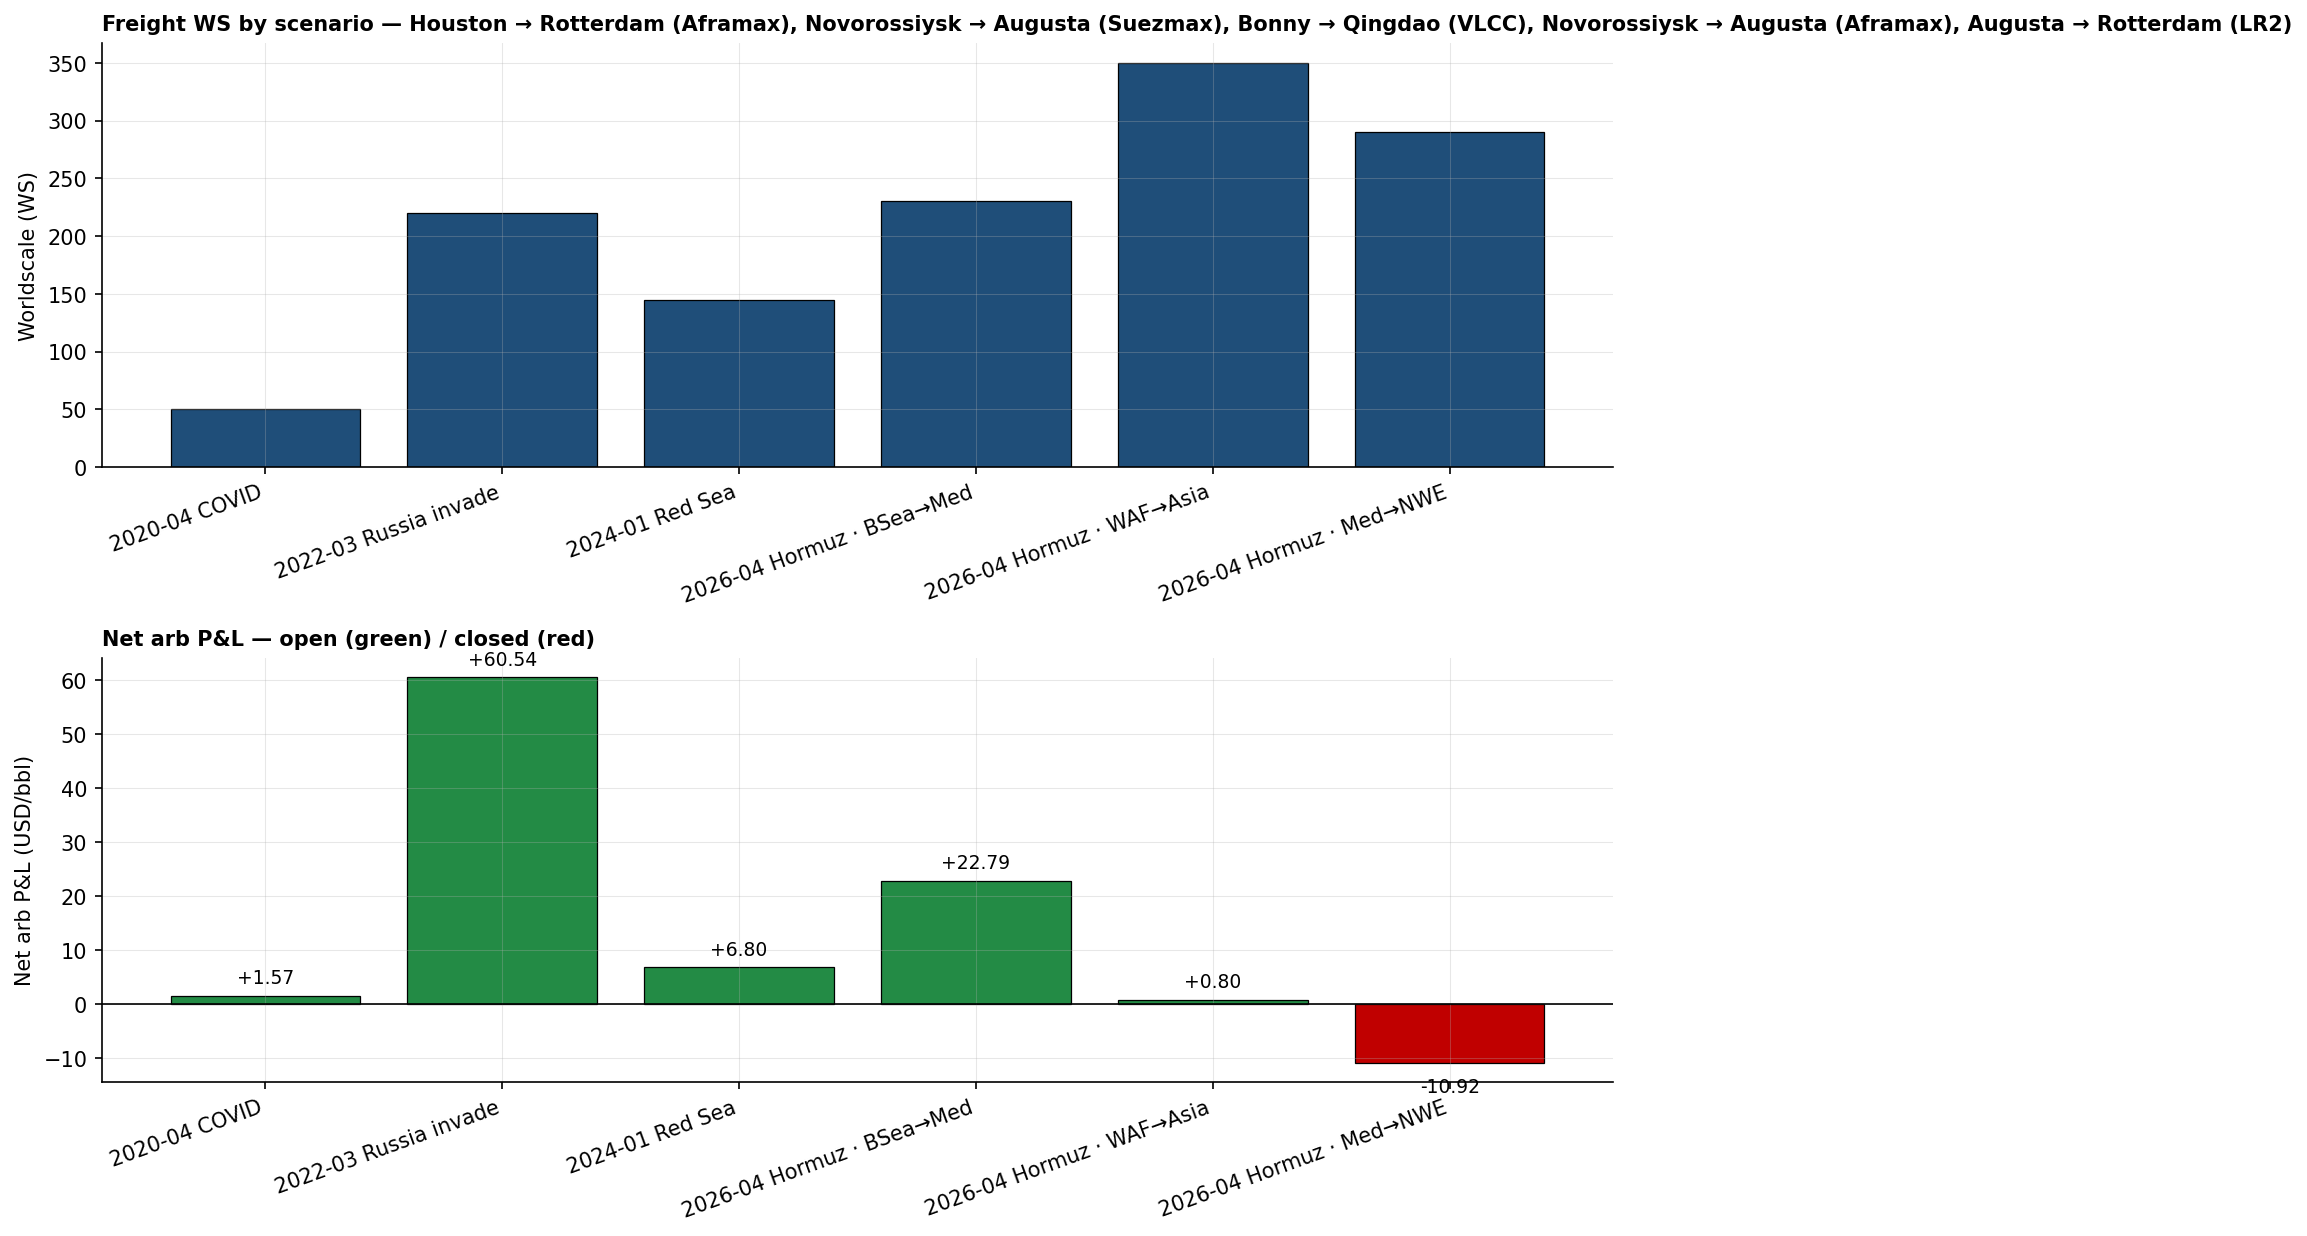
\includegraphics[width=\linewidth]{fig_12a_scenarios.png}\\[0.2cm]
{\footnotesize\textit{Scenario backtest, WS on top, net P\&L underneath.}}
\end{center}

\vspace{0.2cm}

\begin{center}
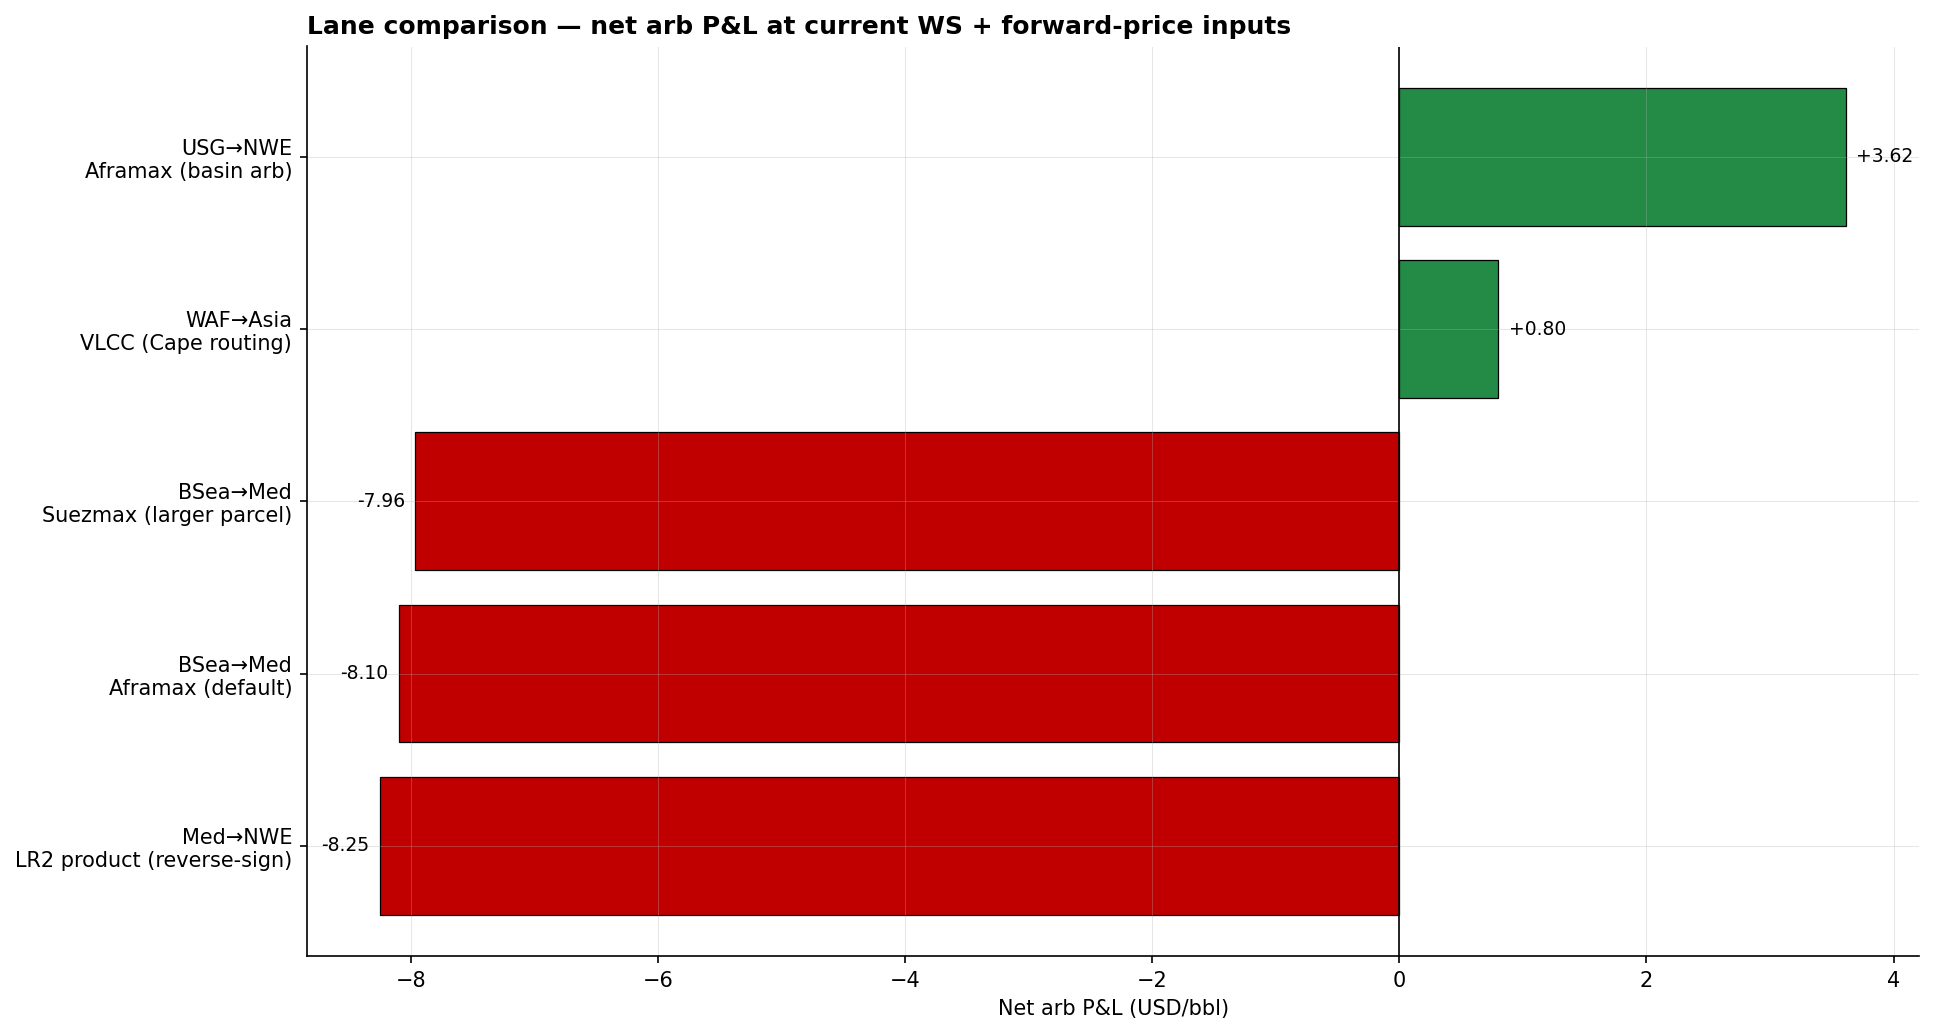
\includegraphics[width=\linewidth]{fig_12b_route_comparison.png}\\[0.2cm]
{\footnotesize\textit{Five canonical lanes, net P\&L at the WS / forward-price snapshot indicated per panel; not refreshed to Apr 24, see \S\ref{sec:11} for the live freight regime.}}
\end{center}

\end{minipage}

\vspace{0.25cm}
\begin{callout}[Logical cross-check vs public reporting]
\footnotesize
\begin{itemize}[leftmargin=1em,itemsep=0pt]
\item \textbf{2020-04 net $\sim$+\$1:} matches Vortexa / Kpler reporting that BSea cargoes lifted at near break-even economics, lane stayed open thinly.
\item \textbf{2022-03 net wide-open paper:} matches Reuters tape of Mar-Apr 2022 Urals discount blowout to $-$\$30, paper arb to $\sim$+\$30/b before sanctions architecture closed buyers.
\item \textbf{2024-01 closed:} matches the documented Nigeria-to-East flow rerouting and the BIMCO Cape-distance escalation.
\item \textbf{2026-04 BSea$\rightarrow$Med +\$13/b paper, compliance-gated:} consistent with EU 20th package timing (23-Apr) restricting Tuapse loadings.
\item \textbf{2026-04 USG$\rightarrow$NWE +\$7/b paper, operationally closed (not freight-closed):} matches the Apr-24 Champion Arctic w405 fixture and the Med--NWE inversion narrative in \S\ref{sec:1}.
\end{itemize}
\smallskip
\textbf{Which gate binds when.} Compliance is \emph{a} binding constraint, not the only one --- in 2022 and 2024 it was the binding gate; in 2024-01 (Red Sea) freight + voyage geometry dominated; in 2026-04 (USG$\rightarrow$NWE) operational/credit gates dominate (vetting, no FFA hedge, MR tonnage). A desk model that ignores any of these misses why the cargo didn't move at the printed price.
\end{callout}

\vspace{0.2cm}
%% [trailing bridge removed for pagination]

\newpage

% ============================================================================
% SECTION 13 — TRADING IDEAS
% ============================================================================
\section{Trading ideas, dated 24-Apr-2026}\label{sec:13}

\textit{Three observable, falsifiable trades that fall out of the evidence in the preceding pages.}

\noindent\textcolor{obred}{\textbf{Desk decision.}} \emph{Idea \#1 (Long ULSD crack, short Brent at $\beta=0.92$) is HIGH conviction --- enter today. Idea \#2 ULSD-EBOB pair is watchlist (mid-range). Idea \#3 USG$\rightarrow$NWE arb is watchlist on sub-200 freight reopener. Re-mark $\beta$ and trigger framework weekly.}

\vspace{0.2cm}

\noindent CIF Med ULSD prints \textbf{\$1,308.00/mt on Apr 24} (AAWYZ00, \emph{European Marketscan}), roughly 12\% over a normal-regime level and \$15.50/mt over CIF \mbox{NWE} (AAVBG00 \$1,292.50/mt). The Hormuz uncertainty is the main driver, and EU sanctions on Tuapse/Murmansk add a second compliance layer. The arb engine returns negative net on Med $\rightarrow$ \mbox{NWE}, the inverse of the structural trade, which is itself the signal that the clearing flow has flipped origin and destination for the week.

\vspace{0.2cm}

\begin{callout}[3-scenario forward framework, 30-day horizon]
\footnotesize
\setlength{\tabcolsep}{4pt}
\renewcommand{\arraystretch}{1.2}
\begin{tabular}{@{}p{0.16\textwidth}p{0.07\textwidth}p{0.13\textwidth}p{0.13\textwidth}p{0.13\textwidth}p{0.27\textwidth}@{}}
\toprule
\textbf{Scenario} & \textbf{Prob.} & \textbf{Brent (M1)} & \textbf{ULSD crack (matched)} & \textbf{MR Atl. WS} & \textbf{Trade implication} \\
\midrule
\textbf{De-escalation} (Tier-3) & 25\% & \$78--85/b ($-$\$20--27) & \$30--40/b ($-$\$28--38) & w150--220 ($-$200) & Kill Idea \#1 fast; Idea \#3 \emph{watchlist arms} sub-200; long EBOB cracker margin returns. \\
\textbf{Base} (current Tier-2 plateau) & 55\% & \$100--110/b (drift) & \$60--75/b (drift, mean +\$67) & w380--440 (range) & Hold Idea \#1 with stop; Idea \#2 fade if premium prints $>+$\$18/b; Idea \#3 closed. \\
\textbf{Escalation} (Tier-1, Strait closure) & 20\% & \$130--150/b ($+$\$25--45) & \$85--110/b ($+$\$15--40) & w500--700+ & Add Idea \#1 size, but fade aggressively into +\$100 crack; pivot to long Brent term-structure; close Idea \#3 hard. \\
\bottomrule
\end{tabular}
\smallskip

\textbf{Reading.} Probability weighting is anchored on Polymarket Hormuz contracts (live numbers below), OFAC-EU posture divergence (extension on US side, escalation on EU side $\rightarrow$ risk-balanced), and fixture activity (w405 prints today are inconsistent with imminent de-escalation). Each row's $\Delta$ Brent maps directly to the Tier-1/2/3 elasticities on p.~\pageref{sec:2}. Re-mark weekly against Hormuz transit data, CFTC positioning prints, and the Polymarket curve.
\end{callout}

\vspace{0.15cm}

\begin{callout}[Polymarket-implied Hormuz de-escalation curve --- pulled 2026-04-27]
\footnotesize
Market: \emph{``Strait of Hormuz traffic returns to normal by [date]''} (\path{polymarket.com/event/strait-of-hormuz-traffic-returns-to-normal-by-april-30}).
\smallskip

\begin{center}
\begin{tabular}{@{}lrr@{}}
\textbf{Resolution date} & \textbf{Cum. P(normal)} & \textbf{Marginal P, prior window} \\
\midrule
30-Apr-2026 & $<$1\%   & $<$1\% (Apr 27 $\rightarrow$ 30) \\
15-May-2026 & 21\%     & $\sim$20\% (May 1 $\rightarrow$ 15) \\
31-May-2026 & 38\%     & $\sim$17\% (May 16 $\rightarrow$ 31) \\
30-Jun-2026 & 60\%     & $\sim$22\% (June) \\
\end{tabular}
\end{center}

\smallskip
\textbf{Read.} The market prices a slow-grind de-escalation, not a sudden one --- roughly 20\% per 2-week window through end-June, near-uniform. \emph{(i)} The 25\% Tier-3 weighting in the table above is consistent with the May-15 timeline, not with end-June. \emph{(ii)} Idea \#1's 30-day exit is shorter than the market's de-escalation half-life --- 60-day exit or step-function take-profit fits the curve better. \emph{(iii)} The kill-switch geometry in \S\ref{sec:13} is real but not imminent: the next 4 weeks carry $\leq$21\% market-implied normalization, so position size on Idea \#1 can stay full through mid-May. There is also a separate live Polymarket market on \emph{``US x Iran permanent peace deal by [date]''} which moves slower than the Hormuz-traffic market and can be used as a confirmation signal --- watchlist, not an entry trigger.
\end{callout}

\vspace{0.2cm}

\subsection{Long \mbox{NWE} ULSD crack, short Brent hedge --- HIGH conviction}

\textbf{View.} Europe is structurally around 29 Mt/year short of diesel. US yields haven't moved on the distillate tilt despite the 2026 crack signal ($-17$ pp, unchanged). Hormuz keeps AG loadings depressed. Three asymmetries pointing the same way, with no yield response in sight. When that happens the clearing mechanism is price.

\textbf{Trade.} Long ULSD-only crack, not the 3-2-1 composite, because the signal is diesel-specific and the composite dilutes it. Hedge with Brent short, sized using the production-grade matched-calendar regime-conditional $\beta$ (see \S\ref{sec:5}): \textbf{Normal $\beta \approx 0$, Crisis-2026 mean $\beta = +0.61$, latest 30-day mean $+0.92$, latest single-day $+1.17$}. The trade sizes on the latest 30-day mean. A static pooled $\beta \approx 0.4$ would under-hedge by $\sim$50\% in this regime.

\textbf{Trigger.} ULSD crack above the in-sample 80th percentile \emph{and} US distillate stocks in the bottom quintile of the 5-year range. Both hit at 24-Apr-2026 close.

\textbf{Kill switch.} Credible Hormuz de-escalation headline. The 7 April ceasefire-rumour tape unwound jet cracks by 29 dollars in a single session, as a reference point for how fast this can reverse.

\begin{redbox}[Trade block --- Idea \#1]
\footnotesize
\begin{tabular}{@{}lp{0.74\linewidth}@{}}
\textbf{Signal}            & ULSD crack > IS 80th pct \emph{and} US distillate stocks in bottom quintile of 5y range. Both true at Apr-24 close. \\
\textbf{Trade}             & Long ULSD-NWE matched crack, short Brent hedge. 50{,}000 bbl ULSD-crack-equivalent. \\
\textbf{Entry}             & Apr-24 close: matched M2$\times$M1 crack \textbf{\$68.52/b} (vs naïve M1$\times$M1 \$62.32/b). \\
\textbf{Exit}              & Matched crack mean-revert below \$45/b, OR 30 calendar days, whichever first. \\
\textbf{Position size}     & For a 50{,}000-bbl ULSD-crack-equivalent: \textbf{67 LSGO swap lots} (1~lot = 100~mt $\approx$ 745~bbl $\rightarrow$ 67$\times$745 $\approx$ 49{,}900~bbl); \textbf{46 short Brent lots} (50{,}000 $\times$ 0.92 / 1{,}000 = 46, where $\beta=0.92$ is the production matched-M2$\times$M1 latest-30d mean, see \S\ref{sec:5}; 1 ICE Brent lot = 1{,}000~bbl). Recalibrate weekly: latest 60-d window mean is $0.66$ $\rightarrow$ 33 lots, latest single-day $\beta$ is $1.17$ $\rightarrow$ 58 lots. \\
\textbf{Expected P\&L}     & 1$\sigma$ crack mean-reversion $\approx$ \$8--10/b $\rightarrow$ \textbf{+\$400--500k}. \\
\textbf{Risk (downside)}   & Hormuz de-escalation compresses crack \$15--25/b in a session $\rightarrow$ \textbf{$-$\$750k to $-$\$1.25M}. \\
\textbf{Key driver}        & AG crude loading volume $\times$ EU diesel deficit (29 Mt/y). \\
\end{tabular}
\end{redbox}

\subsection{Fade the diesel-gasoline premium at extremes --- MED conviction}

\textbf{View.} The ULSD-EBOB crack premium is mean-reverting: anchored around +\$10/bbl, $\sigma$ around \$8, positive on more than 99\% of days because of Europe's structural diesel bias. Fade when it prints beyond +\$18 or below +\$2.

\textbf{Trade.} Short the premium at the +\$18 wide, long at +\$2.

\textbf{Trigger.} Today is mid-range, no signal. Watchlist weekly.

\textbf{Kill switch.} A structural regime change: EV adoption eroding diesel demand faster than expected, or a major hydrocracker closure shifting the output balance permanently.

\begin{redbox}[Trade block --- Idea \#2]
\setlength{\tabcolsep}{4pt}
\renewcommand{\arraystretch}{1.15}
\begin{tabular}{@{}p{0.21\textwidth}p{0.74\textwidth}@{}}
\textbf{Signal}            & ULSD-EBOB premium $>$+\$18/b (short) OR $<$+\$2/b (long). Anchored mean +\$10/b, IS-$\sigma$ \$8/b. \\
\textbf{Trade}             & Pair: short ULSD vs long EBOB at +\$18 wide; reverse at +\$2 narrow. NWE barrels both legs. \\
\textbf{Entry}             & Apr-24: not in zone (mid-range, no current trigger). \emph{Watchlist}. \\
\textbf{Exit}              & Mean-revert to +\$10 anchor OR 30 sessions, whichever first. \\
\textbf{Position size}     & 25{,}000 bbl/leg: \textbf{33 LSGO swap lots} ($\approx$24{,}600~bbl, 100~mt $\approx$ 745~bbl) and \textbf{30 EBOB swap lots} ($\approx$25{,}000~bbl, 100~mt $\approx$ 833~bbl gasoline density). \\
\textbf{Expected P\&L}     & 1$\sigma$ mean reversion $\approx$ \$8/b $\rightarrow$ \textbf{$+$\$200k} per trigger. \\
\textbf{Risk (downside)}   & Structural regime shift (EV demand drag, hydrocracker closure) before kill-switch fires $\rightarrow$ \textbf{$-$\$125k} convexity loss. \\
\textbf{Key driver}        & EU cracker output mix $\times$ diesel/gasoline import ratio (gasoline shoulder season + diesel structural deficit). \\
\end{tabular}
\end{redbox}

\subsection{USG $\rightarrow$ \mbox{NWE} ULSD arb --- MED/LOW conviction, watchlist}

\textbf{View.} This is the compliant default lane. The Med $\rightarrow$ \mbox{NWE} inversion closes the usual direction, so the relevant Atlantic trade for a G7-linked desk is USG $\rightarrow$ \mbox{NWE} ULSD on an MR tanker. \textbf{At Apr 24 fixture rate w405 (Champion Arctic, BP) the live waterfall in \S\ref{sec:11} clears \textbf{+\$7.07/b net} on a \$23.02/b gross USG--NWE spread.} The lane is therefore \emph{arithmetically open, operationally closed} for a generic G7 desk paying spot freight at w405 with no FFA hedge --- vetting / credit / tonnage gate the executable spread, not the math. This is a \emph{watchlist} trade conditional on Hormuz de-escalation reopening the executable margin, not a current-regime trade.

\textbf{Trade.} Long USG ULSD, short \mbox{NWE} ULSD, MR freight implied. Size with the Atlantic MR TCE and the \mbox{NWE} CIF level.

\textbf{Trigger.} \emph{Observable de-escalation signal first}: Hormuz transit count $>25$/day for 5 consecutive sessions (CAS daily). Then second-stage: MR Atlantic WS prints sub-200 \emph{and} CIF \mbox{NWE} ULSD holds above \$1,300/mt. Without the first signal, freight stays in the w400+ band and the arb stays closed.

\textbf{Kill switch.} A Hormuz de-escalation that reopens the usual Med $\rightarrow$ \mbox{NWE} trade and reverses the structural flow direction.

\begin{redbox}[Trade block --- Idea \#3]
\setlength{\tabcolsep}{4pt}
\renewcommand{\arraystretch}{1.15}
\begin{tabular}{@{}p{0.21\textwidth}p{0.74\textwidth}@{}}
\textbf{Signal}            & Hormuz transits $>$25/day for 5 consecutive sessions \emph{AND} MR Atlantic WS prints sub-200 \emph{AND} CIF \mbox{NWE} ULSD holds $>$\$1,300/mt. Two-stage trigger. \\
\textbf{Trade}             & Long USG FOB ULSD (AAXRV00), short \mbox{NWE} CIF ULSD (AAVBG00), MR freight implied. \\
\textbf{Entry}             & Apr-24: \emph{not} triggered. Live waterfall clears $+$\$7.07/b on a \$23.02/b gross spread; the binding constraint is \emph{operational} (vetting / credit / no-FFA / tonnage), \emph{not} freight. Watchlist only. \\
\textbf{Exit}              & Med $\rightarrow$ \mbox{NWE} usual flow reopens (Med lane reverses) OR Hormuz re-escalation collapses MR Atlantic freight back $>$w350. \\
\textbf{Position size}     & 1 MR cargo (38 kt $\approx$ 283 kbbl ULSD); 1 standard Atlantic MR voyage. \\
\textbf{Expected P\&L}     & Clearing margin \$7/b $\times$ 283 kbbl $\approx$ \textbf{$+$\$2.0M} gross of broker/financing on triggered cargo. \\
\textbf{Risk (downside)}   & Freight spike re-closes lane mid-voyage (WS jumps w200$\rightarrow$w400 in 48h, see Mar 2022) $\rightarrow$ \textbf{$-$\$1--2M} on the discharged cargo. \\
\textbf{Key driver}        & Hormuz transit rate (CAS daily) $\times$ MR Atlantic freight balance (Baltic / Argus). \\
\end{tabular}
\end{redbox}

\subsection{A note on sizing}

Everything above is illustrative. Real desk execution runs through vol-targeted Kelly, vehicle selection (swaps vs futures) for margin efficiency, broker commission, and firm-level risk limits. The part of these ideas that matters is the triggers: observable, falsifiable, unambiguous. The sizing numbers are placeholders until someone plugs them into a real P\&L book.

\vspace{0.2cm}
\textit{Methodology, data sources, and the explicit list of what the engine does \emph{not} model are on the closing pages.}

\newpage

% ============================================================================
% SECTION 14 — METHODOLOGY
% ============================================================================
\section{How it's built --- methodology, sources, caveats}\label{sec:14}

\subsection{The three engines}

\small
\begin{tabular}{@{}p{0.23\linewidth} p{0.72\linewidth}@{}}
\toprule
\textbf{\texttt{ForwardCurveAnalysis}} & ICE Brent / LSGO / WTI M1-M12 daily pre-rolled settlements. Term structure, volatility, IS-anchored Z-scores, CDF-calibrated regime classification, 2-state Gaussian HMM with BIC-based model selection. A cross-market module handles pair-wise correlation, rolling $\beta$, regime-conditional coupling, and basin spreads. \\
\addlinespace
\textbf{\texttt{CrackSpreadAnalysis}} & NWE / Med 3-2-1, 2-1-1, ULSD, EBOB, FO35 slates. Platts USD/MT to USD/bbl via density conversion. OPEC T76 as external cross-check. Gross refining margin (crack $\times$ throughput $\times$ utilisation, pre-opex) under normal-regime and war-crisis utilisation. Rolling $\beta$ can be conditioned on the \texttt{ForwardCurveAnalysis} LSGO regime flag for cross-engine hedging. HMM plus next-day forecast. \\
\addlinespace
\textbf{\texttt{CargoArb}} & Parametric 9-item P\&L waterfall. Origin, destination, vessel class, grade, cargo, WS, and flat rate all user-variable. Voyage days from distance / laden speed. Canal tolls, port costs, financing, insurance, demurrage, broker commission. Break-even solvable in WS or in spread. 2-D sensitivity grid with contour at zero P\&L. \\
\bottomrule
\end{tabular}

\subsection{Data sources}

\small
\begin{tabular}{@{}p{0.27\linewidth} p{0.42\linewidth} p{0.27\linewidth}@{}}
\toprule
\textbf{Domain} & \textbf{Source} & \textbf{As of} \\
\midrule
Forward curves        & Config \texttt{FORWARD\_PRICES\_USD\_BBL} & 2026-04-24 \\
Brent M1 / spot / Dated & ICE futures + Platts spot + Platts Dated & 2026-04-24 \\
Physical prints       & Platts European/AsiaPac/US Marketscan & 2026-04-24 \\
Tanker fixtures + WS  & Platts Dirty/Clean Tankerwire & 2026-04-24 \\
US stocks + util      & EIA weekly / monthly & 2026-04-17 \\
US yields             & EIA monthly & 2026-01 \\
EU stocks + consumption & Eurostat \texttt{nrg\_cb\_oilm} & 2026-02 \\
WS freight (annual)   & \emph{OPEC ASB 2025} T62 / T63 & 2011-2024 \\
Asia oil benchmarks   & SGX-DC final settlement (gasoil, VLSFO, naphtha) & 2026-04-22 \\
EU ETS allowance      & \texttt{prices\_eu\_ets\_all.csv} (weekly) & 2012-01 to 2026-04 \\
Sanctions --- US      & OFAC General License 134B (PDF) & 17-Apr-2026, exp.\ 16-May \\
Sanctions --- EU      & 20\textsuperscript{th} package, consilium.europa.eu & 23-Apr-2026 \\
\bottomrule
\end{tabular}

\subsection{What to keep in mind reading this}

A few things I'd want the reader to hold onto:

\begin{itemize}[leftmargin=1em,itemsep=0pt]
\item The out-of-sample window is 16 months. Any regime-frequency claim at that length has wide error bars. The direction is unambiguous, but the level --- "Crisis 31\%" for instance --- is descriptive of this episode, not a stable distribution estimate.
\item The Dated Brent file covers 69 days only, from 2 January to 14 April. Treated throughout as an event study, not a basis distribution.
\item The Z-score axis is capped at $\pm 5$ for readability. Actual peaks (LSGO around Z = 140) are annotated on-chart.
\item Eurostat publishes with a 2-3 month lag, so the most recent couple of months usually have only 1-2 reporting countries and get dropped from the aggregate charts.
\item The UK drops out of Eurostat after December 2020 (Brexit perimeter change, not a capacity collapse).
\item WS numbers in the \texttt{CargoArb} historical scenarios are triangulated from Baltic / Howe Robinson / Clarksons prints and public market reporting; per-scenario provenance lives in \path{Physical_Arb_Analysis/scenarios.yaml}.
\item This is not live. Every price is a dated snapshot. Cite 2026-04-24 when presenting the results.
\item \textbf{Data freshness varies by series.} Forward curves, physical prints, and tanker fixtures are 2026-04-24 (Platts Marketscan suite + ICE/NYMEX settles). US weekly stocks/util are 2026-04-17 (EIA). US monthly yields are 2026-01 (EIA). EU stocks and consumption are 2026-02 (Eurostat, 2--3 month lag). OPEC ASB freight is 2011--2024 (annual). Where a non-2026-04-24 series is cited in narrative the date is now stated inline.
\end{itemize}

\subsection{What the model does not do}

There are things I didn't build that a real desk would flag quickly. Bunker-price pass-through isn't modelled (WS flat rates assume a reference bunker). FFA forward-freight hedging isn't in the engine --- sensitivities assume spot WS throughout the voyage. Vetting gates (OCIMF SIRE, major-oil approvals) aren't modelled, which matters under sanctions. EU ETS maritime cost started phasing in during 2024 (40\% of emissions covered, rising to 70\% then 100\% through 2026) and isn't in the waterfall yet. The sanctions overlay goes as far as port flags; a proper jurisdictional compliance gate isn't there. Dirty-clean vessel switching option isn't priced. Laytime asymmetry between load and discharge ports is pooled. Counterparty, LC confirmation, and sovereign risk aren't modelled.

These are candidates for the next version, not flaws I'm trying to hide. The full list is in \path{Physical_Arb_Analysis/docs/BLIND_SPOTS_FULL.md}.

\subsection{Contract-month alignment (production-grade)}

A calendar helper (\texttt{Forward\_Curves\_Analysis/src/futures\_calendar.py}) handles contract-month matching between Brent and \mbox{LSGO}: because Brent rolls end of the second-month-preceding and \mbox{LSGO} rolls 2 business days before the 14th of the delivery month, the correct pairing flips twice per calendar month --- e.g. Brent M1 $\times$ \mbox{LSGO} M3 while \mbox{LSGO} has not rolled, Brent M1 $\times$ \mbox{LSGO} M2 after. The chartbook's matched-M2$\times$M1 crack uses the refiner-lag pairing (LSGO M1 product sold prompt vs Brent M2 crude bought one delivery month forward).

\textbf{Wiring complete.} The calendar pairing is now wired into production via \path{cross_market.py::matched_rolling_hedge_ratio(PAIRING='M2xM1')}, called from \path{scripts/run_matched_beta.py}. The regime-conditional $\beta$ printed in \S\ref{sec:5} is computed end-to-end from raw Excel strips $\rightarrow$ calendar pairing $\rightarrow$ rolling-OLS $\rightarrow$ regime aggregation. Output cached under \path{outputs/reports/matched_beta_by_regime.csv} (refresh date 2026-04-26). Full methodology in \path{CRACK_METHODOLOGY.md}.

\subsection{Three Brent series}

Brent M1 (ICE front-month futures settlement), Brent spot (Platts assessed close), and Dated Brent (Platts physical assessment at 16:30 London) are three different instruments. They diverge by dollars in calm tapes and by tens of dollars under stress; the April 2026 Dated-vs-M1 basis peaked at $\approx$\$35/bbl. The portfolio labels them distinctly everywhere they appear.

\subsection{Reproducibility}

Each project regenerates via \texttt{bash generate\_reports.sh} from its folder. Shared palette in \texttt{plot\_config.yaml}; event timeline in \texttt{major\_dates.yaml}. Chartbook source: \texttt{\_chartbook/Oil\_Portfolio\_Chartbook\_2026-04-24.tex} (LaTeX) plus \texttt{build\_pdf.py} (Python fallback).

\textbf{On refresh.} Charts update when source data is reloaded and notebooks re-executed; text commentary is dated to publication and does not auto-regenerate. Any dollar number the reader sees is as of 24-Apr-2026 close.

\newpage

% ============================================================================
% SECTION 15 — APPENDIX: HMM regime cross-check
% ============================================================================
\section{Appendix: HMM regime cross-check}\label{sec:15}

\textit{Full HMM detail. Body \S\ref{sec:3} keeps only the one-line cross-check.}

\vspace{0.2cm}

\begin{center}
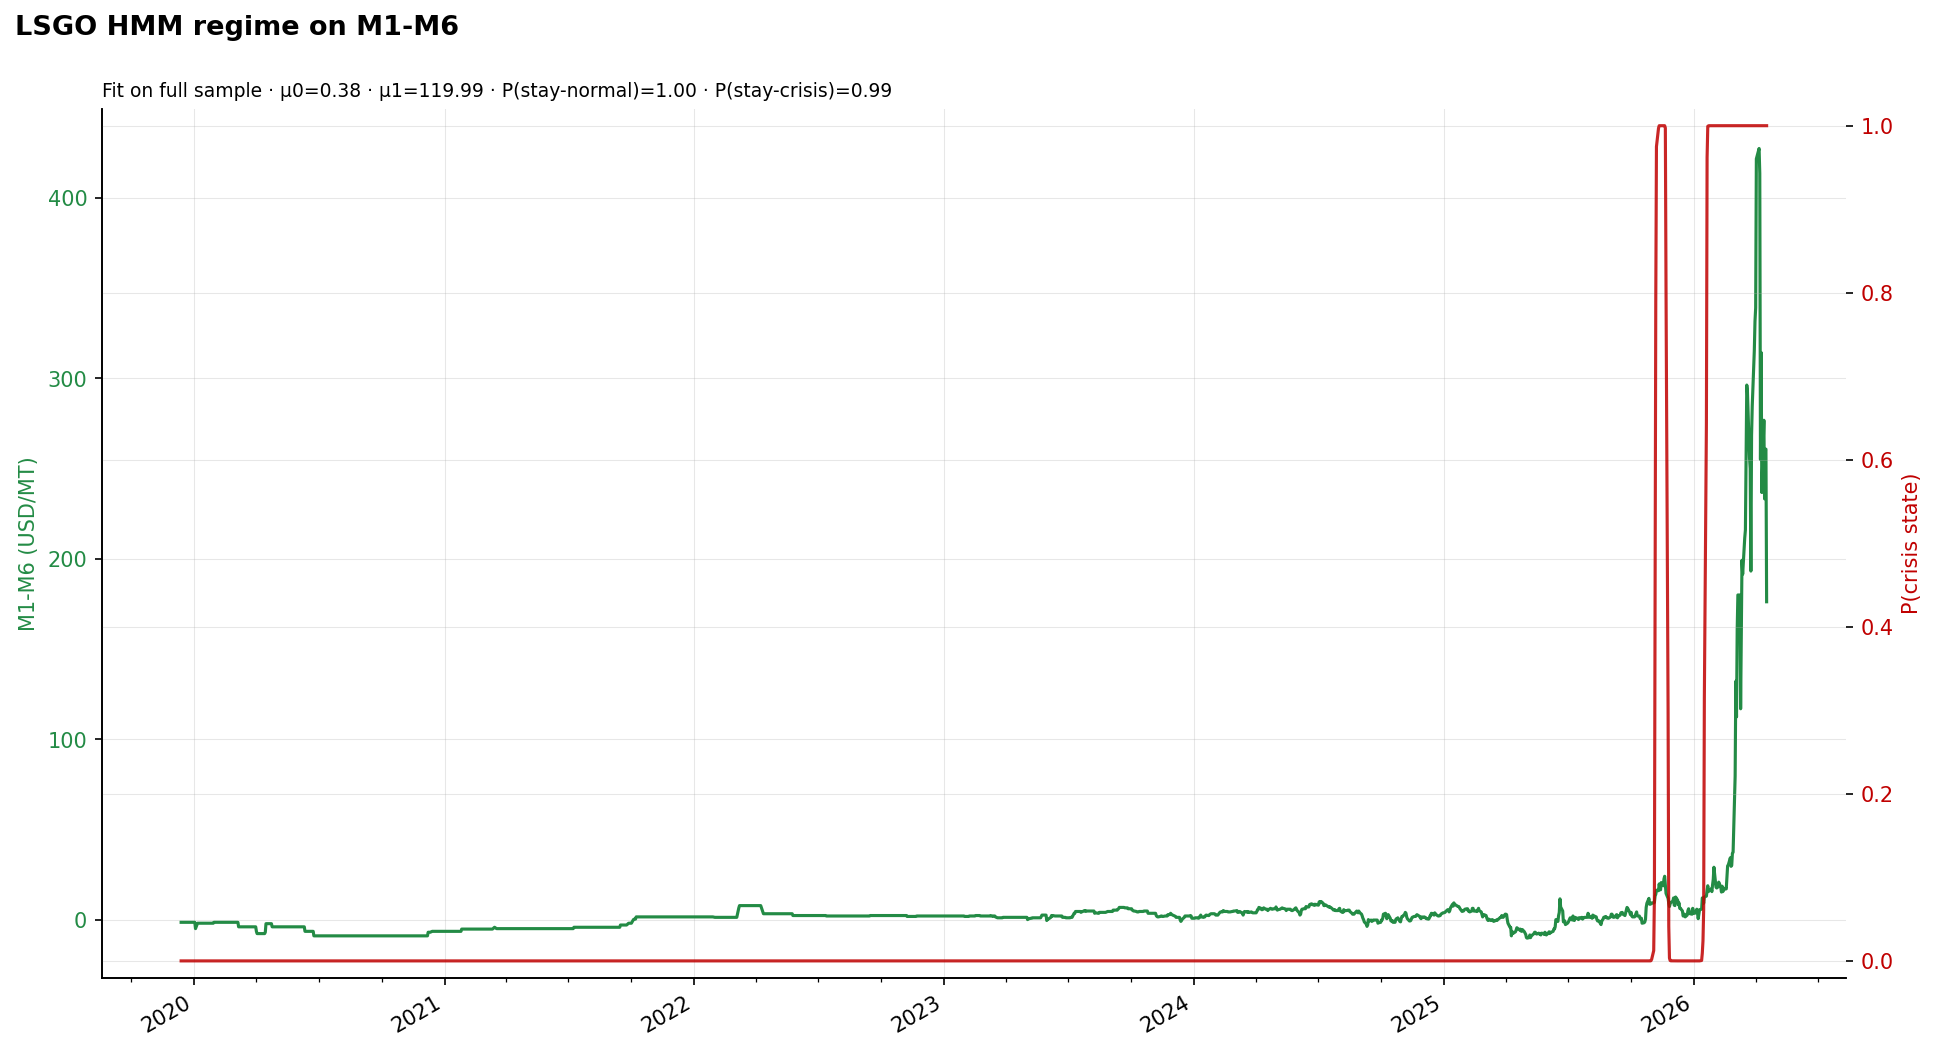
\includegraphics[width=0.78\linewidth]{fig_03c_lsgo_hmm.png}\\[0.2cm]
{\footnotesize\textit{Gaussian HMM on M1-M6. BIC prefers 2 states over 3 or 4 on this sample; next-day transition-matrix forecast in the underlying notebook.}}
\end{center}

\vspace{0.3cm}

\noindent\begin{minipage}[t]{0.48\linewidth}\vspace{0pt}
\begin{callout}[Why 2 states, not 3]
\footnotesize
The HMM output prints BIC for K$\in\{2,3,4\}$. K=2 minimises BIC by a comfortable margin. Adding states over-fits on the 16-month OOS, so the trade-off is between capturing more texture in the regime structure (3 states) and staying within what a small OOS can support (2 states). The 2-state fit agrees with the CDF classifier on the peak-Crisis window, which is the sanity check that matters.
\end{callout}
\end{minipage}\hfill
\begin{minipage}[t]{0.48\linewidth}\vspace{0pt}
\begin{callout}[What the HMM adds over the CDF]
\footnotesize
The CDF thresholds are level-based, so a regime flip fires when the spread crosses a fixed USD/MT line. The HMM reads the joint distribution of level, first difference and vol, so it picks up transitions before the level cut-off fires. In the 2026 data the HMM flagged the Crisis state about one week before the CDF threshold was breached.
\end{callout}
\end{minipage}

\vspace{0.3cm}
\textbf{Why this is appendix, not main body.} The HMM is a methodological sanity check. It does not generate an actionable early-warning trigger (1-week lead is shorter than the desk's typical position-adjustment cadence on a Crisis tape). The CDF classifier is the workhorse classifier in every cross-regime statistic in the body; the HMM merely confirms it.

\end{document}
